% -------------------------------
% Plantilla del TFM en la ESIIAB/ESICR de la UCLM. Version 0.1 (Preliminar)
%
% Compilar con XeLaTeX
% -------------------------------
\documentclass[12pt, a4paper]{book}

% -------------------------------
% Informacion y opciones del documento.
% -------------------------------
\input{include/opciones}

% -------------------------------
% Configuracion del documento, paquetes, etc.
% -------------------------------
\input{include/configuracion}

% Documento
\begin{document}

% -------------------------------
% Portada y titulo
% -------------------------------
\setmainfont[Ligatures={NoRequired,NoCommon,NoContextual}]{Calibri}
\input{elements/portada}

% -------------------------------
% Preambulo
% -------------------------------
\frontmatter
\input{elements/preambulo}

% -------------------------------
% Indices y tablas
% -------------------------------
\singlespacing

\tableofcontents
\listoffigures
\listoftables
\listofalgorithms
\listofcodes
\cleardoublepage

\onehalfspacing

% -------------------------------
% Documento principal
% -------------------------------
\mainmatter
\pagestyle{fancy}

\input{chapters/ch1}
\chapter{Estado del arte y marco tecnológico}

\section{Fundamentos y enfoques}

La movilidad urbana se ha consolidado como un ámbito de estudio en el que confluyen la ingeniería del transporte, la analítica de datos y la inteligencia artificial. En este contexto, los simuladores actuales no se limitan a representar mapas o a calcular rutas aisladas, sino que actúan como herramientas para evaluar políticas y escenarios de movilidad, permitiendo analizar de forma anticipada cómo cambios en los costes, en la oferta de transporte o en las condiciones operativas pueden modificar el comportamiento de la población.

Este tipo de sistemas exige combinar varias capas de conocimiento. Por un lado, la capa de datos, que determina la calidad y la trazabilidad de la información sobre la red de transporte y los servicios de transporte público asociados. Por otro, la capa de enrutado, que permite transformar un par origen-destino en variables de servicio observables (tiempo, distancia, segmentos de viaje, transbordos o coste aproximado). Finalmente, la capa de modelado, en la que dichas variables se integran con atributos sociodemográficos para estimar la elección modal y construir escenarios \textit{what-if}. Esta arquitectura en capas es coherente con la evolución reciente de herramientas de simulación en investigación y planificación \cite{Horni2016MATSim,Lopez2018SUMO}.

%%%%%%%%%%%%% PARA INTRODUCCIÓN CH1 %%%%%%%%%%%%%%%%%%
% \begin{figure}[h]
%     \centering
%     \includegraphics[width=\textwidth]{figs/ch2_pipeline2.png}
%     \caption{Esquema conceptual del flujo de información en un simulador de movilidad como el desarrollado en este TFM. Elaboración propia.}
%     \label{fig:ch2_pipeline}
% \end{figure}

\section{Datos abiertos para movilidad}

El desarrollo de los sistemas descritos en el apartado anterior requiere la disponibilidad de grandes volúmenes de datos fiables y reutilizables. Por este motivo, en los últimos años han adquirido gran protagonismo los conjuntos de datos abiertos en movilidad, ya que permiten construir, validar y reproducir modelos de análisis sin depender de fuentes propietarias cerradas. En este contexto, OpenStreetMap y GTFS se han consolidado como los dos pilares más utilizados para representar, respectivamente, la red urbana y la oferta de transporte público.

\subsection{OpenStreetMap}

OpenStreetMap (OSM) es una base de datos geográfica abierta y colaborativa ampliamente utilizada en proyectos de movilidad, tanto en investigación como en aplicaciones operativas. La propia fundación del proyecto define OSM como una fuente de datos abiertos reutilizable por terceros, con cobertura global y actualización continua por parte de la comunidad \cite{OSMAbout}. Esta naturaleza abierta resulta especialmente relevante en un trabajo experimental, ya que permite reproducir resultados a partir de un conjunto de datos público, versionable e independiente de condiciones comerciales impuestas por terceros.

En términos de calidad cartográfica, diversos estudios han mostrado que OSM puede ofrecer niveles de precisión adecuados para el análisis del transporte, aunque con cierta heterogeneidad espacial entre zonas y entre tipos de elemento, por ejemplo, entre la red viaria principal y los detalles de la infraestructura peatonal \cite{Haklay2010}. Por ello, en este trabajo OSM se considera una fuente adecuada para construir la red de enrutado, teniendo en cuenta las características específicas del área de estudio al interpretar los resultados.

\subsection{GTFS}

GTFS (\textit{General Transit Feed Specification}) es el estándar abierto dominante para publicar oferta de transporte público programada. La documentación oficial describe de forma precisa el contrato de datos entre productor y consumidor: estructura de ficheros, relaciones entre entidades y restricciones semánticas necesarias para que un planificador pueda reconstruir correctamente servicios, horarios y calendarios \cite{GTFSReference}. En otras palabras, GTFS no es solo un formato de intercambio, sino también un marco común de interoperabilidad entre operadores, agregadores y motores de planificación.

La estructura del estándar se basa en un conjunto de ficheros fundamentales, entre los que destacan \texttt{stops.txt}, \texttt{routes.txt}, \texttt{trips.txt}, \texttt{stop\_times.txt}, \texttt{calendar.txt} y \texttt{calendar\_dates.txt}. Estos archivos permiten representar simultáneamente la topología de la red y la dimensión temporal del servicio \cite{GTFSReference}. Esta separación resulta esencial, ya que el componente espacial define dónde se presta el servicio y el componente temporal determina cuándo se presta. En un entorno de simulación multimodal, ambos planos deben mantenerse coherentes para evitar itinerarios inviables o resultados inconsistentes.

En el contexto español, el canal institucional más relevante para localizar y descargar feeds GTFS es el \textit{Punto de Acceso Nacional de Transporte Multimodal} (NAP), gestionado por el Ministerio de Transportes y Movilidad Sostenible. La propia descripción oficial del portal lo define como el punto único nacional para concentrar información de oferta de transporte de viajeros, en línea con el marco europeo de datos de movilidad \cite{NAPHome,NAPQuienesSomos}.

En este TFM, la descarga de datos para transporte urbano se realizó precisamente desde NAP. Como ejemplo de referencia nacional se consultó el conjunto de EMT Valencia y, para el caso de estudio del proyecto, el conjunto de autobuses urbanos de Toledo \cite{NAPEMTValencia,NAPToledoUrbano}. En ambos casos, la página de detalle expone metadatos operativos (por ejemplo, número de paradas y formatos de descarga), así como los atributos incluidos en el conjunto de datos, como la accesibilidad, las tarifas o la geometría de las rutas. Esta información permite verificar de forma rápida el tamaño y la estructura del feed antes de integrarlo en el flujo de procesamiento del simulador.

La propia comunidad GTFS publica recomendaciones de calidad de publicación (persistencia de identificadores, estabilidad de URL de feed, cobertura temporal mínima y buenas prácticas de consistencia), que son relevantes para garantizar explotación automatizada en entornos de producción o experimentación \cite{GTFSBestPractices}. Además, el validador canónico mantenido por MobilityData se ha convertido en herramienta estándar para control de calidad de feeds estáticos antes de su uso analítico \cite{GTFSValidator}. En este trabajo, GTFS cumple una doble función: por un lado, alimentar la capa de consulta de la red de autobús urbano y, por otro, proporcionar los datos necesarios para construir el grafo multimodal empleado posteriormente por OpenTripPlanner.

\section{Tecnologías abiertas de enrutado}

Una vez descritas las fuentes de datos que permiten representar la red urbana y la oferta de transporte público, la segunda pieza fundamental de un simulador de movilidad es el algoritmo de enrutado. Estos motores permiten transformar la información geoespacial y temporal en itinerarios concretos, así como obtener variables de servicio relevantes, como el tiempo de viaje, la distancia recorrida, los transbordos o las fases de acceso y egreso. En este trabajo se emplean dos tecnologías abiertas con funciones complementarias: OSRM, orientado al cálculo eficiente de rutas sobre red viaria, y OpenTripPlanner, especializado en planificación multimodal con transporte público.

\subsection{OSRM}

OSRM (\textit{Open Source Routing Machine}) es uno de los motores abiertos más utilizados para cálculo de rutas sobre red viaria OSM, especialmente cuando se necesitan tiempos de respuesta bajos y gran volumen de consultas \cite{OSRMDocs,OSRMGitHub}. Su interés en un simulador de movilidad no está solo en obtener una ruta entre dos puntos, sino en poder generar de forma sistemática atributos de viaje (tiempo, distancia o matrices origen-destino) que después se integran en análisis y modelos predictivos.

La principal fortaleza técnica de OSRM es su enfoque de preprocesado: antes de servir consultas, el sistema transforma el extracto \texttt{.osm.pbf}, que es el formato binario comprimido habitualmente utilizado para distribuir datos de OpenStreetMap, en estructuras optimizadas de búsqueda. Este diseño desplaza coste al inicio, pero permite consultas rápidas y estables durante la fase de explotación. Además, OSRM trabaja con perfiles de movilidad diferenciados (por ejemplo, coche, bicicleta y a pie), lo que permite modelar de forma explícita costes de viaje distintos por modo. A nivel interno, OSRM se apoya en algoritmos de aceleración de rutas: MLD (\textit{Multi-Level Dijkstra}), que divide la red en niveles para reducir el espacio de búsqueda en cada consulta, y CH (\textit{Contraction Hierarchies}), que simplifica el grafo con atajos para acelerar rutas largas~\cite{Delling2017CRP,Geisberger2008CH}.
% En este trabajo se prioriza MLD por su equilibrio entre rendimiento y flexibilidad, dejando CH como alternativa

% En este TFM, lo más importante no es solo la velocidad, sino el control local del proceso. Ejecutar OSRM en infraestructura propia permite fijar exactamente qué versión de software, qué versión de red y qué perfiles se usan en cada experimento. Eso evita cambios externos no controlados y hace que los resultados sean comparables entre iteraciones. En un flujo con muchas simulaciones e inferencias, este control local mejora la trazabilidad y la reproducibilidad de forma directa.

\subsection{OpenTripPlanner}

OpenTripPlanner (OTP) es un planificador multimodal diseñado para combinar red de calle (OSM) y red de transporte público programado (GTFS) en un único problema de viaje puerta a puerta \cite{OTPDocs,OTPGitHub}. Su función difiere de la de un motor de enrutado viario convencional, ya que no se limita a calcular el tramo sobre la red de calles, sino que también representa de manera integrada las fases de acceso peatonal, los tiempos de espera, el recorrido en transporte público, los posibles transbordos y el tramo final hasta el destino.

La documentación oficial de OTP describe una arquitectura basada en construcción previa de grafo y posterior explotación por API de planificación. Ese grafo integra simultáneamente geometría de red y programación temporal del servicio, por lo que la consulta de rutas depende de fecha y hora, no solo de coordenadas \cite{OTPBuildConfig,OTPRouteRequest}. Esta dimensión temporal es la base para representar transporte público de forma operativa.

En la salida, OTP devuelve itinerarios descompuestos en tramos o segmentos de viaje, denominados \textit{legs} en su propia documentación, con información sobre el modo utilizado, los tiempos parciales, el número de transbordos y los metadatos de cada línea. Esta estructura resulta especialmente útil para el análisis multimodal, ya que permite distinguir con precisión las distintas fases del desplazamiento. Por contraste, motores viarios como OSRM están orientados al cálculo rápido de rutas sobre red de calle y no incorporan de forma nativa la lógica propia del transporte público, con horarios, transbordos y secuencias diferenciadas dentro de un mismo itinerario.


\section{Plataformas propietarias y servicios gestionados}

Junto a las tecnologías abiertas de enrutado, el ecosistema actual de movilidad incluye también plataformas propietarias que ofrecen estos mismos servicios mediante API gestionadas. La relevancia industrial de este problema ha favorecido la aparición de soluciones comerciales muy maduras, orientadas tanto al desarrollo de producto como a la integración rápida en aplicaciones web y móviles. Aunque estas plataformas simplifican el despliegue técnico, también introducen condicionantes específicos en términos de coste, dependencia del proveedor y reproducibilidad.

\subsection{Google Maps Platform}

Google Maps Platform se ha convertido en un estándar de facto en los servicios comerciales de localización y navegación orientados al desarrollo de productos digitales. En particular, \textit{Routes API} ofrece cálculo de rutas multimodo, metadatos de viaje y un ecosistema de integración especialmente maduro para aplicaciones web, móviles y, de forma destacada, entornos basados en Android \cite{GoogleRoutesAPI}.

Para proyectos de desarrollo de producto, este modelo reduce de forma notable la complejidad operativa, ya que no exige desplegar ni mantener infraestructura propia de enrutado y permite acceder a funcionalidades avanzadas mediante API. Esta característica ha favorecido su adopción en aplicaciones comerciales, especialmente en entornos móviles y ecosistemas integrados con servicios de Google. No obstante, en contextos de investigación aplicada o en escenarios con un volumen elevado de simulaciones, aparecen limitaciones relevantes: por un lado, el coste económico crece con el número de peticiones y con el tipo de servicio consumido; por otro, la ejecución queda condicionada por cuotas de uso, políticas del proveedor y disponibilidad externa de la plataforma \cite{GoogleMapsPricing}. Estas restricciones reducen su idoneidad cuando se busca trazabilidad completa, control experimental y escalabilidad económica predecible.

\subsection{Otras plataformas de referencia}

Además de Google Maps Platform, el ecosistema actual incluye otras alternativas consolidadas de consumo por API, entre ellas Mapbox \cite{MapboxDirectionsAPI} o TomTom \cite{TomTomRoutingAPI}. Estas plataformas ofrecen catálogos amplios (rutas, matrices, navegación, tráfico y servicios avanzados según proveedor), y comparten una lógica común de uso gestionado mediante credenciales, límites de consumo y planes de servicio.

También existen servicios intermedios como openrouteservice, que proporcionan API pública y, al mismo tiempo, opciones de despliegue propio \cite{OpenRouteServiceAPI,OpenRouteServiceRestrictions}. Este tipo de solución puede ser útil como puente entre experimentación rápida y control de infraestructura, aunque con sus propias restricciones de uso en modalidad pública.

La Tabla~\ref{tab:routing_comparison} resume esta comparación y la decisión tecnológica adoptada en el proyecto. Para un simulador académico orientado a experimentación, trazabilidad y ejecución repetida de escenarios, la combinación OSRM + OTP en infraestructura propia ofrece un equilibrio más adecuado que una API comercial gestionada, aunque implique una mayor complejidad de despliegue.

\begin{table}[ht]
    \centering
    \caption{Comparación resumida de las soluciones de enrutado consideradas en este trabajo. Elaboración propia a partir de \cite{OSRMDocs,OTPDocs,GoogleRoutesAPI,GoogleMapsPricing}.}
    \label{tab:routing_comparison}
    \begin{tabular}{L{2.0cm}L{2.8cm}L{2.8cm}L{4.0cm}}
        \hline
        \textbf{Solución} & \textbf{Tipo de red} & \textbf{Coste de uso} & \textbf{Adecuación al TFM} \\
        \hline
        OSRM & Red viaria OSM, perfiles por modo & Infraestructura propia & Muy adecuado para consultas masivas y control experimental \\
        \hline
        OTP & Red multimodal OSM + GTFS & Infraestructura propia & Muy adecuado para transporte público y análisis puerta a puerta \\
        \hline
        Google Maps Platform & API comercial multimodo gestionada & Pago por petición y cuotas & Útil como referencia industrial, menos adecuado para reproducibilidad \\
        \hline
    \end{tabular}
\end{table}

\section{Modelado de elección modal}

Una vez descrita la infraestructura tecnológica que permite representar la red y calcular itinerarios, es necesario incorporar una capa de modelado que permita analizar el comportamiento de los viajeros. En un simulador de movilidad, no basta con conocer qué alternativas existen para un desplazamiento determinado, sino que también es necesario estimar cuál de ellas es más probable que sea elegida en función de sus atributos de servicio y de las características del usuario. Esta cuestión se aborda habitualmente mediante modelos de elección discreta y, más recientemente, mediante técnicas de aprendizaje automático aplicadas a la predicción de la elección modal \cite{Train2009,MartinBaos2023Thesis}.

En la literatura reciente, una de las referencias más utilizadas para este tipo de problemas es el dataset London Passenger Mode Choice (LPMC), construido a partir de viajes observados en Londres y enriquecido con variables de nivel de servicio para distintos modos de transporte \cite{Hillel2018LPMC,CSLPMC2019}. Su interés en este trabajo no está en el caso de estudio concreto, sino en que proporciona una base metodológica y experimental muy próxima al problema abordado en este TFM.

\subsection{Modelos de utilidad aleatoria}

Este problema se ha abordado tradicionalmente mediante los denominados modelos de utilidad aleatoria (\textit{Random Utility Models}, RUM), ampliamente utilizados en transporte para analizar decisiones de elección discreta, como la elección del modo de transporte. En este enfoque, el decisor elige una alternativa dentro de un conjunto de opciones mutuamente excluyentes, por ejemplo caminar, usar la bicicleta, utilizar transporte público o desplazarse en coche \cite{Train2009,McFadden1974}.

La idea central de estos modelos es que cada viajero asocia una utilidad a cada alternativa disponible dentro de su conjunto de elección, y se asume que elegirá aquella que le proporcione una mayor utilidad. Sin embargo, dicha utilidad no puede observarse de forma completa, ya que parte de los factores que influyen en la decisión sí pueden ser medidos por el analista, mientras que otros permanecen ocultos o no observados. Por ello, la utilidad de una alternativa suele descomponerse en un término determinista y un término aleatorio:
\begin{equation}
U_{in} = V_{in} + \varepsilon_{in}
\end{equation}
donde $U_{in}$ representa la utilidad total que el individuo $n$ asocia a la alternativa $i$, $V_{in}$ es la componente sistemática o determinista de dicha utilidad, y $\varepsilon_{in}$ recoge los factores no observados que también influyen en la decisión.

Bajo este planteamiento, el viajero se considera racional en el sentido de que selecciona la alternativa que maximiza su utilidad. En consecuencia, la elección observada puede expresarse en términos probabilísticos como la probabilidad de que la utilidad de una alternativa sea mayor o igual que la del resto de alternativas disponibles:
\begin{equation}
P_{in} = P(U_{in} \geq U_{jn}\ \forall j \in C)
\end{equation}
donde $C$ representa el conjunto de alternativas consideradas. De este modo, los RUM permiten traducir un problema de comportamiento individual en un modelo probabilístico de elección, capaz de relacionar atributos del viaje, características del individuo y probabilidad de seleccionar cada modo de transporte.

\subsection{Modelo Logit Multinomial}

Entre los modelos derivados del enfoque RUM, el más extendido en el análisis de elección modal es el Modelo Logit Multinomial (\textit{Multinomial Logit}, MNL). Su popularidad se debe a que ofrece una formulación matemática sencilla, una interpretación clara de los parámetros y una estimación relativamente eficiente desde el punto de vista computacional. En el contexto del transporte, el MNL ha sido utilizado de forma recurrente para estudiar cómo variables como el tiempo de viaje, el coste, los transbordos o determinadas características sociodemográficas influyen en la probabilidad de elegir un modo de transporte frente a otro \cite{McFadden1974}.

El modelo MNL se obtiene al asumir que el término aleatorio de la utilidad sigue una distribución Gumbel independiente e idénticamente distribuida para todas las alternativas. Bajo esta hipótesis, la probabilidad de que el individuo $n$ elija la alternativa $i$ puede expresarse de la siguiente forma:
\begin{equation}
P_{in} = \frac{\exp(V_{in})}{\sum_{j=1}^{I}\exp(V_{jn})}
\end{equation}
donde $I$ es el número total de alternativas disponibles y $V_{in}$ representa la utilidad sistemática de la alternativa $i$ para el individuo $n$. Esta expresión da lugar a una función de probabilidad de tipo sigmoidal, de manera que pequeñas variaciones en la utilidad representativa tienen mayor efecto cuando la probabilidad de elección se encuentra en valores intermedios que cuando una alternativa ya es claramente dominante o claramente poco atractiva. Esta propiedad resulta especialmente útil para interpretar cambios marginales en los atributos del servicio, por ejemplo ante mejoras en tiempo o coste de una determinada alternativa.

La Figura~\ref{fig:mnl_sigmoid} ilustra de forma esquemática esta forma sigmoidal de la probabilidad de elección en el modelo MNL.


\begin{figure}[ht]
    \centering
    \includegraphics[width=0.6\textwidth]{figs/mnl_sigmoid.png}
    \caption{Forma sigmoidal ilustrativa de la probabilidad de elección en el modelo MNL. Elaboración propia.}
    \label{fig:mnl_sigmoid}
\end{figure}

En la práctica, la componente determinista de la utilidad suele especificarse como una combinación lineal de atributos observables:
\begin{equation}
V_{in} = \beta_{i0} + \sum_{k}\beta_{ik}x_{ink}
\end{equation}
donde $x_{ink}$ representa el valor del atributo $k$ asociado a la alternativa $i$ para el individuo $n$, $\beta_{ik}$ es el parámetro que mide la influencia de dicho atributo y $\beta_{i0}$ es una constante específica de la alternativa. Esta formulación permite cuantificar el efecto relativo de variables como el tiempo de viaje, el coste monetario, el número de transbordos o el acceso peatonal, entre otras. En términos interpretativos, los parámetros estimados indican cómo varía la utilidad de cada modo cuando cambian sus atributos observables.

La estimación de los parámetros del modelo se realiza habitualmente mediante máxima verosimilitud. Para ello, se define una función de verosimilitud que mide la probabilidad de observar las elecciones registradas en la muestra dadas unas determinadas estimaciones de los parámetros. El objetivo del proceso de ajuste consiste en encontrar los valores de $\beta$ que maximizan dicha verosimilitud, o de forma equivalente, que maximizan la log-verosimilitud del modelo. Este procedimiento constituye la base clásica de estimación de modelos de elección discreta y permite obtener un modelo interpretable y coherente con la teoría del comportamiento del viajero.

En este TFM, el modelo MNL resulta relevante como referencia metodológica, ya que proporciona una base teórica sólida para representar la elección modal a partir de atributos del desplazamiento. Además, sirve como punto de comparación frente a enfoques más flexibles basados en aprendizaje automático, que se describen en los apartados siguientes.

Una limitación conocida del modelo MNL es la hipótesis de independencia de alternativas irrelevantes (\textit{Independence of Irrelevant Alternatives}, IIA), derivada de la suposición de errores independientes e idénticamente distribuidos. Esta propiedad implica que la relación de sustitución entre dos alternativas no depende de la presencia o de las características del resto de modos, lo cual puede resultar restrictivo en problemas de movilidad donde algunas opciones están más correlacionadas entre sí que otras \cite{McFadden1974,Train2009}. Aun así, el MNL sigue siendo el punto de partida más habitual en la literatura por su equilibrio entre simplicidad, interpretabilidad y capacidad descriptiva.



\subsection{Limitaciones del enfoque clásico}

A pesar de su amplia utilización en el análisis de elección modal, los modelos basados en utilidad aleatoria presentan ciertas limitaciones cuando se aplican a problemas complejos de movilidad. En primer lugar, requieren especificar de forma explícita la forma funcional de la utilidad sistemática, lo que implica que el analista debe decidir previamente qué variables incluir y cómo se relacionan con la utilidad de cada alternativa. En muchos casos, esta especificación se realiza mediante combinaciones lineales de atributos del viaje, lo que puede resultar restrictivo cuando las relaciones reales entre variables son no lineales o presentan interacciones complejas \cite[p.~20]{MartinBaos2023Thesis}.

Otra limitación relevante es que los modelos clásicos suelen asumir estructuras relativamente simples en la distribución de los términos de error. En el caso del modelo Logit Multinomial, por ejemplo, la hipótesis de independencia de alternativas irrelevantes puede no reflejar adecuadamente situaciones en las que algunas alternativas presentan correlaciones más fuertes entre sí, como ocurre frecuentemente entre distintos modos de transporte público o entre modos motorizados.

Además, desde un punto de vista práctico, la especificación de modelos econométricos puede requerir un proceso iterativo de selección de variables, transformación de atributos y validación de supuestos teóricos. Aunque este enfoque proporciona modelos interpretables y coherentes con la teoría del comportamiento del viajero, puede resultar menos flexible cuando se trabaja con conjuntos de datos de alta dimensionalidad o con relaciones complejas entre variables.


\subsection{Aprendizaje automático para elección modal}

Con el aumento de la disponibilidad de datos y de la capacidad computacional, en los últimos años han ganado relevancia los enfoques basados en aprendizaje automático para el análisis de elección modal. Desde esta perspectiva, la elección de modo puede formularse también como un problema de clasificación supervisada, en el que el objetivo consiste en predecir la alternativa elegida a partir de un conjunto de variables explicativas relacionadas con el viaje y con las características del individuo.

A diferencia de los modelos clásicos de elección discreta, muchos algoritmos de aprendizaje automático no requieren especificar de forma explícita la forma funcional de la relación entre variables. En su lugar, aprenden patrones directamente a partir de los datos de entrenamiento, lo que les permite capturar relaciones no lineales, interacciones complejas entre atributos y estructuras de decisión difíciles de representar mediante modelos lineales tradicionales.

Entre las técnicas más utilizadas en este contexto destacan los métodos basados en árboles de decisión y los modelos de conjunto (\textit{ensemble models}) derivados de ellos, como Random Forest o Gradient Boosting Decision Trees, así como los modelos basados en redes neuronales profundas. Estos enfoques han mostrado un rendimiento predictivo competitivo en numerosos problemas de clasificación tabular, incluyendo aplicaciones en transporte y elección modal.

En este trabajo se adopta esta perspectiva complementaria: el modelo Logit Multinomial se considera como referencia metodológica clásica, mientras que distintos modelos de aprendizaje automático se utilizan para explorar alternativas con mayor capacidad predictiva. En particular, la arquitectura del simulador se ha diseñado para permitir la integración de diferentes modelos de clasificación, entre ellos Random Forest, Gradient Boosting Decision Trees y redes neuronales profundas, de forma que puedan compararse sus resultados en el contexto del problema de elección modal analizado. Esta comparación resulta coherente con la evidencia reciente disponible para datasets reales de elección modal, entre ellos LPMC \cite{Hillel2018LPMC}.

\subsection{Random Forests}

Random Forest es un método de aprendizaje automático basado en la combinación de múltiples árboles de decisión entrenados sobre subconjuntos distintos de los datos. El modelo fue propuesto por Breiman \cite{Breiman2001} como una extensión de los árboles de clasificación tradicionales, con el objetivo de mejorar su estabilidad y capacidad predictiva. En diversas revisiones de la literatura, este tipo de modelos aparece además como una de las familias más utilizadas en comparativas recientes de elección modal.

La idea fundamental consiste en entrenar un gran número de árboles de decisión sobre diferentes subconjuntos de los datos de entrenamiento. Cada árbol se construye utilizando una muestra aleatoria del conjunto de datos original (técnica conocida como \textit{bootstrap sampling}) y, además, en cada división del árbol se considera únicamente un subconjunto aleatorio de variables explicativas. Este doble proceso de aleatorización permite reducir la correlación entre árboles individuales y, en consecuencia, mejorar el rendimiento del modelo agregado.

En problemas de clasificación, como el de elección modal, cada árbol produce una predicción independiente y la decisión final se obtiene mediante votación mayoritaria entre todos los árboles del bosque. Este mecanismo permite capturar relaciones no lineales entre variables y manejar de forma robusta conjuntos de datos con múltiples atributos.

En el ámbito del transporte, los modelos Random Forest se han utilizado en distintos trabajos para predecir la elección de modo de transporte, ya que ofrecen un buen equilibrio entre capacidad predictiva, robustez frente al sobreajuste y relativa facilidad de interpretación mediante medidas de importancia de variables. No obstante, la evidencia comparativa reciente sugiere que su rendimiento puede quedar por debajo del de otros métodos más potentes de boosting en algunos conjuntos de datos reales \cite{MartinBaos2023TRC}.

\subsection{Gradient Boosting Decision Trees}

Los modelos basados en \textit{Gradient Boosting Decision Trees} (GBDT) constituyen otra familia de métodos de aprendizaje automático ampliamente utilizados en problemas de clasificación con datos tabulares. A diferencia de los métodos basados en bagging, como Random Forest, el enfoque de boosting construye los árboles de decisión de forma secuencial, de modo que cada nuevo árbol intenta corregir los errores cometidos por el conjunto de árboles anteriores \cite{Friedman2001}.

El proceso comienza entrenando un primer árbol de decisión sencillo sobre los datos de entrenamiento. A continuación, se construyen árboles adicionales que se ajustan sobre los residuos o errores del modelo previo. De este modo, el modelo final se obtiene como la suma ponderada de múltiples árboles débiles, cada uno de los cuales contribuye a mejorar gradualmente la predicción global.

Entre las implementaciones más conocidas de este enfoque se encuentra XGBoost (\textit{Extreme Gradient Boosting}), una biblioteca optimizada que introduce mejoras en eficiencia computacional, regularización del modelo y manejo de grandes conjuntos de datos \cite{Chen2016XGBoost}. Gracias a estas características, XGBoost se ha convertido en una de las técnicas más utilizadas en problemas de aprendizaje supervisado con datos estructurados y ha mostrado un comportamiento especialmente competitivo en comparativas recientes de elección modal.

En el contexto de este TFM, los modelos basados en Gradient Boosting resultan especialmente relevantes, ya que permiten capturar relaciones no lineales entre los atributos del viaje y la elección modal. Además, su buen rendimiento predictivo y su flexibilidad para manejar distintos tipos de variables los convierten en una herramienta adecuada para integrarse en el simulador de movilidad desarrollado en este trabajo.

\subsection{Redes Neuronales Profundas}

Las redes neuronales profundas (\textit{Deep Neural Networks}, DNN) constituyen otra familia de modelos de aprendizaje automático que ha experimentado un crecimiento significativo en los últimos años. Estas técnicas se basan en arquitecturas formadas por múltiples capas de neuronas artificiales que transforman progresivamente las variables de entrada mediante combinaciones lineales y funciones de activación no lineales \cite{Goodfellow2016}.

A diferencia de los modelos basados en árboles, las redes neuronales permiten aprender representaciones internas de los datos a través de varias capas ocultas, lo que facilita capturar relaciones complejas entre variables. Esta capacidad de modelar interacciones no lineales ha motivado su aplicación en numerosos problemas de predicción y clasificación, incluyendo el análisis del comportamiento de los viajeros.

En problemas de elección modal, las redes neuronales profundas pueden utilizarse para estimar la probabilidad de seleccionar cada modo de transporte a partir de atributos del desplazamiento y características sociodemográficas del usuario. Aunque estos modelos suelen requerir mayor volumen de datos y un proceso de ajuste más cuidadoso que los métodos basados en árboles, también ofrecen una elevada flexibilidad para capturar patrones complejos presentes en los datos.

Los tres enfoques descritos en esta sección (Random Forest, Gradient Boosting y redes neuronales profundas) se evalúan de forma comparativa sobre el dataset LPMC. Su entrenamiento, ajuste e integración en el simulador de movilidad se detallan en el capítulo~\ref{ch:implementacion}.

% En este trabajo, las redes neuronales profundas se consideran como una posible extensión del sistema de predicción implementado en el simulador de movilidad. La arquitectura del sistema permite integrar distintos modelos de clasificación, lo que abre la posibilidad de incorporar en futuras versiones modelos neuronales entrenados sobre los mismos atributos de viaje utilizados por los métodos basados en árboles.

%%%%%%%%%%%%%%%%%%%%%%%%%%%%%%%%%%%%%%%%%%%%%%%%%%%%%%%%%%%%%

% REVISAR COMENTARIO (3 o 4 carillas)

% Puedes sacar cosas para este apartado de mi tesis doctoral (capítulo 2): https://ruidera.uclm.es/bitstreams/e13f06da-2cbd-4ca1-a026-99a53401b348/download

% Índice propuesto:

% Primero motivas que una vez se dispone de la infraestructura que modela la red, es necesario analizar el comportamiento de los pasajeros.

% - Modelos de utilidad aleatoria

% Random Utility Models (RUM) en inglés. Se han usado desde los años 70 para analizar el comportamiento de los viajeros en redes de transporte. Son modelos clásicos. Asumen que los decisores (los viajeros) son racionales y eligen la alternativa (de transporte) que maximiza su utilidad. 

% Cuenta un poco como va (páginas 14 y 15 de mi tesis)


% - Modelo Logit Multinomial

% Multinomial Logit (MNL) model. Cuentas un pcoo como funciona de forma sencillita y como se usa en este caso para modelar la elección de modo. Pon alguna figura como la Figura 2.1 de mi tesis. También fórmulas como la (2.3) que es sencilla y necesaria, o la (2.4). Nada super complejo. Que te ocupe en general 1 o 2 caras. Di que se ajustan mediante la minimización de una función de pérdida, en este caso se máximiza la verosimilitud del modelo. Poco más. No entres en detalles super técnicos.


% - Modelos de Aprendizaje Automático

% Los modelos RUM tienen limitaciones (en mi tesis vienen detalladas, tu solo comentalas sin entrar en detalle). Por eso se proponen modelos de Aprendizaje Automático.... (2 párrafos o así).


% Subapartados: (1 subapartado cortito por cada modelo que usemos en el TFM)

% -- Random Forests

% -- Gradient Boosting Decision Trees

% -- Redes Neuronales Profundas


% \missingfigure




% \subsection{Modelos clásicos y ML tabular}

% La modelización clásica de elección modal se fundamenta en la teoría de utilidad aleatoria y en modelos de elección discreta como MNL, ampliamente consolidados en transporte \cite{Train2009,McFadden1974}. Estos modelos destacan por interpretabilidad y base teórica, pero pueden quedar limitados cuando aparecen no linealidades complejas o interacciones de alta dimensión.

% En paralelo, modelos de ML tabular como Random Forest y XGBoost han mostrado un rendimiento predictivo competitivo en numerosos problemas de clasificación \cite{Breiman2001,ChenGuestrin2016}. En elección modal, su principal fortaleza es la capacidad de capturar patrones no lineales con poca ingeniería manual de variables.

% \subsubsection{Fortalezas y debilidades}

% \textbf{Modelos clásicos (MNL y derivados)}:
% \begin{itemize}
%   \item fortaleza: interpretabilidad económica y consistencia conductual;
%   \item debilidad: menor flexibilidad ante estructuras complejas.
% \end{itemize}

% \textbf{ML tabular (RF y XGBoost)}:
% \begin{itemize}
%   \item fortaleza: alta capacidad predictiva desagregada;
%   \item debilidad: mayor dificultad para interpretación comportamental directa.
% \end{itemize}

% Estudios recientes comparativos en datasets reales de elección modal muestran precisamente este compromiso entre precisión, interpretabilidad y coste computacional \cite{MartinBaos2023TRC}.

% \subsection{Modelos neuronales}

% Las redes neuronales profundas (DNN) constituyen una alternativa para capturar relaciones complejas entre atributos de viaje y características del individuo. Su uso en elección modal ha crecido en la literatura reciente, especialmente en contextos con alta dimensionalidad.

% \subsubsection{DNN y consideraciones prácticas}

% En la práctica, su rendimiento depende de decisiones de arquitectura (profundidad y anchura), regularización y validación. Entre las técnicas habituales, dropout sigue siendo estándar para reducir sobreajuste durante entrenamiento \cite{Srivastava2014Dropout}. En implementaciones con Keras/TensorFlow, dropout se aplica en entrenamiento y se desactiva automáticamente en inferencia \cite{TensorflowDropout}.

% Para este TFM, la línea DNN se plantea como vía paralela de investigación comparativa respecto al modelo base XGBoost, priorizando ejecución en CPU para simplificar reproducibilidad en entorno local.
% \section{Dataset LPMC}

% \subsection{Características del dataset}

% El dataset LPMC (London Passenger Mode Choice) recoge información detallada de desplazamientos y variables sociodemográficas relevantes para modelar elección modal. Su descripción y material suplementario de recreación de choice-sets han sido publicados en el caso de estudio de Londres \cite{Hillel2018LPMC}.

% En el ecosistema del proyecto, LPMC se utiliza como base para entrenar y evaluar el modelo de clasificación modal (\texttt{walk}, \texttt{cycle}, \texttt{pt}, \texttt{drive}), manteniendo separación temporal train/test y pipeline reproducible.


% El uso de LPMC en un simulador aplicado a Toledo implica una transferencia de conocimiento entre contextos urbanos diferentes. Esto aporta valor como prueba de concepto, pero obliga a explicitar límites de validez externa en la interpretación de resultados.

% Como referencia metodológica de comparación de modelos y criterios de evaluación (desagregados y agregados), este trabajo se apoya además en la evidencia reciente publicada por Martín-Baos et al. \cite{MartinBaos2023TRC}, que analiza de forma sistemática modelos clásicos y de aprendizaje automático en elección modal.

% \missingfigure

\chapter{Metodología}
\label{ch:metodologia}

Este capítulo recoge la gestión del proyecto con un enfoque SCRUM adaptado a un TFM individual. Se busca dejar trazabilidad clara de qué se planificó, qué se ejecutó, qué bloqueos aparecieron y qué decisiones técnicas se tomaron en cada iteración.


\section{SCRUM adaptado a un desarrollo unipersonal}

SCRUM es una metodología ágil de carácter iterativo e incremental, orientada a organizar el trabajo en ciclos cortos, priorizar entregas de valor y revisar de forma continua el avance del producto \cite{ScrumGuide2020}. Aunque su formulación original está pensada para equipos, sus principios también pueden adaptarse a proyectos individuales cuando se busca mantener planificación, trazabilidad y capacidad de reacción ante cambios.

En este trabajo se ha utilizado una adaptación práctica de SCRUM, no como aplicación estricta del marco en todos sus elementos formales, sino como guía para estructurar el desarrollo del simulador, registrar decisiones y ordenar la evolución del proyecto. Esta adaptación ha resultado útil por tres motivos. En primer lugar, porque se han combinado tareas heterogéneas, incluyendo desarrollo backend, frontend, integración de motores de enrutado, tratamiento de datos, entrenamiento de modelos y redacción de memoria. En segundo lugar, porque el alcance real del proyecto ha ido evolucionando a medida que se validaban soluciones técnicas y se detectaban bloqueos. Por último, porque el seguimiento periódico con el tutor ha funcionado como mecanismo natural de revisión y reorientación.

Desde el punto de vista organizativo, la Guía Scrum 2020 define un \textit{Scrum Team} compuesto por tres responsabilidades principales: \textit{Product Owner}, \textit{Scrum Master} y \textit{Developers} \cite{ScrumGuide2020}. En un trabajo unipersonal esta separación no puede reproducirse de forma literal, por lo que se ha reinterpretado del siguiente modo:
\begin{itemize}
  \item \textbf{Product Owner}: el tutor académico ha asumido de forma aproximada esta función, al validar prioridades, orientar el alcance funcional del prototipo y revisar la utilidad de los entregables desde el punto de vista del objetivo del TFM.
  \item \textbf{Scrum Master}: esta responsabilidad ha sido asumida por el propio autor del trabajo, en la medida en que ha organizado iteraciones, registrado bloqueos, mantenido la trazabilidad del progreso y ajustado la planificación cuando han surgido incidencias técnicas o cambios de enfoque.
  \item \textbf{Developers}: el desarrollo técnico también ha recaído íntegramente en el autor, responsable de la implementación del simulador, la integración de servicios, el entrenamiento de modelos y la documentación de resultados.
\end{itemize}

En consecuencia, varias responsabilidades propias de un equipo Scrum han quedado concentradas en una única persona, mientras que el tutor ha actuado como agente externo de supervisión, validación y priorización. Esta circunstancia introduce diferencias claras respecto a un SCRUM de equipo, pero no invalida su uso como marco ligero de gestión. En este contexto, lo más relevante no ha sido reproducir todas las ceremonias de forma estricta, sino conservar los elementos que aportan valor real al proyecto: backlog priorizado, trabajo por iteraciones, revisión periódica y registro explícito de decisiones.

La metodología seguida en este trabajo se ha apoyado en los siguientes principios:
\begin{itemize}
  \item dividir el trabajo en sprints con objetivos acotados y entregables identificables;
  \item mantener un \textit{Product Backlog} vivo, revisado conforme avanzaba el proyecto;
  \item registrar en cada iteración qué se planificó, qué se completó y qué problemas aparecieron;
  \item utilizar las reuniones con el tutor como mecanismo de revisión y re-priorización;
  \item orientar cada sprint a la obtención de un incremento funcional o documental del proyecto.
\end{itemize}

En cuanto al seguimiento, las reuniones con el tutor comenzaron a finales de 2025, aproximadamente entre octubre y noviembre, con una periodicidad quincenal, normalmente los martes. Una vez finalizado el primer cuatrimestre y superada la carga principal de exámenes, la cadencia pasó a ser semanal a partir de febrero y marzo de 2026, con el objetivo de acelerar el ritmo de desarrollo y acotar con mayor precisión el trabajo asociado a cada sprint. Este cambio de frecuencia reforzó el carácter iterativo del proyecto y facilitó una validación más cercana del backlog y de los entregables.

La Figura~\ref{fig:scrum_tfm_cycle} resume visualmente este ciclo de trabajo adaptado a un desarrollo unipersonal, mostrando la relación entre backlog, planificación, ejecución y revisión periódica con el tutor.

\begin{figure}[ht]
    \centering
    \includegraphics[width=0.78\textwidth]{figs/scrum_tfm_cycle.png}
    \caption{Esquema del ciclo de trabajo SCRUM adaptado al desarrollo unipersonal del proyecto. Elaboración propia.}
    \label{fig:scrum_tfm_cycle}
\end{figure}

Esta metodología ha encajado bien con la naturaleza del proyecto. Por una parte, ha permitido avanzar de manera incremental desde un prototipo inicial de rutas hasta un MVP funcional con integración de OSRM, OTP, GTFS y un modelo de elección modal. Por otra, ha facilitado documentar de forma ordenada tanto el trabajo ya completado como las líneas de evolución previstas, incluyendo mejoras visuales, ampliación de modelos y posibles análisis adicionales de simulación. A partir de este marco general, en los apartados siguientes se presenta el backlog del proyecto y el histórico de sprints ejecutados.

\section{Product Backlog}

\subsection{Backlog inicial}

El \textit{Product Backlog} se definió como una lista viva de trabajo, organizada en grandes bloques funcionales y técnicos. En lugar de partir de un conjunto cerrado de tareas detalladas desde el inicio, se optó por un backlog de alto nivel que pudiera refinarse a medida que se validaban decisiones de diseño y se consolidaba el MVP del simulador.

En una primera aproximación, los elementos principales del backlog fueron los siguientes:

\begin{enumerate}
  \item Definir una arquitectura base cliente-servidor para desacoplar frontend, backend y servicios externos.
  \item Construir un prototipo web funcional con mapa interactivo, selección de origen-destino y visualización de rutas.
  \item Integrar OSRM en local con perfiles diferenciados para coche, bicicleta y desplazamiento a pie.
  \item Incorporar transporte público urbano mediante GTFS de Toledo y OpenTripPlanner.
  \item Diseñar una API propia que unifique consultas de rutas, exploración GTFS e inferencia modal.
  \item Preparar una pipeline reproducible de datos para el dataset LPMC.
  \item Entrenar y validar un primer modelo de elección modal utilizable dentro del simulador.
  \item Integrar el modelo de inferencia en backend y frontend de forma modular.
  \item Mejorar la interfaz, la experiencia de usuario y la capacidad de análisis visual del sistema.
  \item Documentar la solución, registrar la evolución del proyecto y redactar la memoria final.
\end{enumerate}

Conforme avanzó el trabajo, este backlog se fue refinando en tareas más concretas. Algunos elementos inicialmente planteados como trabajo futuro pasaron a formar parte del desarrollo principal, mientras que otros quedaron aplazados para iteraciones posteriores. A fecha de redacción de esta memoria, la parte nuclear del simulador puede considerarse ya implementada, por lo que el backlog actual se concentra principalmente en consolidación documental, mejoras visuales y ampliaciones funcionales sobre una base ya operativa.

Para facilitar su seguimiento, los elementos del backlog se agruparon en cuatro bloques:
\begin{itemize}
  \item \textbf{Bloque funcional}: interfaz web, selección de viajes, cálculo de rutas, visualización de resultados y cuadro de información.
  \item \textbf{Bloque de integración de servicios}: despliegue y conexión de OSRM, OTP y GTFS dentro de una arquitectura reproducible.
  \item \textbf{Bloque de inteligencia artificial}: preprocesado del dataset LPMC, entrenamiento de modelos, validación e integración de inferencia.
  \item \textbf{Bloque documental y de cierre}: trazabilidad del proyecto, redacción de memoria, mejora de la presentación y preparación de resultados.
\end{itemize}


\subsection{Priorización de items}

La priorización del backlog no se realizó únicamente por orden técnico de implementación, sino por valor aportado al objetivo general del proyecto. En consecuencia, se siguió el siguiente criterio:
\begin{itemize}
  \item \textbf{Prioridad alta}: elementos necesarios para disponer de un simulador funcional extremo a extremo, incluyendo mapa interactivo, rutas por modo, integración de transporte público y una primera versión operativa de la inferencia modal.
  \item \textbf{Prioridad media}: mejoras que aumentan la usabilidad, la claridad visual o la trazabilidad del sistema, pero que no bloquean el funcionamiento básico del MVP.
  \item \textbf{Prioridad evolutiva}: ampliaciones previstas una vez estabilizado el núcleo del sistema, como el entrenamiento de modelos adicionales, la mejora de análisis de escenarios o la incorporación de nuevas visualizaciones y métricas.
\end{itemize}

Este criterio explica el orden seguido durante el desarrollo. Primero se priorizó la infraestructura mínima para obtener rutas y visualizar resultados reales sobre el mapa; después se incorporó el bloque de modelado e inferencia; y finalmente se abordaron tareas de consolidación, mejora y documentación. De esta forma, cada sprint pudo orientarse a producir incrementos útiles sobre una base ya validada, en lugar de avanzar en paralelo sobre demasiados frentes abiertos.

\section{Histórico de sprints ejecutados}

En este apartado se resume la secuencia principal de trabajo seguida durante el desarrollo del proyecto. Dado que el TFM no arrancó con una planificación completamente cerrada y que parte de la trazabilidad se ha reconstruido a partir de versiones funcionales, reuniones de seguimiento y artefactos generados, los periodos y esfuerzos indicados deben interpretarse como estimaciones razonables. Aun así, este histórico permite mostrar con claridad cómo evolucionó el proyecto desde la validación inicial de tecnologías hasta la integración final del simulador.

La Figura~\ref{fig:sprints_timeline} muestra un diagrama de Gantt simplificado de los sprints ejecutados durante el desarrollo del proyecto. El diagrama refleja tanto la secuencia principal del desarrollo como la existencia de trabajo en paralelo, especialmente entre las fases de modelado y diseño web y en la redacción de la memoria.

\begin{figure}[ht]
    \centering
    \includegraphics[width=\textwidth]{figs/sprints_timeline.png}
    \caption{Cronograma aproximado de los sprints ejecutados durante el desarrollo del TFM, representado como diagrama de Gantt simplificado. Elaboración propia.}
    \label{fig:sprints_timeline}
\end{figure}

\subsection{Sprint 1: Validación inicial de OSRM mediante servicios remotos}

\textbf{Fechas}: del 2 al 5 de diciembre de 2025.

\textbf{Esfuerzo estimado}: 8--12 horas.

Este sprint tuvo como objetivo investigar distintas herramientas de enrutado y, en particular, validar la viabilidad de OSRM dentro del proyecto mediante llamadas remotas desde una primera arquitectura cliente-servidor. El propósito no era todavía disponer de una solución definitiva, sino comprobar que el flujo completo entre mapa, backend y cálculo de rutas resultaba técnicamente factible.

El principal resultado de esta iteración fue la construcción de un primer prototipo funcional y la identificación temprana de las limitaciones de los servicios remotos utilizados para las pruebas iniciales. Esta validación permitió confirmar el interés de OSRM como base del simulador, pero también puso de manifiesto la necesidad de avanzar hacia una infraestructura propia para garantizar comparabilidad real entre modos y mayor control experimental.

\subsection{Sprint 2: Despliegue del servicio OSRM local multi-perfil}

\textbf{Fechas}: del 6 al 11 de diciembre de 2025.

\textbf{Esfuerzo estimado}: 12--16 horas.

Una vez validado el uso de OSRM para este trabajo, este sprint se orientó al despliegue de una instancia local que permitiera obtener rutas diferenciadas para distintos modos de desplazamiento y, al mismo tiempo, mantener un control total sobre la infraestructura. Este cambio era necesario para asegurar reproducibilidad, trazabilidad y estabilidad en las comparaciones realizadas por el simulador.

Como resultado, el proyecto dejó de depender de servicios públicos externos y pasó a apoyarse en una base de cálculo local sobre la que posteriormente se construirían tanto la comparación modal como la integración con el resto de componentes del sistema.

\subsection{Sprint 3: Incorporación del GTFS urbano de Toledo}

\textbf{Fechas}: del 12 al 18 de diciembre de 2025.

\textbf{Esfuerzo estimado}: 10--14 horas.

El objetivo de esta iteración fue incorporar la red de transporte público urbano de Toledo al simulador a partir del feed GTFS descargado desde el Punto de Acceso Nacional (NAP) del Ministerio de Transportes. Para ello se desarrolló el módulo de lectura \texttt{gtfs\_loader.py}, que parsea y mantiene en memoria la información de paradas, rutas, viajes y horarios, y se implementaron cuatro endpoints en el router \texttt{/api/gtfs}: listado de paradas con filtro opcional por bounding box, listado de líneas de la red, detalle de ruta con paradas ordenadas y trazado geométrico, y resumen de horarios por fecha.

En la capa de visualización se añadieron las paradas como marcadores circulares en el mapa con popup interactivo, desde el que el usuario puede consultar qué líneas dan servicio en cada parada. Este sprint no incluyó planificación de itinerarios, que se abordó en el sprint siguiente. Su resultado principal fue disponer de una representación operativa completa de la red de bus urbano de Toledo, desacoplada del grafo OTP, lo que permite consultar la red aunque el planificador no esté disponible.

\subsection{Sprint 4: Integración de OpenTripPlanner para rutas multimodales}

\textbf{Fechas}: del 19 de diciembre de 2025 al 12 de febrero de 2026.

\textbf{Esfuerzo estimado}: 16--24 horas.

Tras la incorporación del GTFS, este sprint se centró en habilitar el cálculo de rutas de transporte público puerta a puerta mediante OpenTripPlanner. El objetivo era pasar de una visualización estática de red a una capacidad real de planificación multimodal, incorporando la combinación entre red peatonal y servicio de autobús urbano.

Esta fase supuso un salto cualitativo dentro del proyecto, ya que permitió integrar en una misma aplicación los modos viarios y el modo tránsito, haciendo posible una comparación más completa entre alternativas de viaje en el contexto urbano de Toledo.

\subsection{Sprint 5: Diseño de la interfaz web y codificación visual por modo}

\textbf{Fechas}: del 20 de diciembre de 2025 al 20 de febrero de 2026.

\textbf{Esfuerzo estimado}: 8--12 horas.

Este sprint se orientó a consolidar la experiencia de usuario y la legibilidad comparada de resultados. Las principales decisiones de diseño adoptadas fueron: codificación visual de rutas por modo (azul sólido para conducción, verde sólido para bicicleta y gris discontinuo para desplazamiento a pie); visualización de segmentos OTP diferenciada entre tramos en vehículo, representados en naranja, y tramos a pie, con la misma trama discontinua que el modo peatonal; basemaps seleccionables por el usuario; y marcadores SVG personalizados para origen y destino con iconografía diferenciada.

Se consolidó también el uso de TanStack Query para las peticiones al backend, que proporciona caché de respuestas, gestión declarativa de estados de carga y reintento automático en caso de error. Los segmentos de transporte público se restringieron a modo \textit{transit}, evitando solapamientos visuales con las rutas viarias. El resultado fue una interfaz directamente utilizable como herramienta de análisis, no solo como demostración técnica del sistema de enrutado.

\subsection{Sprint 6: Diseño de un modelo de clasificación de modo de viaje y procesado de datos}

\textbf{Fechas}: del 21 de diciembre de 2025 al 17 de enero de 2026.

\textbf{Esfuerzo estimado}: 12--18 horas.

Este sprint tuvo como finalidad preparar la base metodológica del módulo de inteligencia artificial del proyecto. Para ello se abordó el estudio del dataset LPMC, la revisión de trabajos de referencia y el diseño del proceso de preparación de datos necesario para entrenar modelos de clasificación de modo de viaje con un criterio reproducible.

El trabajo realizado en esta fase no se orientó todavía a la integración en el simulador, sino a establecer una base sólida de modelado sobre la que poder entrenar, comparar y validar distintos enfoques en iteraciones posteriores.

\subsection{Sprint 7: Entrenamiento y validación de los modelos de clasificación}

\textbf{Fechas}: del 18 de enero al 21 de febrero de 2026.

\textbf{Esfuerzo estimado}: 14--20 horas.

Una vez definida la base de datos y el proceso de preparación, este sprint se centró en entrenar y validar los primeros modelos de clasificación de modo de viaje. El objetivo fue disponer de una referencia cuantitativa útil, suficientemente estable como para servir de punto de partida a la integración del módulo de inferencia dentro del simulador.

Como resultado, el proyecto avanzó desde una fase exploratoria sobre datos hacia una fase claramente aplicada, en la que ya era posible valorar el rendimiento de los modelos y decidir cuáles podían incorporarse al sistema de forma operativa.

\subsection{Sprint 8: Escritura de la memoria y consolidación metodológica}

\textbf{Fechas}: del 27 de enero al 24 de marzo de 2026, en paralelo a varios sprints técnicos.

\textbf{Esfuerzo estimado}: 10--14 horas en su arranque, ampliado de forma continua durante la redacción final.

La escritura de la memoria no se desarrolló como una actividad aislada al final del proyecto, sino como una línea de trabajo paralela que fue ganando peso a medida que el simulador y el bloque de modelado alcanzaban mayor madurez. El objetivo de este sprint fue consolidar la estructura documental del TFM, fijar el enfoque metodológico y dejar trazabilidad suficiente de las decisiones adoptadas a lo largo del desarrollo.

Su carácter transversal hace que este sprint deba interpretarse como una actividad de acompañamiento al resto del proyecto. En la práctica, sirvió para ordenar el material generado, depurar la narrativa técnica y conectar la evolución funcional del sistema con la justificación académica del trabajo.

\subsection{Sprint 9: Integración del módulo de inferencia en el simulador}

\textbf{Fechas}: del 22 de febrero al 8 de marzo de 2026.

\textbf{Esfuerzo estimado}: 14--20 horas.

El objetivo de esta iteración fue integrar el módulo de inferencia modal dentro del simulador ya construido, conectando el bloque de modelado con la aplicación web y con la lógica general del backend. Con ello se buscaba que el sistema dejara de ser únicamente un comparador de rutas para incorporar también una capa predictiva sobre la elección de modo de viaje.

Esta integración representó la convergencia de las dos grandes líneas del TFM: por un lado, la construcción del simulador de movilidad urbana; por otro, el diseño y validación de modelos de clasificación. A partir de este punto, el proyecto quedó configurado como una aplicación capaz de combinar cálculo de rutas, visualización cartográfica e inferencia modal en un mismo entorno de trabajo.

\subsection{Sprint 10: Reestructuración del repositorio y documentación de la arquitectura}

\textbf{Fechas}: del 17 de marzo al 15 de abril de 2026.

\textbf{Esfuerzo estimado}: 14--20 horas.

El proyecto presentaba una deuda técnica acumulada: los distintos componentes, incluyendo backend, frontend, scripts de entrenamiento y configuración Docker, se habían desarrollado de forma incremental y necesitaban unificarse en un repositorio coherente para la entrega final. Este sprint abordó esa consolidación integrando todos los módulos en un monorrepo con estructura clara de directorios y preparando la documentación técnica para la fase de escritura del capítulo de arquitectura.

La tarea documental más relevante fue la redacción del capítulo 4, que formalizó las decisiones de diseño acumuladas durante los sprints anteriores: la tabla de servicios Docker, los cuatro grupos de endpoints de la API, el diagrama del pipeline de inferencia y la descripción de la capa de orquestación. Documentar la arquitectura antes de entrar en el detalle del capítulo 5 permitió detectar algunas inconsistencias menores en los contratos de la API y corregirlas antes de que quedaran fijadas en la memoria.

\subsection{Sprint 11: Entrenamiento de modelos adicionales y comparativa multi-modelo}

\textbf{Fechas}: del 28 de abril al 6 de mayo de 2026.

\textbf{Esfuerzo estimado}: 20--28 horas.

El bloque de inteligencia artificial contaba en ese momento únicamente con el modelo XGBoost entrenado en el sprint 7. Este sprint amplió el repertorio con un segundo modelo de tipo bosque aleatorio (Random Forest) y un tercero de red neuronal profunda implementado en PyTorch mediante un módulo \texttt{TorchModalWrapper}, lo que permitió comparar tres enfoques de aprendizaje automático sobre el mismo dataset LPMC y el mismo conjunto de variables de entrada. En los tres modelos se aplicó validación cruzada con GroupKFold, agrupando por identificador de hogar para evitar que viajes de un mismo hogar aparecieran simultáneamente en los conjuntos de entrenamiento y de test.

Durante esta fase se detectó y corrigió un error en el pipeline de inferencia: las duraciones de ruta devueltas por OSRM y OTP estaban en segundos, mientras que el dataset LPMC las registra en horas. Sin esa conversión, las duraciones llegaban al modelo con un factor de inflación de 3.600, lo que distorsionaba completamente las predicciones. La corrección se aplicó tanto en el módulo de entrenamiento como en el de inferencia. Se añadió también el endpoint \texttt{POST /api/lpmc/compare}, que ejecuta los tres modelos en paralelo y devuelve sus probabilidades de forma comparada, junto con el panel de comparación correspondiente en el frontend.

\subsection{Sprint 12: Redacción del capítulo de implementación y primer rediseño de la interfaz}

\textbf{Fechas}: del 19 de mayo al 10 de junio de 2026.

\textbf{Esfuerzo estimado}: 28--36 horas.

Este sprint combinó dos líneas de trabajo en paralelo. Por un lado, la redacción de las seis secciones del capítulo 5, que recorren la implementación de OSRM, OTP, el módulo GTFS, el backend FastAPI, el frontend React y el bloque de modelado. La escritura en detalle de cada sección exigió revisar el estado real del código y, en varios casos, corregir implementaciones que habían quedado incompletas o cuya documentación no reflejaba su funcionamiento real.

Por otro lado, la interfaz recibió su primer rediseño estructural: se sustituyó el diseño anterior por un sidebar-rail fijo de 64 píxeles con cuatro paneles funcionales (Rutas, Red de transporte, Predicción IA y Capas) que flotan sobre el mapa sin desplazarlo. Se incorporó un menú contextual al hacer clic derecho sobre el mapa para establecer el origen o el destino del viaje. Se activó además el Plan A de manejo de itinerarios sin transporte público real: cuando OTP no devuelve ningún tramo de bus, las variables de transporte público se sustituyen por valores de penalización extremos antes de la inferencia, de forma que el modelo descarte esa alternativa por sus propias reglas sin necesidad de intervención posterior.

\subsection{Sprint 13: Consolidación de la interfaz y preparación del repositorio para entrega}

\textbf{Fechas}: del 11 al 19 de junio de 2026.

\textbf{Esfuerzo estimado}: 22--30 horas.

Este sprint agrupó un conjunto de mejoras de interfaz y de infraestructura orientadas a dejar el sistema en el estado que se presenta en la defensa. En la parte visual, el panel de la red GTFS fue rediseñado por completo: las líneas se agrupan por nombre corto en un acordeón desplegable con un diagrama de paradas al estilo de un cartel de línea, y se garantizan colores únicos asignando una paleta de 26 tonos a las 25 líneas del feed de Toledo por índice alfabético. Se añadió un panel de Ajustes con un selector de modelo activo que carga las opciones dinámicamente desde la API sin necesidad de reiniciar el contenedor, resolviendo una dependencia que hasta entonces requería edición manual de la variable de entorno. Se sustituyeron también los controles de zoom nativos de Leaflet por componentes React con lógica de limpieza de rutas, se instaló la librería Lucide React para la iconografía de la interfaz y se añadió un panel de Inicio con la descripción del proyecto y los créditos.

En cuanto a la infraestructura, el repositorio se reorganizó para la entrega pública: se configuró Git LFS para los artefactos pesados (grafos OSRM, grafo OTP, fichero GTFS ZIP y modelos ML), se añadieron servicios de inicialización idempotentes en Docker Compose para que el sistema arranque correctamente en cualquier máquina sin pasos manuales, y se redactaron los ficheros README en inglés y español. El repositorio fue renombrado a \texttt{movilidad-urbana} en GitHub.

\subsection{Sprint 14: Pulido final de la aplicación y revisión integral de la memoria}

\textbf{Fechas}: del 24 al 25 de junio de 2026.

\textbf{Esfuerzo estimado}: 20--26 horas.

Los dos últimos días de desarrollo activo sirvieron para cerrar los flecos técnicos pendientes y dejar la memoria en estado de depósito. En la aplicación se resolvieron varios problemas acumulados: el prefijo del feedId de OTP impedía identificar la línea de bus en el catálogo GTFS, por lo que las insignias de color del panel Rutas mostraban un tono incorrecto; la fecha y hora del viaje estaban repartidas en tres controles distintos de la interfaz que no siempre estaban sincronizados; y el grafo de OTP había sido construido con el feed de diciembre de 2025, mientras que el panel de la red usaba el feed de 2026, lo que generaba una inconsistencia estructural: consultar una fecha de 2026 en el planificador devolvía únicamente itinerarios a pie mientras el panel de red mostraba horarios correctamente. Se reconstruyó el grafo con el feed de 2026 (22 de febrero a 22 de mayo), se unificó el control de fecha y hora en un único elemento permanente sobre el mapa y se corrigió un error de zona horaria en los horarios mostrados. Se añadieron también la edición directa de coordenadas de origen y destino, la copia de coordenadas al portapapeles y el recálculo automático de rutas al modificar un extremo del viaje.

En la memoria se revisaron exhaustivamente los capítulos 4 y 5 contrastándolos con el estado final de la aplicación, se crearon los cuatro anexos (manual de despliegue, contratos de la API, configuración experimental y reproducibilidad, y evidencias de sprints) y se corrigieron cuatro referencias al anexo de despliegue que estaban rotas por la ausencia de su etiqueta \texttt{\textbackslash label}. Los puertos de los servicios OSRM en el host se cambiaron de 5000/5001/5002 a 5001/5002/5003 para evitar el conflicto con el servicio AirPlay/Control Center en macOS.


\section{Retrospectiva del ciclo de desarrollo}

\subsection{Aprendizajes por iteración}

El desarrollo del proyecto dejó cinco aprendizajes técnicos que merecen recogerse explícitamente, tanto por su impacto real sobre el trabajo como por su aplicabilidad en proyectos similares:

\begin{itemize}
  \item \textbf{Validar los servicios externos en una iteración temprana y aislada evita retrabajo costoso.} El descubrimiento en el sprint 1 de que el servidor de demostración de OSRM solo ofrece el perfil de conducción motivó la transición inmediata a una infraestructura local, que fue la base de todo el desarrollo posterior. Posponer esa validación al sprint 5 o posterior habría obligado a replantear la arquitectura cuando ya existía código construido sobre ella.

  \item \textbf{La coherencia entre las unidades de los datos de entrada y las del dataset de entrenamiento es un invariante crítico en cualquier pipeline de inferencia.} El factor de conversión de segundos a horas entre las salidas de OSRM/OTP y el dataset LPMC pasó desapercibido durante varios sprints y produjo predicciones completamente incorrectas hasta su detección y corrección en el sprint 11. Documentar las unidades esperadas por el modelo junto a la definición de cada variable habría evitado el error desde el principio.

  \item \textbf{Cuando dos componentes dependen del mismo conjunto de datos con mecanismos de carga distintos, es necesario mantener un único punto de referencia temporal.} La coexistencia del feed GTFS de diciembre de 2025 en el grafo de OTP con el feed de 2026 en el módulo de consulta estática creó una incoherencia que solo se detectó al intentar visualizar horarios para las mismas fechas en ambos componentes. La lección es verificar la consistencia temporal de los datos entre servicios antes de integrarlos en la interfaz de usuario.

  \item \textbf{Las técnicas de evaluación de modelos de clasificación pueden introducir data leakage si no se tiene en cuenta la estructura jerárquica de los datos.} En el dataset LPMC varios miembros de un mismo hogar realizaron viajes distintos; sin el uso de GroupKFold agrupado por identificador de hogar, viajes del mismo hogar podían aparecer simultáneamente en los conjuntos de entrenamiento y de test, inflando artificialmente las métricas de evaluación. El split temporal por survey year era necesario pero insuficiente por sí solo.

  \item \textbf{Registrar las decisiones de diseño en la memoria en paralelo al desarrollo acelera la redacción final y reduce la pérdida de contexto técnico.} Las secciones del capítulo 5 que más tiempo requirieron fueron precisamente aquellas para las que no se había dejado trazabilidad escrita durante los sprints correspondientes. Las secciones redactadas inmediatamente después de completar su implementación resultaron más precisas y requirieron menos revisión.
\end{itemize}

\subsection{Acciones de mejora aplicadas}

En respuesta a los aprendizajes anteriores, se tomaron las siguientes acciones correctoras:

\begin{itemize}
  \item Se migró a OSRM local en el sprint 2, inmediatamente después de identificar las limitaciones del servidor público, sin esperar a que el problema bloqueara fases más avanzadas del desarrollo.
  \item Se añadió la conversión explícita de segundos a horas en el módulo de inferencia, se documentó el invariante en el código y se verificó de forma explícita que los scripts de entrenamiento y el servicio de predicción aplicaran el mismo factor de escala.
  \item El grafo de OTP se reconstruyó con el feed de 2026 y se eliminó el feed antiguo del repositorio, garantizando que ambos componentes operaran sobre la misma ventana temporal.
  \item Se incorporó GroupKFold con el identificador de hogar como criterio de agrupación en el entrenamiento de los tres modelos, y se mantuvo el split temporal por survey year como criterio de partición del conjunto de evaluación.
  \item Se estableció la práctica de actualizar la memoria al cierre de cada sprint con las decisiones técnicas más relevantes, reduciendo la carga documental en la fase final y mejorando la precisión de las secciones de implementación.
\end{itemize}


\section{Cierre del ciclo de desarrollo}
\label{sec:scrum_cierre}

La secuencia de catorce sprints descrita en este capítulo llevó el proyecto desde una primera validación de tecnologías de enrutado hasta un simulador funcional completo, con integración de rutas viarias, transporte público multimodal, red GTFS estática, inferencia de elección modal mediante tres modelos de aprendizaje automático y una interfaz de usuario lista para su presentación.

El desarrollo puede dividirse en tres fases diferenciadas. Una primera fase de infraestructura y validación tecnológica (sprints 1 a 5) orientada a demostrar la viabilidad del sistema y establecer la arquitectura de integración de servicios. Una segunda fase de desarrollo del bloque de inteligencia artificial (sprints 6, 7, 9 y 11), centrada en el procesamiento del dataset LPMC, el entrenamiento de tres modelos de clasificación y su integración en la API del sistema. Una tercera fase de consolidación, pulido visual y documentación (sprints 8, 10, 12, 13 y 14), en la que el simulador alcanzó su forma definitiva y la memoria fue redactada y revisada. Las fases primera y segunda se solapan temporalmente en varios meses, reflejo del carácter iterativo del desarrollo y de la necesidad de avanzar en paralelo sobre la infraestructura y el bloque de modelado.

La arquitectura resultante y las decisiones técnicas adoptadas a lo largo de este proceso se describen en el capítulo~\ref{ch:arquitectura}. Los detalles de implementación de cada componente se recogen en el capítulo~\ref{ch:implementacion}.

\chapter{Arquitectura del sistema}
\label{ch:arquitectura}

Este capítulo describe la organización estructural del simulador: los componentes que lo forman, cómo se relacionan entre sí y las decisiones de diseño que condicionan esa organización. El detalle de implementación de cada componente se desarrolla en el capítulo~\ref{ch:implementacion}.

El sistema está compuesto por cinco bloques funcionales: una interfaz web, un backend de orquestación, tres instancias del motor de enrutado viario OSRM, un planificador de transporte público basado en OpenTripPlanner y un módulo de inferencia de elección modal. Todos ellos se despliegan como contenedores Docker orquestados mediante Docker Compose.

% -------------------------------------------------------
\section{Visión general}
\label{sec:arch_vision_general}
% -------------------------------------------------------

La Figura~\ref{fig:arch_general} muestra la arquitectura de alto nivel del sistema. El principio de diseño central es que el frontend nunca se comunica directamente con ningún servicio externo: toda petición pasa por el backend de FastAPI, que actúa como única puerta de entrada y punto de orquestación. Esta decisión simplifica el control de versiones de la API, centraliza el manejo de errores y evita exponer los puertos internos de OSRM y OTP al navegador.

\begin{figure}[htbp]
  \centering
  % \includegraphics[width=0.92\textwidth]{figures/arch_general.pdf}
  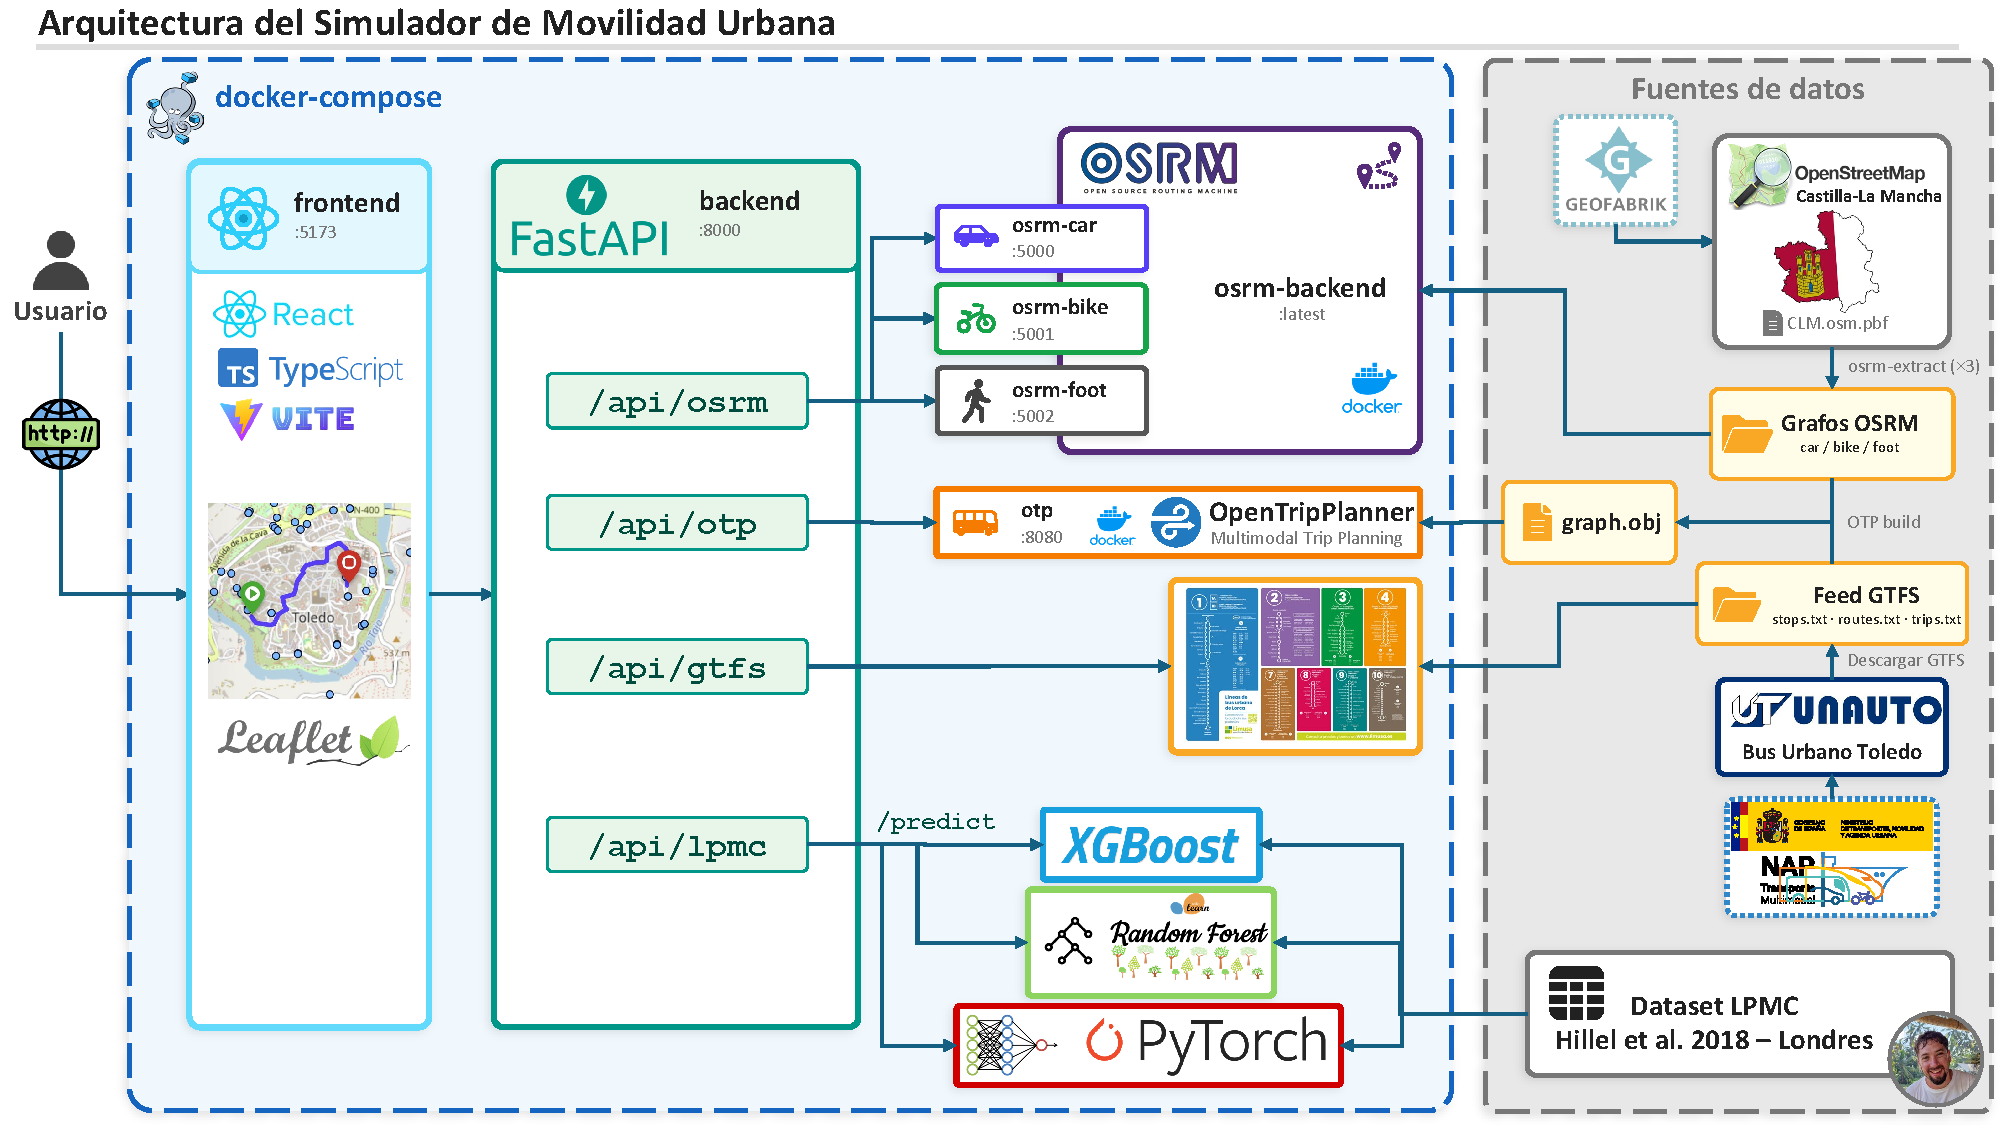
\includegraphics[width=\textwidth]{figs/ARQUITECTURA_pytorch_final.pdf}
  \caption{Arquitectura general del simulador de movilidad urbana.}
  \label{fig:arch_general}
\end{figure}

El frontend expone la interfaz cartográfica al usuario y delega en el backend el cálculo de rutas, la consulta de horarios GTFS y la inferencia modal. El backend integra cuatro routers diferenciados: \texttt{/api/osrm} para rutas viarias por perfil, \texttt{/api/otp} para itinerarios multimodales, \texttt{/api/gtfs} para información estática de la red de transporte, y \texttt{/api/lpmc} para la inferencia de elección modal. Cada router encapsula la lógica de comunicación con su servicio subyacente y expone al frontend una interfaz homogénea independiente de los detalles de cada protocolo.

% -------------------------------------------------------
\section{Infraestructura y orquestación}
\label{sec:arch_infra}
% -------------------------------------------------------

La infraestructura del sistema se define íntegramente en un fichero \texttt{docker-compose.yml} en la raíz del repositorio. El despliegue completo se obtiene con un único comando (\texttt{docker compose up -{}-build}), lo que elimina dependencias de entorno en la máquina anfitriona y garantiza reproducibilidad.

\begin{figure}[htbp]
  \centering
  % \includegraphics[width=0.92\textwidth]{figures/arch_docker.pdf}
  \missingfigure{Diagrama de servicios Docker Compose: frontend :5173, backend :8000, osrm-car :5001, osrm-bike :5002, osrm-foot :5003, otp :8080, y servicios de inicialización gtfs-init, osrm-setup y otp-build. Volúmenes montados en OSRM y OTP.}
  \caption{Servicios Docker Compose y puertos expuestos.}
  \label{fig:arch_docker}
\end{figure}

La Tabla~\ref{tab:servicios_docker} resume los servicios definidos, sus puertos y su función en el sistema.

\begin{table}[htbp]
  \caption{Servicios Docker Compose del simulador.}
  \label{tab:servicios_docker}
  \centering
  \begin{tabular}{llp{7cm}}
    \hline
    \textbf{Servicio} & \textbf{Puerto} & \textbf{Función} \\
    \hline
    \texttt{frontend}   & 5173 & Interfaz web React servida por Vite. \\
    \texttt{backend}    & 8000 & API FastAPI, orquestación y lógica de negocio. \\
    \texttt{osrm-car}   & 5001 & Motor OSRM con perfil de vehículo a motor. \\
    \texttt{osrm-bike}  & 5002 & Motor OSRM con perfil de bicicleta. \\
    \texttt{osrm-foot}  & 5003 & Motor OSRM con perfil peatonal. \\
    \texttt{otp}        & 8080 & OpenTripPlanner 2.x con grafo multimodal de Toledo. \\
    \hline
  \end{tabular}
\end{table}

Los servicios OSRM montan los grafos viarios preprocesados desde directorios locales mediante volúmenes Docker. OpenTripPlanner carga el grafo multimodal (\texttt{graph.obj}) generado a partir de los datos OSM de Castilla-La Mancha y el feed GTFS urbano de Toledo. Estos artefactos pesados se versionan mediante Git LFS (\textit{Large File Storage}), de modo que un clon del repositorio dispone de ellos sin necesidad de reconstruirlos. Para cubrir el caso de un clon sin LFS o de una actualización de los datos de origen, la orquestación incorpora además varios servicios de inicialización idempotentes que se ejecutan una sola vez antes de levantar el sistema: \texttt{gtfs-init} descomprime el feed GTFS, \texttt{osrm-setup} preprocesa los grafos viarios por perfil si faltan y \texttt{otp-build} construye el grafo de OTP si no está presente. El procedimiento completo, tanto automático como manual, se describe en el anexo~\ref{anx:despliegue}.

La razón por la que OSRM se instancia tres veces en lugar de usar un único servidor multiperfil es que la imagen oficial de OSRM no admite perfiles simultáneos: cada proceso solo puede servir el grafo con el que fue preprocesado. Esta limitación fue el detonante del cambio de la solución inicial basada en el servidor de demostración público, que únicamente ofrecía perfil de conducción, a la infraestructura local multiperfil descrita aquí.

% -------------------------------------------------------
\section{Backend: capa de orquestación}
\label{sec:arch_backend}
% -------------------------------------------------------

El backend está implementado con FastAPI sobre Python y se organiza en cuatro routers, cada uno responsable de un dominio funcional. La separación en routers permite desarrollar, probar y documentar cada integración de forma independiente. La Tabla~\ref{tab:endpoints_api} recoge los endpoints principales expuestos por cada router.

\begin{table}[htbp]
  \caption{Endpoints principales de la API REST del backend.}
  \label{tab:endpoints_api}
  \centering
  \begin{tabular}{llp{6.5cm}}
    \hline
    \textbf{Método} & \textbf{Ruta} & \textbf{Descripción} \\
    \hline
    POST & \texttt{/api/osrm/routes}                  & Rutas viarias multimodales (OSRM). \\
    POST & \texttt{/api/otp/routes}                   & Itinerario de transporte público (OTP). \\
    GET  & \texttt{/api/gtfs/stops}                   & Listado de paradas con filtro bbox. \\
    GET  & \texttt{/api/gtfs/routes}                  & Listado de líneas de la red. \\
    GET  & \texttt{/api/gtfs/routes/\{id\}}           & Detalle de ruta: paradas y trazado. \\
    GET  & \texttt{/api/gtfs/routes/\{id\}/schedule}  & Horarios de una línea por fecha. \\
    POST & \texttt{/api/lpmc/predict}                 & Inferencia de elección modal con el modelo activo. \\
    POST & \texttt{/api/lpmc/compare}                 & Inferencia simultánea con XGBoost, RF y DNN. \\
    POST & \texttt{/api/lpmc/debug-features}          & Vector de características antes/después del escalado. \\
    GET  & \texttt{/api/lpmc/models}                  & Modelos disponibles y variante por defecto. \\
    GET  & \texttt{/health}                           & Comprobación de disponibilidad. \\
    \hline
  \end{tabular}
\end{table}

El router \texttt{/api/osrm} recibe un par origen-destino con la lista de perfiles solicitados, consulta en paralelo las instancias OSRM correspondientes y devuelve al frontend las rutas con distancia, duración y geometría decodificada para su representación cartográfica.

El router \texttt{/api/otp} consulta el planificador multimodal y gestiona la paginación de itinerarios alternativos. La respuesta incluye el desglose por tramos (\textit{legs}), con tipo de modo, geometría, parada de inicio y fin, y agencia operadora cuando el tramo es de transporte público. Los itinerarios se ordenan por duración y se selecciona automáticamente el primero que incluya al menos un tramo de transporte público; si ninguno lo incluye, se devuelve el de menor duración.

El router \texttt{/api/gtfs} expone información estática de la red de transporte: listado de paradas con sus líneas asociadas, listado de rutas, detalle de ruta con paradas ordenadas y trazado geométrico, y resumen de horarios por fecha. Estos datos se leen directamente del feed GTFS descomprimido en el backend, sin depender de OpenTripPlanner, lo que permite consultar la red aunque el grafo OTP no esté disponible.

El router \texttt{/api/lpmc} recibe las coordenadas de origen y destino junto con el perfil sociodemográfico del viajero, construye el vector de variables de entrada al modelo consultando OSRM y OTP internamente, convierte las duraciones a horas para coincidir con las unidades del dataset de entrenamiento, aplica el escalado parcial y ejecuta la inferencia. El endpoint \texttt{/predict} usa el modelo activo; \texttt{/compare} ejecuta los tres modelos (XGBoost, Random Forest, DNN) sobre el mismo viaje y devuelve sus probabilidades comparadas; \texttt{/debug-features} expone el vector de características antes y después del escalado para validación del pipeline.

% -------------------------------------------------------
\section{Frontend: interfaz cartográfica}
\label{sec:arch_frontend}
% -------------------------------------------------------

El frontend está desarrollado con React, Vite y TypeScript. La aplicación se estructura en dos componentes principales: \texttt{App}, que concentra el estado global y la lógica de negocio del cliente, y \texttt{MapView}, que encapsula la representación cartográfica mediante React-Leaflet.

\texttt{App} gestiona los puntos de origen y destino, el modo de transporte activo, los resultados de rutas, la capa GTFS y el perfil de usuario para la inferencia. Las peticiones al backend se realizan con TanStack Query (\texttt{useQuery} y \texttt{useMutation}), que proporciona caché, gestión de estados de carga y reintento automático. El estado local de React es suficiente para el alcance del prototipo: no existe flujo de datos compartido entre componentes independientes que justifique una biblioteca adicional de gestión de estado.

\texttt{MapView} recibe el estado relevante como \textit{props} y se encarga exclusivamente de la renderización cartográfica: marcadores de origen y destino, polilíneas de ruta coloreadas según el modo activo, paradas GTFS con popups interactivos y segmentos OTP diferenciados visualmente entre tramos a pie y tramos en vehículo. Los segmentos de transporte público solo se muestran cuando el modo activo es \textit{transit}, evitando solapamientos visuales con las rutas viarias. La capa de fondo es configurable entre cuatro basemaps: carto-light (analítico, sin distracciones visuales), OpenStreetMap estándar (cartografía en color), OpenTopoMap (relieve con curvas de nivel) y satélite Esri (imágenes aéreas).

% -------------------------------------------------------
\section{Pipeline de inferencia modal}
\label{sec:arch_pipeline_inferencia}
% -------------------------------------------------------

La inferencia de elección modal es la operación más compleja del sistema porque requiere coordinar tres servicios externos de forma concurrente para construir el vector de entrada al modelo. La Figura~\ref{fig:pipeline_inferencia} ilustra el flujo completo.

\begin{figure}[htbp]
  \centering
  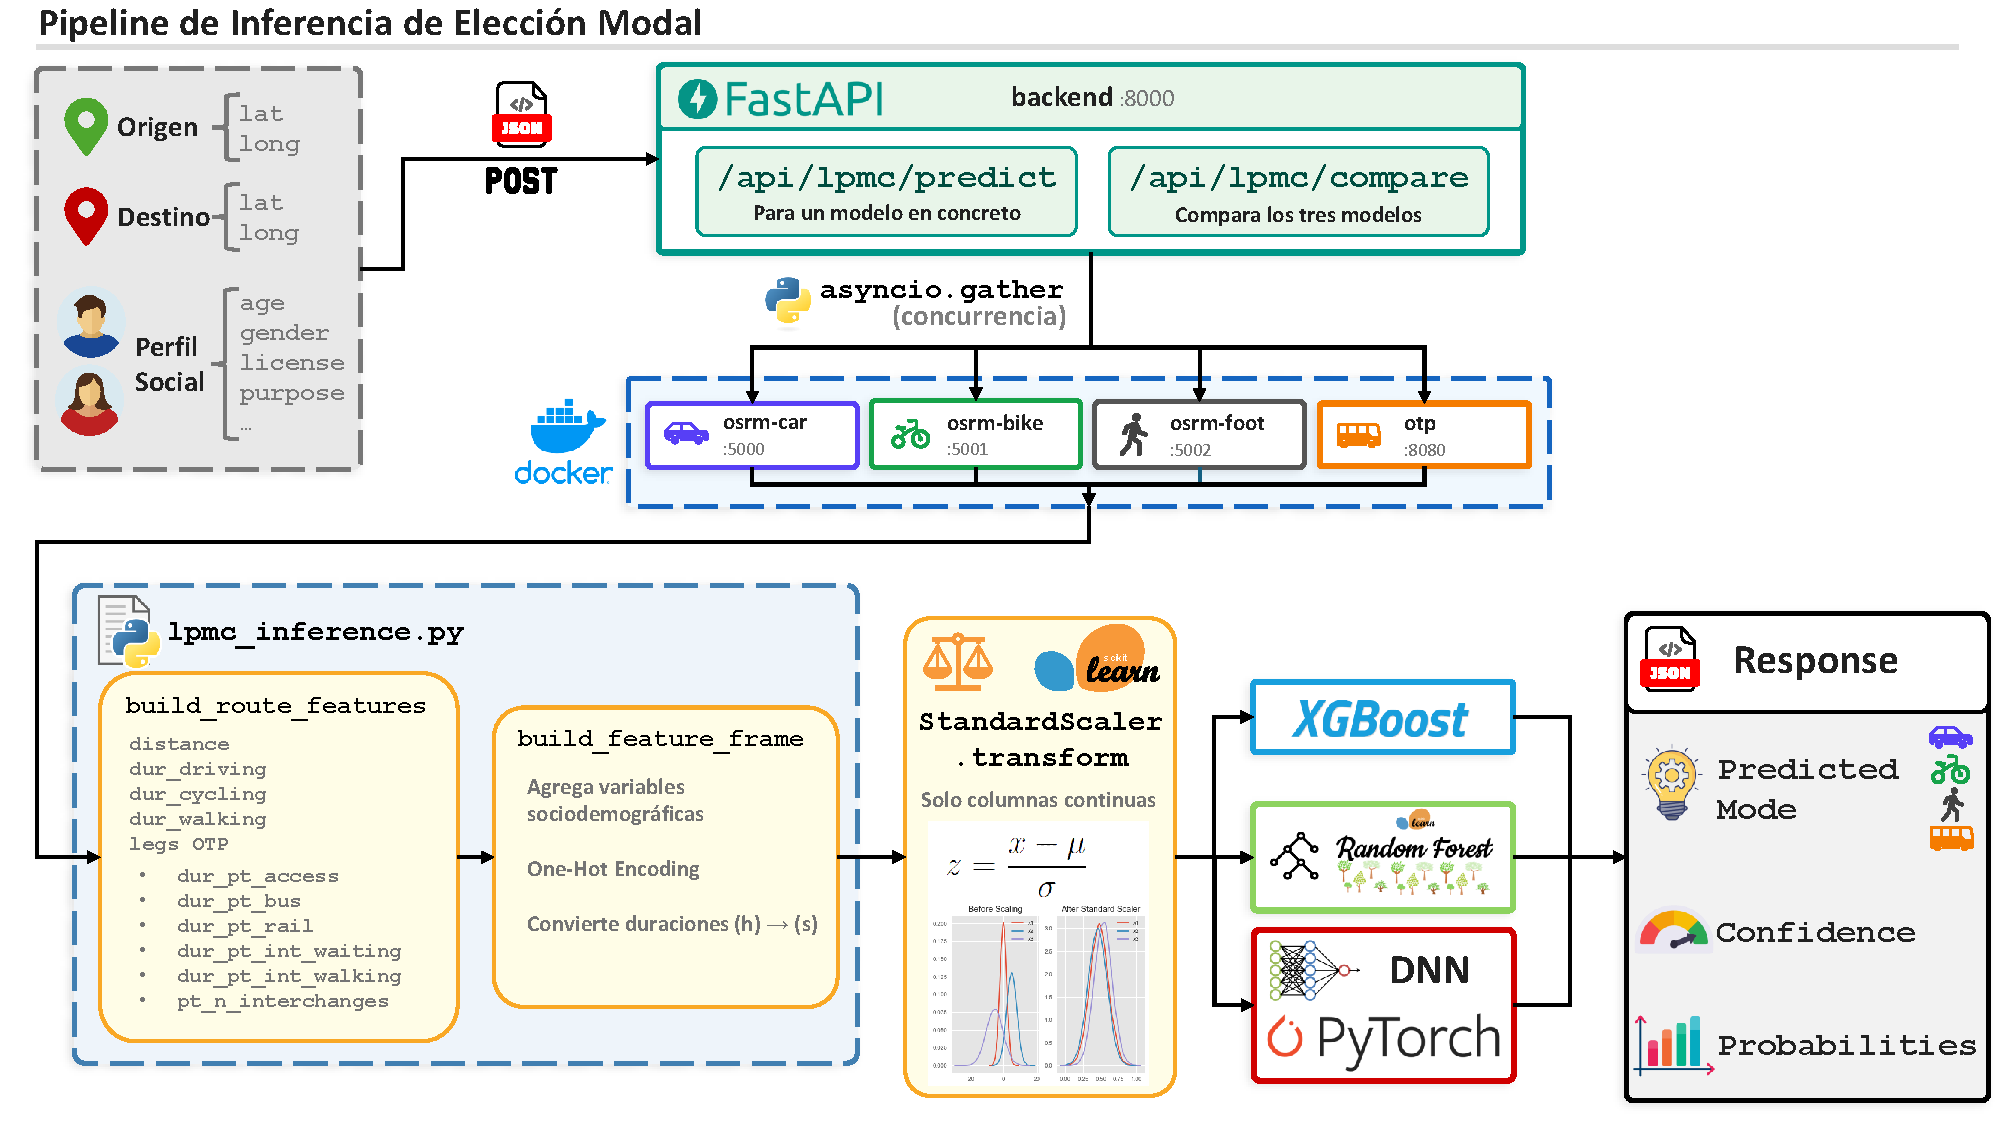
\includegraphics[width=\textwidth]{figs/PIPELINE_Inferencia.pdf}
  \caption{Pipeline de inferencia de elección modal.}
  \label{fig:pipeline_inferencia}
\end{figure}

Al recibir una petición \texttt{POST /api/lpmc/predict}, el backend lanza en paralelo cuatro consultas asíncronas mediante \texttt{asyncio.gather}: una a cada una de las tres instancias OSRM (conducción, bicicleta, a pie) y una a OpenTripPlanner. Con los resultados se construye el vector de características de ruta, se añaden las variables sociodemográficas del perfil recibido en la petición y se ensambla el vector completo de entrada al modelo.

Las variables de entrada al modelo proceden de tres fuentes diferenciadas: los tiempos y distancias por perfil de transporte calculados por OSRM, el desglose temporal del itinerario de transporte público proporcionado por OTP, y los datos sociodemográficos y contextuales que el usuario introduce en el formulario del panel lateral. El capítulo~\ref{ch:implementacion} detalla la construcción del vector de características y las transformaciones aplicadas.

Las variables continuas que presentaban distribución asimétrica en el conjunto de entrenamiento se normalizan con un escalado parcial aplicado solo a las columnas correspondientes, preservando las variables binarias y de conteo sin transformar. El modelo devuelve un vector de cuatro probabilidades correspondientes a los modos \textit{walk}, \textit{cycle}, \textit{pt} y \textit{drive}; el modo predicho es el de mayor probabilidad.

El modelo utilizado en \texttt{/predict} se elige mediante el parámetro opcional \texttt{model\_variant} de la propia petición; cuando no se indica, se recurre a la variable de entorno \texttt{LPMC\_MODEL\_VARIANT} (\texttt{xgb} por defecto), lo que mantiene la compatibilidad con clientes que no especifiquen el modelo. Ninguno de los tres modelos recibe \texttt{household\_id} como variable de entrada, ya que ese identificador de hogar no está disponible en tiempo de ejecución; su uso durante el entrenamiento se detalla en la sección~\ref{subsec:impl_lpmc_entrenamiento}.

% Decisiones técnicas movidas al capítulo 5 (implementación)

% % -------------------------------------------------------
% \section{Decisiones técnicas (ch5)}
% \label{sec:arch_decisiones}
% % -------------------------------------------------------

% A lo largo del desarrollo se tomaron varias decisiones de diseño que condicionan la arquitectura actual.

% \textbf{OSRM local frente al servidor de demostración.} La solución inicial utilizaba el demoserver público de OSRM, que solo proporciona el perfil de conducción. La imposibilidad de obtener tiempos de bicicleta y desplazamiento a pie, variables imprescindibles para el modelo LPMC, obligó a desplegar OSRM localmente con tres perfiles independientes. El coste es un mayor requisito de almacenamiento y memoria en tiempo de ejecución, compensado por la autonomía completa sobre los datos y la ausencia de límites de cuota.

% \textbf{Tres instancias OSRM en lugar de una.} La imagen oficial de OSRM no admite múltiples perfiles en un único proceso: cada instancia solo puede servir el grafo con el que fue preprocesada mediante \texttt{osrm-extract} y \texttt{osrm-partition}. La solución adoptada es desplegar tres contenedores independientes, cada uno con su grafo, mapeados a puertos distintos del host.

% \textbf{Fecha y hora fijas en OTP.} OpenTripPlanner calcula itinerarios en función de los calendarios de servicio del feed GTFS. Usar la fecha y hora reales introducía inconsistencias: en fines de semana o festivos el servicio es reducido o inexistente, lo que hacía que OTP devolviera itinerarios atípicos o ninguno. La solución adoptada es usar una fecha laborable fija (\texttt{2025-12-01}) y una hora de alta frecuencia de servicio (\texttt{12:00}), garantizando resultados representativos del servicio habitual.

% \textbf{Variante nohh del modelo LPMC.} El modelo original incluía \texttt{household\_id} como variable de entrada, lo que imposibilita su uso en inferencia ya que el simulador no tiene acceso a ese identificador. Se entrenó una variante alternativa excluyendo esa variable (\texttt{nohh}), que es la activa por defecto. La variante original se conserva como respaldo y el sistema puede alternar entre ambas mediante variable de entorno.

% \textbf{Colores de línea GTFS deterministas.} El feed GTFS de Toledo no incluye de forma consistente los campos \texttt{route\_color} y \texttt{route\_text\_color}. Para garantizar consistencia visual entre sesiones, el color de cada línea se deriva de forma determinista a partir del \texttt{route\_id} mediante una función de hash, de modo que la misma línea siempre se muestra con el mismo color independientemente del estado del servidor.

% \textbf{Carga perezosa de artefactos del modelo.} Los modelos (XGBoost, Random Forest, DNN) y sus escaladores se cargan desde disco la primera vez que se solicita cada variante y se mantienen en caché indexada por variante a nivel de módulo durante toda la vida del proceso. Esta estrategia de carga perezosa (\textit{lazy loading}) evita aumentar el tiempo de arranque del contenedor y garantiza que cada artefacto se carga exactamente una vez, independientemente del número de peticiones concurrentes.

% \textbf{Penalización de variables PT sin itinerario real.} Cuando OTP no encuentra un itinerario con transporte público, las variables de ruta PT (\texttt{dur\_pt\_access}, \texttt{dur\_pt\_bus}, \texttt{dur\_pt\_rail}, \texttt{pt\_n\_interchanges}) toman valor cero, lo que puede inducir al modelo a predecir \textit{pt} como modo mayoritario en trayectos sin servicio real. La solución, pendiente de implementar en el momento de escritura, consiste en asignar un valor de penalización alto a estas variables cuando OTP no devuelva un itinerario con al menos un tramo de transporte público.
\chapter{Implementación y resultados}
\label{ch:implementacion}

Este capítulo detalla el proceso de construcción del simulador: las decisiones técnicas concretas tomadas en cada componente, los problemas que surgieron durante el desarrollo así como la solución adoptada en cada caso, y los resultados del entrenamiento y evaluación de los modelos de elección modal.

El sistema implementado está disponible como código abierto en \url{https://github.com/ivanuclm/movilidad-urbana}, lo que permite su reproducción, extensión y reutilización en futuros trabajos de investigación, desarrollo o divulgación sobre movilidad urbana. El procedimiento de despliegue para reproducir el entorno local se detalla en el anexo~\ref{anx:despliegue}.


% -------------------------------------------------------
\section{Infraestructura de enrutado viario: OSRM}
\label{sec:impl_osrm}
% -------------------------------------------------------

\subsection{Origen y características del extracto OSM}
\label{subsec:impl_osrm_origen}

Open Source Routing Machine (OSRM) trabaja sobre un extracto de OpenStreetMap (OSM), un fichero binario con extensión \texttt{.osm.pbf} que contiene la geometría de calles, carreteras y caminos de un territorio junto con sus atributos de velocidad, sentido y accesibilidad por modo. Geofabrik \cite{GeofabrikDownloads} distribuye estos extractos por jerarquía geográfica, desde continentes hasta comunidades autónomas.

Se utilizó el extracto de Castilla-La Mancha al ser la región en la que se enmarca el proyecto, escogiendo Toledo como caso de estudio definitivo, tal como se detalla en la sección~\ref{sec:impl_otp}. OpenTripPlanner reutiliza el mismo extracto para la red viaria peatonal, por lo que un único fichero sirve a dos servicios del sistema. La Tabla~\ref{tab:osm_extractos} resume los extractos de OSM evaluados durante el desarrollo.

\begin{table}[H]
  \caption{Comparativa de extractos OSM disponibles en Geofabrik.}
  \label{tab:osm_extractos}
  \centering
  \begin{tabular}{lrl}
    \toprule
    \textbf{Extracto} & \textbf{Tamaño (.osm.pbf)} & \textbf{Uso en el proyecto} \\
    \midrule
    Castilla-La Mancha  & \textasciitilde{}98 MB     & Producción (OSRM y OTP) \\
    % Comunidad Valenciana & \textasciitilde{}131 MB     & Pruebas iniciales con feed EMT Valencia \\
    Comunidad de Madrid & \textasciitilde{}79 MB     & Pruebas con feed EMT Madrid \\
    España              & \textasciitilde{}1{,}3 GB  & Evaluado, descartado por tamaño \\
    Europa              & \textasciitilde{}32{,}0 GB & Descartado por tamaño \\
    \bottomrule
  \end{tabular}
\end{table}

\subsection{Evolución del despliegue}
\label{subsec:impl_osrm_evolucion}

El despliegue de OSRM pasó por tres iteraciones antes de conseguir la configuración definitiva.

\textbf{Fase 1: servidor de demostración oficial.} La primera implementación utilizó el servidor de demostración público del proyecto OSRM (\texttt{router.project-osrm.org}) \cite{OSRMDocs}. Este servidor ofrece acceso gratuito a la API de enrutado sin necesidad de infraestructura local y está pensado para pruebas rápidas de integración. El problema es que solo procesa el perfil de conducción independientemente del indicado en la URL \cite{OSRMIssue4034}; cambiar el perfil en la petición no tiene efecto, lo que hacía inviable la comparación multimodal que el simulador requiere.

\textbf{Fase 2: instancias públicas FOSSGIS.} Las instancias públicas mantenidas por FOSSGIS \cite{FOSSGISRouting} sí devuelven rutas diferenciadas por perfil mediante endpoints independientes (\texttt{/routed-car}, \texttt{/routed-bike}, \texttt{/routed-foot}), lo que permitió confirmar el funcionamiento multimodal y ajustar la integración del backend. El inconveniente es que estos servicios aplican limitaciones de uso (\textit{rate limiting}), presentan latencia variable y no permiten fijar la versión de los datos, lo que compromete la reproducibilidad.

\textbf{Fase 3: instancia local con Docker.} La solución definitiva fue desplegar OSRM localmente mediante la imagen oficial \texttt{osrm/osrm-backend} \cite{OSRMGitHub}, con un contenedor independiente por modo de transporte (conducción, bicicleta y a pie; el transporte público en autobús es responsabilidad de OpenTripPlanner). Esta arquitectura elimina la dependencia de servicios externos en tiempo de ejecución y garantiza reproducibilidad, control de versión y ausencia de límites de cuota. El preprocesado de los grafos, que originalmente se ejecutaba a mano, se automatizó posteriormente como un paso de inicialización de la orquestación Docker Compose (sección~\ref{sec:arch_infra}), de modo que el despliegue completo no requiere ningún comando manual. El procedimiento, tanto automático como los comandos equivalentes paso a paso, se recoge en el anexo~\ref{anx:despliegue}.


\subsection{Pipeline de preprocesado por perfil}
\label{subsec:impl_osrm_pipeline}

Para que OSRM pueda calcular rutas, el extracto \texttt{.osm.pbf} debe transformarse en una estructura de datos interna optimizada para ejecutar consultas y obtener el camino mínimo entre dos puntos del mapa. Este preprocesado se ejecuta una sola vez por perfil y solo hay que repetirlo si se actualiza el extracto de OSM.

Cada perfil define las reglas de movilidad del modo correspondiente: qué tipos de vía son accesibles, a qué velocidad y con qué restricciones de giro. Los tres archivos de perfil estándar (\texttt{car.lua}, \texttt{bicycle.lua} y \texttt{foot.lua}) están incluidos en la imagen oficial de Docker \texttt{osrm/osrm-backend} en \texttt{/opt/}, por lo que no es necesario descargarlos ni configurarlos externamente. Todas las etapas del preprocesado se ejecutan con esa misma imagen, lo que garantiza que el preprocesado sea reproducible en cualquier entorno de ejecución.

\begin{enumerate}
  \item \textbf{Extracción} (\texttt{osrm-extract}): lee el \texttt{.osm.pbf} y construye el grafo viario interno aplicando las reglas del perfil Lua indicado: qué vías son transitables, a qué velocidad y con qué restricciones. El resultado es el fichero \texttt{.osrm} junto con varios auxiliares de índice.
  \item \textbf{Particionado} (\texttt{osrm-partition}): divide el grafo en celdas jerárquicas para el algoritmo Multi-Level Dijkstra (MLD) \cite{Geisberger2008CH}. Esta partición es la que permite calcular rutas de larga distancia en milisegundos, al limitar la búsqueda a fronteras entre celdas en lugar de explorar el grafo completo.
  \item \textbf{Personalización} (\texttt{osrm-customize}): asigna los pesos finales de cada arista sobre la estructura de celdas anterior, produciendo el grafo listo para servir peticiones de ruta.
\end{enumerate}

Las tres etapas generan los ficheros \texttt{clm.osrm} y sus auxiliares, almacenados en directorios separados por perfil (\texttt{osrm-clm/car/}, \texttt{osrm-clm/bike/}, \texttt{osrm-clm/foot/}). Por su tamaño, estos artefactos se versionan mediante Git LFS (\textit{Large File Storage}), una extensión de Git que guarda los ficheros pesados fuera del historial principal y los referencia con punteros ligeros; así un clon del repositorio dispone de los grafos sin necesidad de regenerarlos. El procedimiento completo para reproducirlos se recoge en el anexo~\ref{anx:despliegue}.

El preprocesado completo de los tres perfiles sobre el extracto de Castilla-La Mancha tarda \todo{Revisar tiempos} aproximadamente 97 segundos en la máquina de desarrollo. Los artefactos generados ocupan en total unos 2,1~GB: el perfil de conducción produce 291~MB porque solo incorpora la red viaria accesible al tráfico rodado, mientras que los perfiles de bicicleta y peatonal alcanzan los 911~MB cada uno al incluir además senderos, caminos rurales y zonas de acceso restringido al tráfico.

\begin{figure}[htbp]
  \centering
  % \missingfigure{Diagrama del pipeline de preprocesado OSRM: \texttt{.osm.pbf} $\to$ \texttt{osrm-extract -p \{perfil\}.lua} $\to$ \texttt{osrm-partition} $\to$ \texttt{osrm-customize} $\to$ \texttt{osrm-routed -{}-algorithm mld}. Indicar que el proceso se repite de forma independiente para los tres perfiles (car, bike, foot), generando tres directorios de artefactos separados.}
  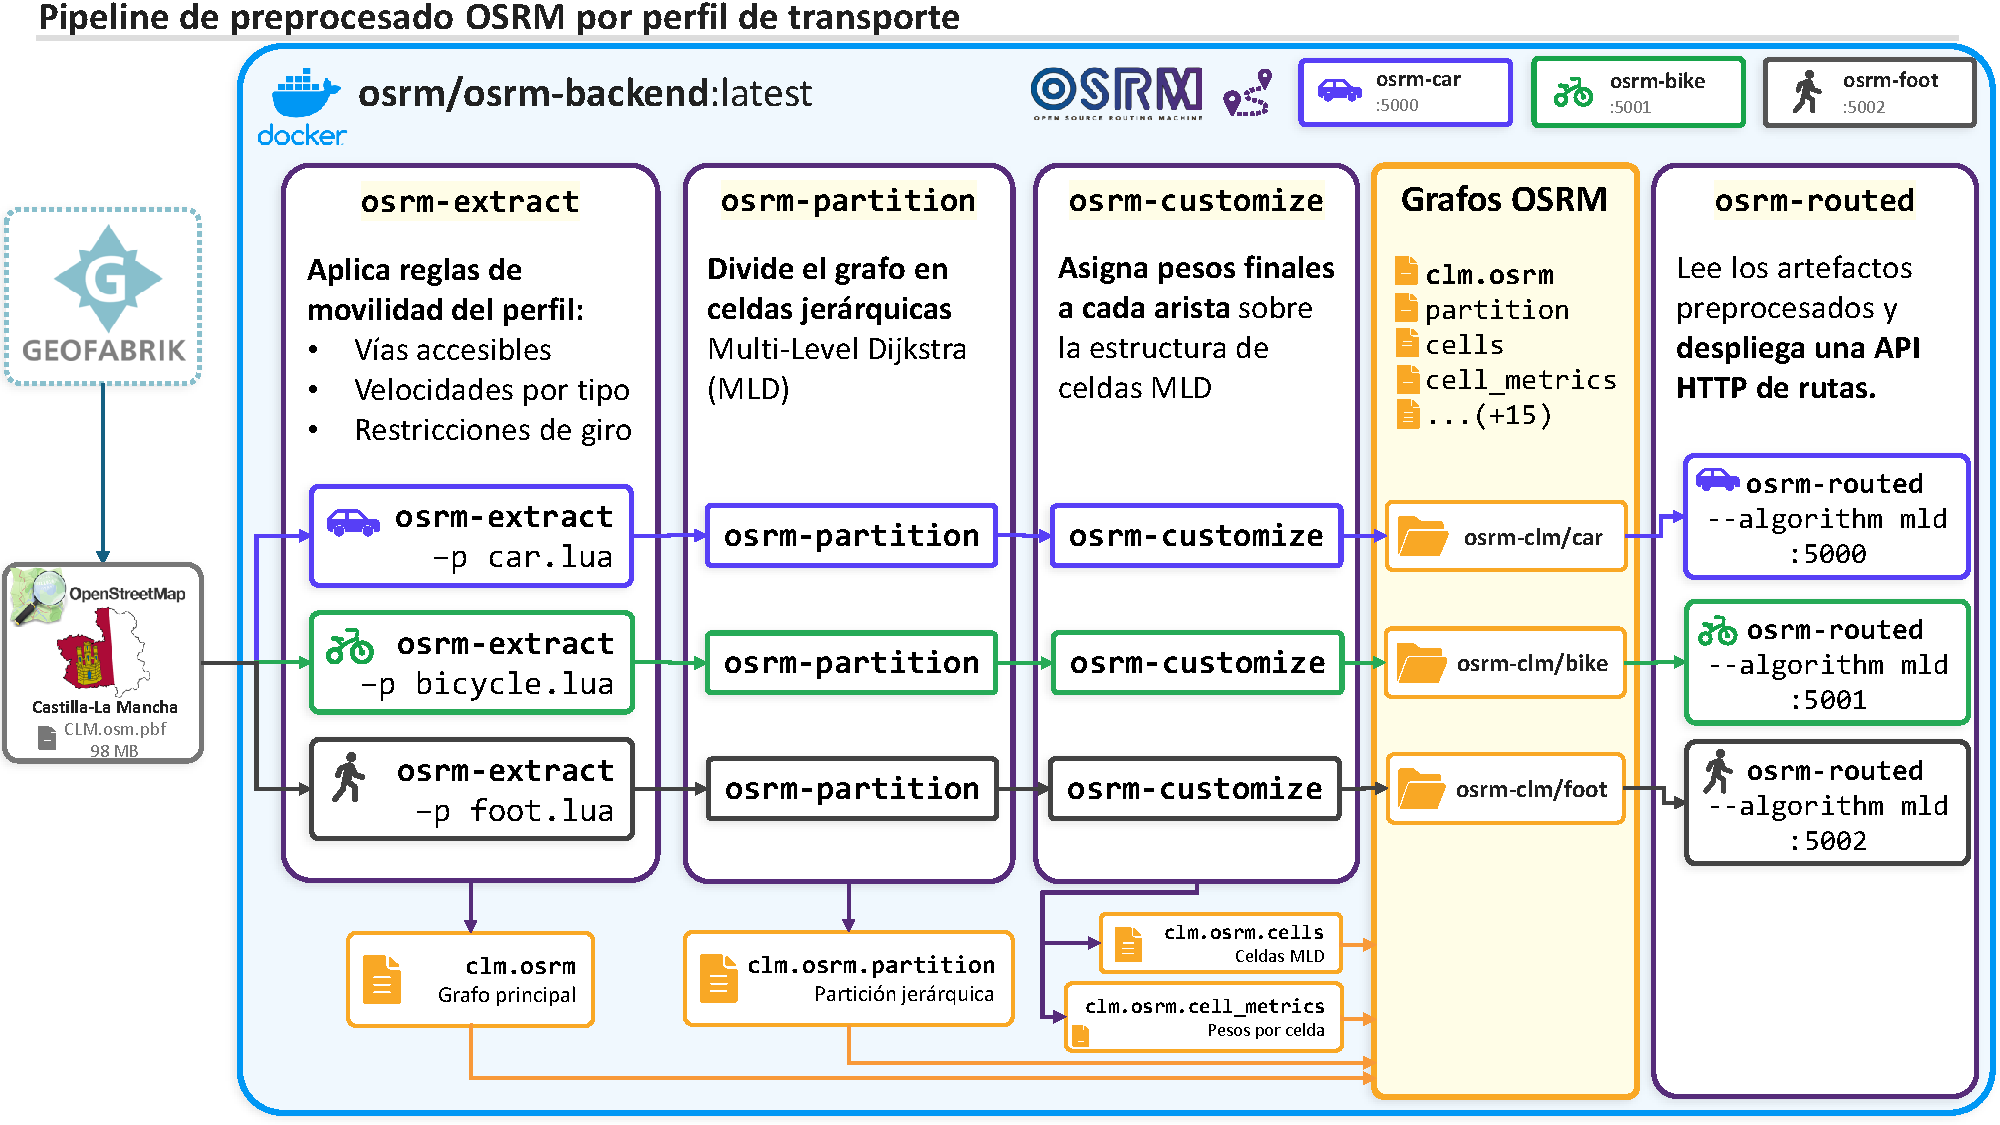
\includegraphics[width=1.0\textwidth]{figs/Pipeline_Preprocesado_OSRM.pdf}

  \caption{Pipeline de preprocesado OSRM por perfil de transporte.}
  \label{fig:osrm_pipeline}
\end{figure}

\subsection{Despliegue y verificación}
\label{subsec:impl_osrm_despliegue}

Cada uno de los tres contenedores OSRM ejecuta el servidor de enrutado sobre su grafo preprocesado con el algoritmo MLD (Figura~\ref{fig:osrm_pipeline}):
\begin{lstlisting}[language=bash]
osrm-routed --algorithm mld /data/clm.osrm
\end{lstlisting}

Los tres contenedores comparten imagen y comando de arranque. Cada uno monta el directorio de artefactos de su perfil (\texttt{osrm-clm/car}, \texttt{osrm-clm/bike}, \texttt{osrm-clm/foot}). Dentro de la red interna de Docker Compose, el proceso \texttt{osrm-routed} escucha siempre en el puerto 5000 en todos los contenedores, y el backend los referencia por nombre de servicio (\texttt{osrm-car}, \texttt{osrm-bike}, \texttt{osrm-foot}) en ese mismo puerto. Para verificar las instancias directamente desde el terminal del anfitrión, cada contenedor expone un puerto distinto hacia el exterior: 5001, 5002 y 5003, respectivamente para los perfiles de conducción, bicicleta y a pie. Se evita el puerto 5000 en el anfitrión porque en macOS lo ocupa por defecto un servicio del sistema (el receptor AirPlay), lo que impediría el arranque del contenedor; esta publicación de puertos solo se usa para depuración, ya que el backend se comunica con OSRM por la red interna.


Una respuesta válida devuelve \texttt{"code": "Ok"} junto con la distancia en metros, la duración en segundos y la geometría en formato polilínea~\cite{GooglePolyline}, una cadena de texto con la secuencia de coordenadas de la ruta, que el backend decodifica antes de enviarla al frontend. Si el grafo está incompleto o el perfil es incorrecto, OSRM devuelve \texttt{"code": "NoRoute"} o una ruta degradada, detectable al comparar visualmente los tres trazados en la interfaz.

\begin{code}[H]
\begin{lstlisting}[language=bash]
# osrm-car  (conduccion, localhost:5001)
curl "http://localhost:5001/route/v1/driving/-4.0356,39.8750;-4.0023,39.8602?overview=full"
# osrm-bike (bicicleta,  localhost:5002)
curl "http://localhost:5002/route/v1/cycling/-4.0356,39.8750;-4.0023,39.8602?overview=full"
# osrm-foot (peatonal,   localhost:5003)
curl "http://localhost:5003/route/v1/foot/-4.0356,39.8750;-4.0023,39.8602?overview=full"
\end{lstlisting}
\caption{Verificación de las tres instancias OSRM desde el terminal del anfitrión. El parámetro \texttt{overview=full} fuerza la devolución de la geometría completa de la ruta; sin él, OSRM devuelve una versión simplificada con menos puntos.}
\label{cod:osrm_verificacion}
\end{code}

La Figura~\ref{fig:osrm_rutas} muestra las tres rutas calculadas simultáneamente para el mismo par origen-destino: en azul, la ruta de conducción sigue las calles principales; en verde, la ruta de bicicleta prioriza carriles bici y calles tranquilas; en gris con línea discontinua, la ruta peatonal puede acceder a zonas restringidas al tráfico rodado. Los tres trazados ponen de manifiesto las distintas restricciones de cada perfil sobre la red viaria de Toledo.

\begin{figure}[H]
  \centering
  \includegraphics[width=1.0\textwidth]{figs/RutasSoloOSRM.jpeg}
  \caption{Rutas OSRM para los tres perfiles de transporte sobre Toledo.}
  \label{fig:osrm_rutas}
\end{figure}

% -------------------------------------------------------
\section{Planificación multimodal: OpenTripPlanner}
\label{sec:impl_otp}
% -------------------------------------------------------

\subsection{Fuente de datos GTFS y proceso de selección}
\label{subsec:impl_otp_gtfs}

OpenTripPlanner requiere dos fuentes de datos: un extracto viario OSM para modelar los tramos de acceso a pie, y un feed GTFS con el servicio programado del operador de transporte público para los tramos en vehículo. Al enmarcarse el proyecto en Castilla-La Mancha, la búsqueda de feed GTFS de bus urbano se orientó a la región desde el principio, con la ventaja de que el extracto OSM ya estaba disponible por su uso en OSRM (sección~\ref{subsec:impl_osrm_origen}). La fuente empleada fue el Punto de Acceso Nacional de Transporte Multimodal (NAP), gestionado por el Ministerio de Transportes y Movilidad Sostenible, que centraliza feeds GTFS de operadores de toda España \cite{NAPHome}. Aunque su cobertura a nivel nacional es amplia, la disponibilidad de feeds de transporte urbano en Castilla-La Mancha resultó muy limitada, como se detalla a continuación.

Las opciones disponibles en Castilla-La Mancha resultaron ser muy escasas. En Albacete solo figuraban servicios de operadores interurbanos como Alsa, sin datos de red urbana en el NAP. Guadalajara contaba con feeds del Consorcio de Transportes de Madrid (cercanías y autobuses interurbanos de la Comunidad de Madrid), pero sin red municipal propia. Cuenca tampoco disponía de feed urbano. La única opción urbana era Ciudad Real, cuyo feed, operado por AISA, incluía también Seseña, con paradas repartidas entre dos localidades separadas por más de 170~km; además, en ese momento no incluía geometría de rutas, requisito imprescindible para la representación cartográfica del servicio.

Ante la ausencia de un feed GTFS de Castilla-La Mancha válido, se evaluaron feeds de otras ciudades como candidatos alternativos para el proyecto. La EMT de Madrid \cite{NAPEMTMadrid}, con 4.914 paradas, 236 rutas y 87.137 viajes programados, sirvió de banco de pruebas para validar la integración de OTP con datos reales y desarrollar los endpoints de la capa estática del backend. El volumen del feed reveló además un problema de paginación: la API, que exige un límite explícito, devolvía solo las primeras 500 paradas por defecto, dejando la red visualmente incompleta. El límite se ajustó a 5.000, suficiente para Madrid y los feeds posteriores.

El feed GTFS elegido finalmente fue el de los autobuses urbanos de Toledo \cite{NAPToledoUrbano}. Con 268 paradas, 56 rutas y 87.751 viajes que cubren unos tres meses de servicio programado, tiene un tamaño ajustado al alcance del simulador, cubre el casco urbano, el polígono industrial y las urbanizaciones periféricas, e incluye geometría de rutas para su representación cartográfica. Como el feed no incluye tarifas, el coste del billete se introduce como parámetro en el panel lateral de la interfaz (de forma que pueda ser fijado por el analista en la simulación), junto al resto de variables del perfil de viajero, para su uso en la inferencia modal.
% El extracto OSM de Castilla-La Mancha ya disponible para OSRM servía también como base viaria para OTP, por lo que no fue necesario descargar ni preprocesar ningún fichero adicional.

\subsection{Periodo de validez del feed y selección de fecha}
\label{subsec:impl_otp_fecha}

Los feeds GTFS del NAP tienen un periodo de validez limitado; para el operador de Toledo (\texttt{GTFS\_Urbano\_Toledo\_2026}), los ficheros publicados cubren del 22 de febrero al 22 de mayo de 2026. Si la fecha de consulta cae fuera de ese rango, OTP no devuelve itinerarios de transporte público y el simulador queda sin oferta de bus sobre la que inferir. Durante el desarrollo se descargaron varias versiones del feed; en las primeras el operador figuraba como ``Autobuses urbanos Toledo'' y en posteriores había pasado a denominarse UNAUTO S.L. (Grupo Ruiz), aunque el formato de los ficheros GTFS se mantuvo en todas las versiones.

El mismo feed alimenta los dos subsistemas que consumen GTFS: el grafo de OTP (sección~\ref{subsec:impl_otp_grafo}) y la capa estática de horarios (sección~\ref{sec:impl_gtfs}), de modo que ambos comparten exactamente la misma ventana de validez. La fecha y la hora de consulta no se fijan en el código: se exponen mediante un control global en la interfaz, con un valor por defecto dentro del rango (\texttt{2026-05-21}, \texttt{12:00}) y acotado al intervalo válido del feed. Al ser un parámetro transversal a toda la simulación, este control único gobierna a la vez los itinerarios multimodales, los horarios de la red y el día y la hora del perfil de inferencia, evitando configuraciones contradictorias entre las distintas vistas; su ubicación y comportamiento en la interfaz se describen en la sección~\ref{subsec:impl_frontend_mapa}. El backend recibe la fecha y la hora en la petición y las traslada a OTP; cuando no se indican, aplica el valor por defecto.

Se fijó la hora por defecto a las 12:00 ya que se sitúa en la franja de mayor frecuencia de servicio y evita el horario nocturno, donde la oferta es reducida o inexistente.

OTP devuelve los instantes de paso en tiempo universal (epoch UTC) acompañados del desfase horario de la agencia (\texttt{agencyTimeZoneOffset}). El backend suma ese desfase antes de formatear las horas, de modo que los itinerarios se muestran en hora local de Toledo (Europe/Madrid), con el horario de verano resuelto automáticamente según la fecha consultada.

\subsection{Construcción del grafo multimodal}
\label{subsec:impl_otp_grafo}

El grafo se construye con un único comando Docker ejecutado sobre el directorio \texttt{otp-toledo/}, que debe contener el extracto OSM (\texttt{clm.osm.pbf}) y el feed GTFS (\texttt{GTFS\_Urbano\_Toledo\_2026.zip}):

\begin{lstlisting}[language=bash]
docker run --rm -v "otp-toledo:/var/opentripplanner" opentripplanner/opentripplanner:2.5.0 --build --save
\end{lstlisting}

OTP lee ambos ficheros y serializa el resultado en \texttt{graph.obj}: la red viaria OSM modela los tramos de acceso a pie a las paradas, y el feed GTFS aporta el servicio programado con horarios, paradas y geometría de las líneas. El proceso tarda unos minutos \todo{tiempos} y solo es necesario repetirlo cuando se actualiza el feed; el extracto OSM puede reutilizarse entre versiones. El comando anterior corresponde a la generación manual del grafo.

% Al igual que los grafos OSRM, el \texttt{graph.obj} no se versiona en el repositorio por su tamaño y debe generarse antes del primer despliegue.\todo{Completar anexo de despliegue con construcción del grafo OTP: comando --build --save y requisitos previos (OSM + GTFS)} Una vez disponible, OTP se lanza en modo de explotación (\texttt{--load --serve}) y queda accesible en el puerto 8080, exponiendo la API REST de planificación \cite{OTPRouteRequest}.

El \texttt{graph.obj} resultante (unos 120\,MB) se versiona mediante Git LFS para que el sistema arranque sin reconstrucción en un clon limpio. Como salvavidas, la orquestación incluye un servicio de inicialización idempotente (\texttt{otp-build}) que ejecuta \texttt{-{}-build -{}-save} únicamente si el grafo no está presente, de forma análoga a la compilación de los grafos OSRM. Una vez disponible, OTP se lanza en modo de explotación (\texttt{-{}-load -{}-serve}) y queda accesible en el puerto 8080, exponiendo la API REST de planificación \cite{OTPDocs}.



\subsection{Integración de itinerarios en el backend}
\label{subsec:impl_otp_integracion}

El router \texttt{/api/otp} del backend consulta OTP mediante peticiones HTTP a \texttt{/otp/routers/default/plan} y deserializa la respuesta para extraer los tramos (\textit{legs}) del itinerario seleccionado. OTP devuelve hasta cinco itinerarios alternativos. El criterio de selección automática es el siguiente: se elige el primero que incluya al menos un tramo de transporte público (modo distinto de \texttt{WALK}); si ninguno cumple esta condición, se devuelve el de menor duración total. El frontend permite paginar entre las alternativas mediante los botones ``Anterior'' y ``Siguiente'', que transmiten el índice del itinerario deseado al backend, garantizando que el vector de características para la inferencia se calcula siempre sobre el mismo itinerario que se visualiza.

Para cada tramo del itinerario seleccionado se devuelve: modo de transporte, distancia, duración, geometría decodificada, parada de inicio y fin, nombre de línea, agencia y horarios de salida y llegada en formato \texttt{HH:MM}. Para los tramos de transporte público se añade a la consulta el parámetro \texttt{showIntermediateStops}, que incorpora a la respuesta de OTP las paradas intermedias de cada tramo; con ellas el backend compone la secuencia ordenada completa de paradas del tramo, desde el embarque hasta el desembarque, anotando para cada una su nombre, coordenadas y hora de paso. Esta secuencia alimenta el diagrama de paradas del itinerario descrito en la sección~\ref{subsec:impl_frontend_legs}. La geometría, codificada en formato polyline, se decodifica en el frontend y se concatena para componer la traza completa del itinerario.


Cuando la distancia entre origen y destino es muy corta, o cuando no existe servicio de autobús entre los dos puntos en el horario fijado, OTP puede devolver como mejor itinerario una ruta completamente a pie, equivalente en tiempo y trayecto a la que ya proporciona OSRM con el perfil peatonal. En ese caso, si se construyese el vector de características de transporte público con los valores devueltos (tiempo de acceso cero, tiempo en bus cero, transbordos cero), el modelo podría asignar una probabilidad elevada al transporte público en trayectos sin servicio real. La solución adoptada, descrita en la sección~\ref{subsec:impl_backend_penalizacion}, consiste en detectar esta situación y sobrescribir las características de transporte público del vector con valores de penalización que llevan al modelo a descartar ese modo.

La Figura~\ref{fig:otp_itinerario} ilustra un itinerario multimodal típico en la interfaz del simulador: un tramo a pie inicial (trazado discontinuo en tono naranja oscuro) conecta el origen con la parada de embarque, un tramo en autobús (trazado continuo del color de la línea) cubre el recorrido principal, y un tramo a pie final lleva hasta el destino; las paradas del trayecto se marcan sobre el mapa con el color de su línea. En el panel lateral, una cabecera resume las horas de salida y llegada y la duración total, y bajo ella se despliega el detalle tramo a tramo: los tramos a pie como una línea de resumen y cada tramo en autobús como un diagrama vertical con todas sus paradas y la hora de paso por cada una. Al pulsar una parada del diagrama, el mapa se centra en ella y muestra su información, y los transbordos entre líneas se señalan de forma explícita.


\begin{figure}[H]
  \centering
%   \missingfigure{Captura de la interfaz mostrando un itinerario multimodal OTP sobre el mapa de Toledo: tramo a pie inicial (línea discontinua gris) desde el origen hasta la parada de embarque, tramo en autobús (línea continua de color) y tramo a pie final hasta el destino. En el panel lateral, desglose del itinerario con cada leg: modo, duración en minutos, paradas de inicio y fin, nombre de línea y horario de salida.}
    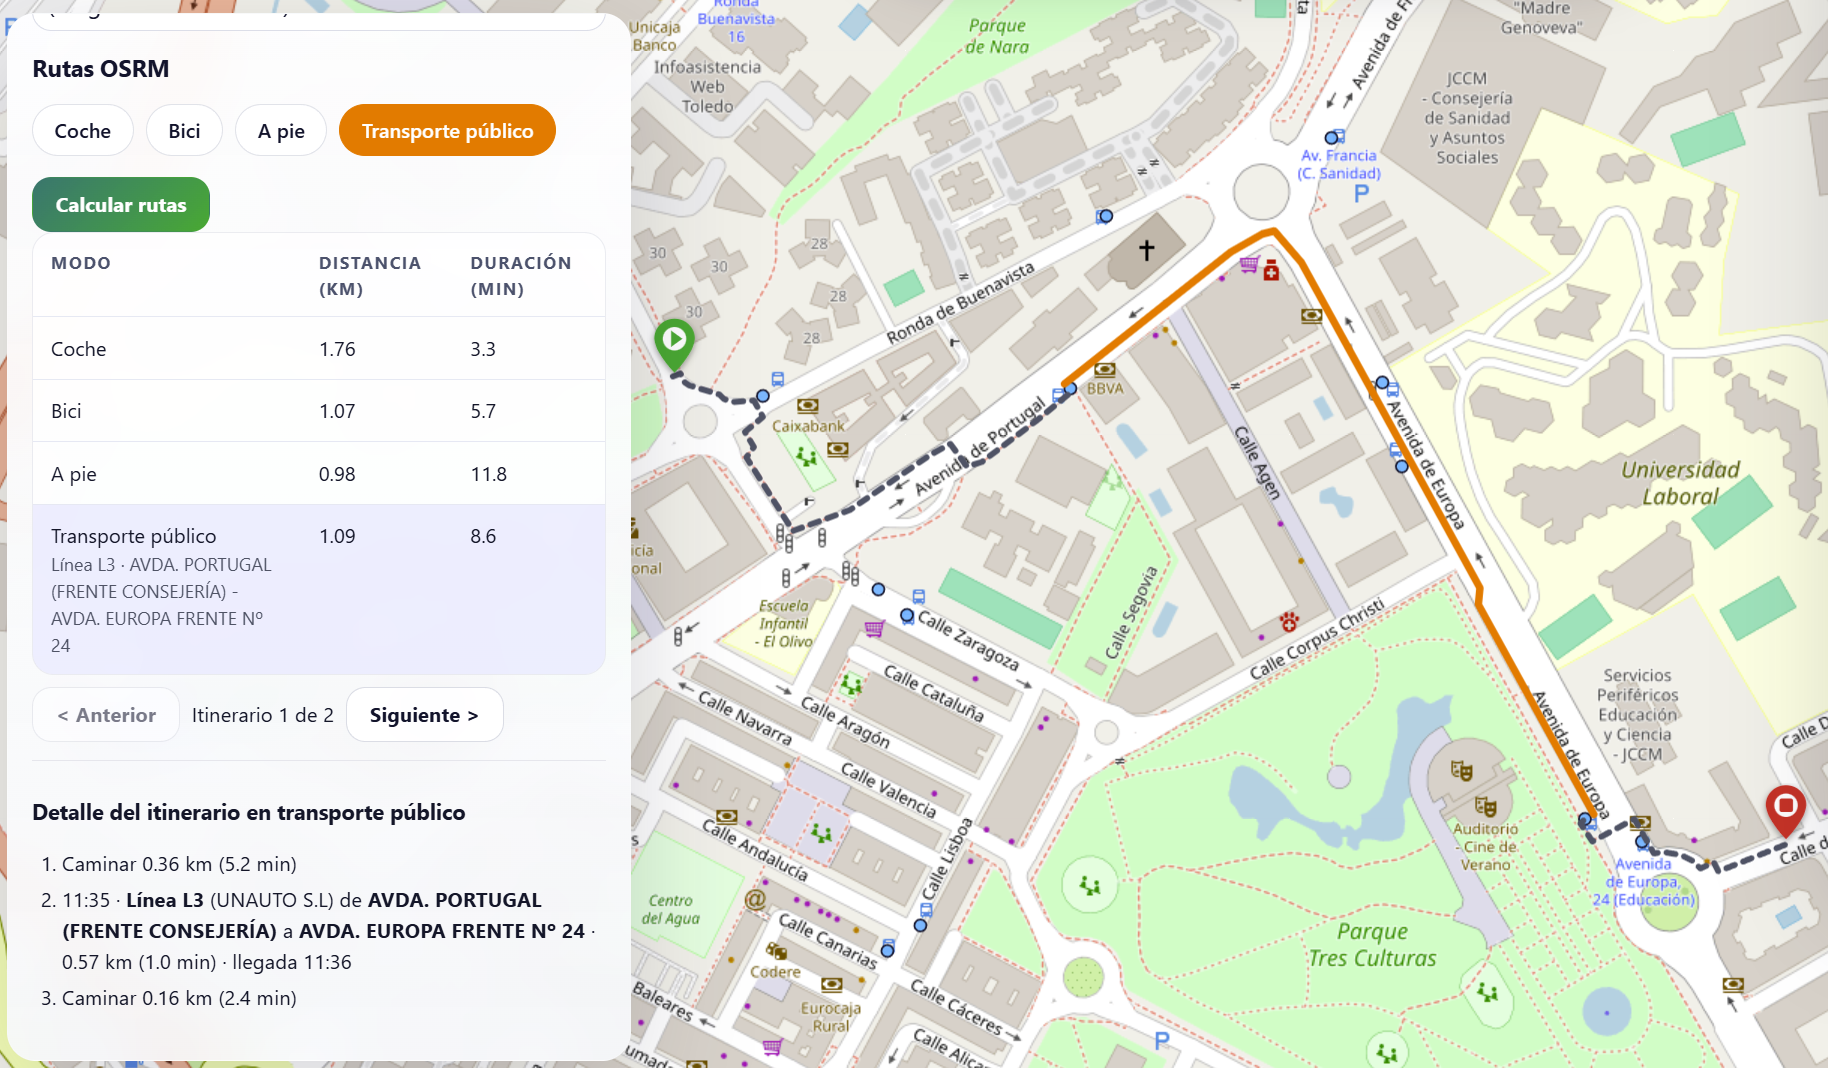
\includegraphics[width=1.0\textwidth]{figs/ItinerarioMultimodalZoom.png}
  \caption{Itinerario multimodal OTP con desglose de tramos en la interfaz.}
  \label{fig:otp_itinerario}
\end{figure}

% -------------------------------------------------------
\section{Integración del feed GTFS}
\label{sec:impl_gtfs}
% -------------------------------------------------------

\subsection{Arquitectura de la capa estática}
\label{subsec:impl_gtfs_arquitectura}

El router \texttt{/api/gtfs} expone la información estática de la red de autobús directamente a partir de los ficheros del feed GTFS, sin depender de OpenTripPlanner. Esto permite consultar y visualizar la red (paradas, líneas y horarios) de forma independiente del planificador.


El feed GTFS consiste en una colección de archivos de texto plano con extensión \texttt{.txt} y formato de valores separados por comas, empaquetados en un único archivo ZIP \cite{GTFSOverview}. En el arranque del servicio, el backend descomprime y carga en memoria con \texttt{pandas} los seis ficheros necesarios: \texttt{stops.txt} (paradas con coordenadas y nombre), \texttt{routes.txt} (líneas de la red), \texttt{trips.txt} (servicios programados por línea), \texttt{stop\_times.txt} (horarios de paso por cada parada), \texttt{shapes.txt} (geometría de los trazados) y \texttt{calendar\_dates.txt} (calendario de excepciones de servicio) \cite{GTFSReference}. Los DataFrames resultantes permanecen en memoria durante toda la vida del proceso.


Responder a preguntas como ``¿qué líneas pasan por esta parada?'' o ``¿cuál es el horario de una ruta para una fecha concreta?'' requiere cruzar varios de estos ficheros, tal como ilustra la Figura~\ref{fig:gtfs_joins}. Para obtener las líneas asociadas a una parada se encadenan tres cruces: \texttt{stops.txt} $\to$ \texttt{stop\_times.txt} $\to$ \texttt{trips.txt} $\to$ \texttt{routes.txt}. Para los horarios por fecha se añade el filtro de \texttt{calendar\_dates.txt}, que indica los días en que cada servicio está activo. Mantener todos los ficheros en memoria evita releer el feed completo en cada petición y elimina la necesidad de añadir una base de datos para datos que no cambian en tiempo de ejecución.

\begin{figure}[htbp]
  \centering
  \missingfigure{Diagrama de los seis ficheros GTFS como cajas (\texttt{stops}, \texttt{stop\_times}, \texttt{trips}, \texttt{routes}, \texttt{shapes}, \texttt{calendar\_dates}) con flechas que muestran los cruces por clave: \texttt{stops}\,--\,\texttt{stop\_times} (stop\_id), \texttt{stop\_times}\,--\,\texttt{trips} (trip\_id), \texttt{trips}\,--\,\texttt{routes} (route\_id), \texttt{trips}\,--\,\texttt{shapes} (shape\_id) y \texttt{trips}\,--\,\texttt{calendar\_dates} (service\_id). Resaltar la cadena stops$\to$stop\_times$\to$trips$\to$routes que resuelve ``líneas por parada''.}
  \caption{Cruces entre los ficheros del feed GTFS para resolver las consultas de la capa estática.}
  \label{fig:gtfs_joins}
\end{figure}

\subsection{Endpoints disponibles}
\label{subsec:impl_gtfs_endpoints}

La capa GTFS expone cuatro endpoints que cubren las operaciones necesarias para la visualización cartográfica y la consulta de la red:

\begin{itemize}
   \item \textbf{Listado de paradas} (\texttt{GET /api/gtfs/stops}): devuelve todas las paradas del feed con identificador, nombre, coordenadas y líneas asociadas. Acepta un parámetro \texttt{limit} (5.000 por defecto, suficiente para el feed de Toledo con 268 paradas) y un filtro de bounding box opcional para restringir el resultado al área visible en el mapa.

  \item \textbf{Listado de rutas} (\texttt{GET /api/gtfs/routes}): catálogo completo de líneas con identificador, nombre corto, nombre largo y atributos de color cuando están disponibles en el feed.

  \item \textbf{Detalle de ruta} (\texttt{GET /api/gtfs/routes/\{route\_id\}}): dado el identificador de una línea, devuelve la secuencia ordenada de paradas y la geometría del \textit{shape} asociado para su representación cartográfica.

\item \textbf{Horarios por fecha} (\texttt{GET /api/gtfs/routes/\{route\_id\}/schedule}): dado un identificador de ruta y una fecha especificada mediante el parámetro de consulta \texttt{date} (es decir, \texttt{?date=YYYY-MM-DD}), devuelve los servicios programados agrupados por dirección, con primera y última salida y listado completo de horarios. Al igual que con OTP (sección~\ref{subsec:impl_otp_fecha}), la interfaz usa una fecha fija dentro del rango de validez del feed en lugar de la fecha del sistema. Cualquier fecha posterior al rango de validez devuelve cero servicios.
\end{itemize}


\subsection{Coloración de líneas y agrupación por sentido}
\label{subsec:impl_gtfs_color}

El feed GTFS de Toledo incluye en \texttt{routes.txt} un color por línea (campos \texttt{route\_color} y \texttt{route\_text\_color}), que la interfaz utiliza directamente para mostrar cada línea con el color oficial del operador. Si un feed no incluye esos campos, la función \texttt{routeColor()} genera un color de reserva a partir del nombre corto de la línea: transforma el texto en un número entero y lo reduce módulo 360 para elegir un tono; la saturación y la luminosidad se mantienen fijas (70\,\% y 35\,\%, respectivamente) para que el color resultante tenga siempre contraste suficiente con el texto blanco superpuesto. Como un mismo nombre produce siempre el mismo número, cada línea conserva su color entre ejecuciones. El Código~\ref{cod:gtfs_color} recoge ambas funciones.

\begin{lstlisting}[language=Java, caption={Color de línea: feed GTFS como fuente primaria y hash determinista como respaldo.}, label={cod:gtfs_color}]
function hslForKey(key: string): string {
  let h = 0;
  for (let i = 0; i < key.length; i++) h = (h * 31 + key.charCodeAt(i)) | 0;
  return `hsl(${Math.abs(h) % 360}, 70%, 35%)`;
}
function routeColor(r: { color?: string | null; short_name?: string | null; id: string }): string {
  if (r.color) return `#${r.color}`;
  return hslForKey(r.short_name || r.id);
}
\end{lstlisting}

Este criterio de color se aplica de forma homogénea en toda la interfaz: en las etiquetas de línea del catálogo y del panel de rutas, en las etiquetas de las paradas, en el diagrama de paradas y en el trazado de la línea sobre el mapa. Algunas líneas del feed de Toledo son de color blanco (por ejemplo, la L14), y parecería invisible sobre el fondo claro de los paneles y del mapa. Para evitarlo, la función \texttt{isLightColor()} mide cuán claro es un color a partir de sus componentes de rojo, verde y azul y, si supera un umbral cercano al blanco, le añade un contorno oscuro.

El feed de Toledo contiene 56 entradas en \texttt{routes.txt} pero solo 25 líneas distintas, ya que el operador registra cada sentido y variante de recorrido como un \texttt{route\_id} independiente con el mismo \texttt{route\_short\_name}. La interfaz agrupa esas entradas por nombre corto en un diccionario (\texttt{routeSiblingsByShortName}), de modo que el catálogo muestra una sola entrada por línea. Cuando el usuario selecciona una línea, el sentido activo se deduce de la posición del \texttt{route\_id} elegido dentro del grupo de variantes; así, al pulsar la etiqueta de una parada en el mapa (que conoce el \texttt{route\_id} exacto del servicio que pasa por ella) se activa directamente el sentido correcto, sin lógica adicional.

La Figura~\ref{fig:gtfs_paradas} muestra el panel Red GTFS. El catálogo se organiza en un acordeón donde cada fila representa una línea física con su badge coloreado y nombre largo. Al expandir una entrada con varios sentidos, aparece una sublista con las variantes (sentidos) de la línea y el identificador activo resaltado mediante un borde lateral de su color. El panel muestra además un diagrama vertical de paradas inspirado en los paneles de andén: una barra vertical del color de la línea, con las terminales como puntos rellenos, las paradas intermedias como aros huecos y la parada de referencia resaltada en azul. Al pulsar sobre el nombre de una parada, el mapa ejecuta un desplazamiento animado (\texttt{flyTo}) hasta esa posición. Una tabla de salidas agrupada por hora completa la información de la ruta seleccionada; las salidas se muestran siempre para la fecha activa, atenuando las anteriores a la hora seleccionada en el control global, resaltando en azul las posteriores y en negrita la próxima salida. Si la línea no circula el día elegido, se sustituye la tabla por un aviso que indica los días en que sí presta servicio. De este modo el panel no necesita sus propios selectores de día: la fecha y la hora provienen del control global descrito en la sección~\ref{subsec:impl_otp_fecha}.



\begin{figure}[H]
  \centering
  \missingfigure{Panel Red GTFS: a la izquierda, el acordeón con la línea seleccionada desplegada mostrando el diagrama vertical de paradas y la tabla de horarios agrupada por hora (con las salidas pasadas atenuadas y la próxima resaltada); a la derecha, el trazado de la línea sobre el mapa de Toledo con sus paradas coloreadas.}
  \caption{Panel GTFS con acordeón de líneas, diagrama de paradas y horarios.}
  \label{fig:gtfs_paradas}
\end{figure}

% -------------------------------------------------------
\section{Implementación del backend FastAPI}
\label{sec:impl_backend}
% -------------------------------------------------------

\subsection{Estructura modular}
\label{subsec:impl_backend_estructura}

El backend está implementado con FastAPI sobre Python y organizado en módulos por responsabilidad. Un directorio \texttt{api/} contiene los cuatro routers (\texttt{routes\_osrm.py}, \texttt{routes\_otp.py}, \texttt{routes\_gtfs.py}, \texttt{routes\_lpmc.py}); un directorio \texttt{services/} contiene la lógica de negocio desacoplada de la capa HTTP (\texttt{osrm\_client.py}, \texttt{lpmc\_inference.py}); y el módulo raíz \texttt{main.py} monta los routers y habilita CORS (\textit{Cross-Origin Resource Sharing}), el mecanismo que autoriza al navegador a que la interfaz web, servida desde un puerto distinto, consuma la API del backend. Los endpoints expuestos por cada router se recogen en la Tabla~\ref{tab:endpoints_api} del capítulo~\ref{ch:arquitectura}.

La separación en módulos permite desarrollar, probar y documentar cada router de forma independiente. FastAPI genera documentación OpenAPI automática en \texttt{/docs} que refleja el estado actual de los endpoints en tiempo real, lo que facilitó la verificación del contrato de cada integración durante el desarrollo sin necesidad de un cliente HTTP externo.

\begin{figure}[htbp]
  \centering
  \missingfigure{Captura de la documentación OpenAPI automática (\texttt{/docs}) del backend FastAPI, mostrando los cuatro grupos de endpoints (/api/osrm, /api/otp, /api/gtfs, /api/lpmc) con sus rutas, métodos HTTP y esquemas de petición y respuesta.}
  \caption{Documentación OpenAPI generada automáticamente por FastAPI.}
  \label{fig:fastapi_docs}
\end{figure}

\subsection{Router OSRM: consultas multiperfil}
\label{subsec:impl_backend_osrm}

El router \texttt{/api/osrm/routes} acepta un par origen-destino y una lista de perfiles solicitados, y lanza las consultas a los tres contenedores OSRM en paralelo mediante \texttt{asyncio.gather}. La paralelización reduce la latencia total al tiempo de la consulta más lenta en lugar de la suma de las tres, lo que es especialmente útil cuando se solicitan los tres perfiles a la vez. Para cada perfil, el backend recibe la distancia en metros, la duración en segundos y la geometría en formato polyline, decodifica esta última en una lista de coordenadas \texttt{[lat, lon]} lista para Leaflet, y convierte las duraciones de segundos a horas antes de construir el vector de características, ya que el dataset LPMC almacena todas las duraciones en esa unidad.

\subsection{Router OTP: itinerarios multimodales}
\label{subsec:impl_backend_otp}

El router \texttt{/api/otp/routes} consulta el endpoint de planificación de OTP, gestiona la selección de itinerario (automática o por índice explícito recibido desde el frontend) y transforma la respuesta de OTP a un formato propio y homogéneo de tramos, más sencillo de consumir por el frontend. Para cada tramo del itinerario seleccionado se devuelve: modo de transporte, distancia, duración, geometría decodificada desde polyline, parada de inicio y fin, nombre de línea, agencia y horarios de salida y llegada. La geometría de cada tramo se concatena para formar la traza completa del itinerario, que el frontend divide y renderiza por segmentos según el modo.

\subsection{Penalización de itinerarios sin transporte público real}
\label{subsec:impl_backend_penalizacion}

Cuando OTP devuelve un itinerario compuesto exclusivamente por un tramo a pie, sin ningún tramo de transporte público, las características de transporte público del vector de entrada (tiempo de acceso a la parada, tiempo en el vehículo, tiempo de espera y de transbordo, y número de transbordos) tomarían valores próximos a cero. El problema es que esos mismos valores bajos caracterizan en el dataset a un transporte público rápido y directo, por lo que el modelo podría asignar una probabilidad elevada al transporte público en un trayecto donde en realidad no hay servicio. El caso se detectó durante las pruebas de integración del módulo de inferencia: en trayectos cortos en los que la opción más rápida era ir a pie, OTP devolvía ese único tramo como mejor itinerario y la inferencia resultaba engañosa.

Para evitarlo, el backend comprueba si el itinerario contiene algún tramo de transporte público. Si no es así, sobrescribe las seis características de transporte público (\texttt{dur\_pt\_access}, \texttt{dur\_pt\_bus}, \texttt{dur\_pt\_rail}, \texttt{dur\_pt\_int\_waiting}, \texttt{dur\_pt\_int\_walking} y \texttt{pt\_n\_interchanges}) con un valor situado en el extremo superior de su distribución. En concreto, a cada característica se le asigna el valor que, tras el escalado estándar (\texttt{StandardScaler}) del modelo, queda cinco desviaciones típicas por encima de la media de entrenamiento: es decir, $\mu + 5\sigma$, tomando la media $\mu$ y la desviación típica $\sigma$ que el escalador aprendió de esa característica. De este modo el modelo percibe un transporte público con tiempos y transbordos extremos, prácticamente inviable, y descarta esa opción sin necesidad de modificar su arquitectura ni el número de variables de entrada.

De forma análoga, en trayectos muy cortos (menos de 500~m en línea recta) el backend añade un recargo de tiempo al coche, que representa el aparcamiento y el acceso al vehículo. Sin él, el modelo tendería a elegir el coche siempre que su tiempo de conducción fuese menor, ignorando que para distancias tan cortas el sobrecoste de aparcar hace más razonable ir a pie. Ambas correcciones son ejemplos de conocimiento experto inyectado en las entradas del modelo; el análisis de cómo responde cada modelo a la penalización y la justificación de este enfoque se abordan en la sección~\ref{subsec:impl_lpmc_entrenamiento}.

\subsection{Router LPMC: inferencia modal y descubrimiento de modelos}
\label{subsec:impl_backend_lpmc}

El router \texttt{/api/lpmc} centraliza la lógica de inferencia de elección modal y el acceso a los modelos entrenados. A diferencia de los routers de enrutado, que delegan el cálculo en servicios externos (OSRM y OTP), este router ejecuta la predicción de forma local sobre los artefactos serializados en \texttt{lpmc/models/}. Expone cuatro endpoints:

\begin{itemize}
  \item \textbf{Predicción con modelo seleccionable} (\texttt{POST /api/lpmc/predict}): recibe el par origen-destino, el índice del itinerario OTP seleccionado, el perfil de usuario y, de forma opcional, el identificador de variante de modelo (\texttt{model\_variant}). Si no se especifica, se usa la variable de entorno \texttt{LPMC\_MODEL\_VARIANT} como predeterminado, manteniendo la compatibilidad con scripts externos que no pasen el parámetro. La respuesta incluye la probabilidad de cada uno de los cuatro modos (a pie, bicicleta, transporte público y coche), el modo más probable y su probabilidad, el vector de características de ruta (con las penalizaciones aplicadas si el trayecto resultó ser solo a pie) y varios metadatos del modelo: la ruta del artefacto, el indicador \texttt{pt\_available} (verdadero cuando el itinerario contiene al menos un tramo de transporte público) y el indicador de trayecto corto.

  \item \textbf{Comparación de modelos disponibles} (\texttt{POST /api/lpmc/compare}): ejecuta la predicción con cada variante en secuencia y devuelve un diccionario con los resultados de cada una. La ejecución es secuencial, no concurrente: a diferencia de las consultas a OSRM y OTP (que esperan respuestas de red y se benefician de la concurrencia), la inferencia es un cálculo intensivo en CPU que el intérprete de Python ejecuta en un único hilo, por lo que lanzarla en paralelo no aceleraría el proceso. La latencia adicional es aceptable, ya que el usuario activa la comparación de forma explícita, al margen del flujo de cálculo principal.

  \item \textbf{Depuración del vector de características} (\texttt{POST /api/lpmc/debug-features}): devuelve el vector completo ensamblado por \texttt{\_build\_feature\_frame()}, con los valores crudos y escalados. Facilita verificar que las variables de ruta calculadas a partir de OSRM y OTP se encuentran en el rango esperado por el dataset LPMC, y fue la herramienta principal para diagnosticar los errores de unidades descritos en la sección~\ref{subsec:impl_lpmc_entrenamiento}.

  \item \textbf{Descubrimiento de modelos disponibles} (\texttt{GET /api/lpmc/models}): escanea \texttt{lpmc/models/} buscando pares de ficheros \texttt{\{nombre\}\_lpmc.joblib} y \texttt{\{nombre\}\_lpmc\_scaler.joblib}. Devuelve la lista de variantes disponibles y la variante predeterminada según \texttt{LPMC\_MODEL\_VARIANT}. Este mecanismo permite añadir un modelo entrenado externamente al directorio y que la interfaz lo detecte en la siguiente petición, sin necesitar reiniciar ningún contenedor.
\end{itemize}

Dos detalles transversales completan el router. Primero, el identificador de variante recibido del exterior se valida con una expresión regular (\texttt{\textasciicircum[a-z0-9\_]\{1,32\}\$}), que solo admite letras minúsculas, dígitos y guiones bajos; con ello se evita que un valor manipulado se interprete como una ruta de fichero arbitraria al construir el nombre del artefacto a cargar. Segundo, los modelos se cargan de forma diferida y se conservan en una caché en memoria: la primera predicción con una variante asume el coste de leer y deserializar su artefacto desde disco, y las siguientes lo reutilizan sin volver a leerlo.

\subsection{Resolución de rutas y portabilidad}
\label{subsec:impl_backend_docker}

El backend necesita localizar en disco los datos del feed GTFS y los artefactos de los modelos. En lugar de codificar rutas absolutas, que dependerían del equipo y del sistema operativo concretos, cada módulo deriva la ruta que necesita a partir de su propia ubicación mediante la biblioteca estándar \texttt{pathlib}. Por ejemplo, la función auxiliar \texttt{\_project\_root()} del módulo de inferencia evalúa \texttt{Path(\_\_file\_\_).resolve().parents[4]}, que asciende cuatro niveles desde el fichero del módulo hasta la raíz del repositorio; desde ahí se compone la ruta a \texttt{lpmc/models/}. Este enfoque es portable entre el entorno de desarrollo (Windows) y el contenedor de ejecución (Linux) porque \texttt{pathlib} abstrae el separador de directorios propio de cada sistema y las rutas se calculan siempre de forma relativa a la posición del código, no a un punto de montaje fijo. La orquestación de los contenedores y el montaje del repositorio en ellos se describen en la sección~\ref{sec:arch_infra}.


% -------------------------------------------------------
\section{Implementación del frontend}
\label{sec:impl_frontend}
% -------------------------------------------------------

\subsection{Tecnologías y estructura}
\label{subsec:impl_frontend_tech}

El frontend está desarrollado con React 18, Vite y TypeScript. Vite proporciona recarga en caliente instantánea durante el desarrollo y genera el bundle de producción con división de código automática. TypeScript añade comprobación estática de tipos, especialmente útil al manejar las estructuras de datos complejas que devuelven los endpoints del backend: itinerarios OTP con desglose por tramos, respuestas GTFS con múltiples entidades relacionadas y vectores de probabilidades de los tres modelos. Leaflet se integra a través de React-Leaflet como librería cartográfica, y los iconos de la interfaz se proporcionan mediante Lucide React, una biblioteca de iconos SVG que no introduce dependencias adicionales en tiempo de ejecución.

La aplicación está estructurada en dos componentes principales, \texttt{App} y \texttt{MapView}, descritos en la sección~\ref{sec:arch_frontend}. Esta separación, en la que \texttt{MapView} recibe todos sus datos como \textit{props} y no mantiene estado propio, simplificó el desarrollo incremental de la capa cartográfica de forma independiente al resto de la lógica.

\subsection{Diseño de la interfaz: rail lateral y paneles}
\label{subsec:impl_frontend_ui}

La interfaz sigue un esquema inspirado en Google Maps: el mapa ocupa todo el área de la ventana del navegador como fondo, y los controles flotan sobre él sin desplazarlo. El elemento central de navegación es un \textit{rail} lateral izquierdo de ancho fijo (64~px), siempre visible, que contiene los botones de acceso a los paneles funcionales del simulador. Al activar un panel, un contenedor de 360~px de ancho emerge sobre el mapa a la derecha del rail sin alterar sus dimensiones. Tanto el rail como los paneles tienen fondo blanco y sombra lateral, con el azul \texttt{\#1a73e8} como color de acento, coherente con los marcadores y las rutas del mapa.

Los paneles disponibles se gestionan mediante un único estado (\texttt{activePanel}) con comportamiento de alternancia: pulsar el botón de un panel ya activo lo cierra. El panel activo al cargar la aplicación es \textbf{Inicio}, que presenta el proyecto con tabla de créditos y lista de tecnologías. Los restantes son \textbf{Rutas} (origen/destino, tabla de modos, cálculo OSRM y navegación OTP), \textbf{Red GTFS} (buscador de línea, acordeón con diagrama de paradas y tabla de horarios), \textbf{Predicción IA} (perfiles predefinidos, formulario sociodemográfico, inferencia modal y comparación de modelos) y \textbf{Ajustes} (selector de modelo activo, visibilidad de paradas y documentación para modelos personalizados). El selector de capa base, con las seis opciones descritas en la sección~\ref{subsec:impl_frontend_mapa}, se integra también en el rail sin abrir un panel expandido.

\subsection{Interfaz cartográfica}
\label{subsec:impl_frontend_mapa}

El usuario fija los puntos de origen y destino mediante el menú contextual del mapa o editando sus coordenadas directamente en el panel Rutas, mecanismos que se detallan al final de esta sección. Los marcadores se implementaron con iconos personalizados en CSS, en lugar de los predeterminados de Leaflet, para distinguir visualmente el punto de inicio del de llegada. El diseño partió de elementos base de la librería, adaptados mediante estilos propios.

Las rutas viarias calculadas por OSRM se representan como polilíneas coloreadas según el modo: azul para conducción, verde para bicicleta y gris para desplazamiento a pie. Cuando el usuario solicita los tres perfiles simultáneamente, los tres trazados se superponen sobre el mismo mapa, lo que permite comparar visualmente los recorridos y apreciar las diferencias de trayecto entre modos.

La aplicación ofrece seis capas de fondo seleccionables. \textit{Blanco y negro} (CartoDB Positron): paleta desaturada que minimiza el ruido visual y maximiza la legibilidad de las rutas superpuestas. \textit{Color} (CartoDB Voyager): calles y nombres de lugar en colores suaves del mismo proveedor, opción activa por defecto por ofrecer contexto urbano sin competir visualmente con las rutas. \textit{Topográfico} (OpenTopoMap): curvas de nivel y sombreado de relieve, especialmente relevante para trayectos en bicicleta o a pie por zonas con desnivel. \textit{Satélite} (Esri World Imagery): ortofoto aérea global con resolución variable según la región. \textit{OSM} (OpenStreetMap estándar): mapa de referencia de la comunidad OpenStreetMap, con mayor detalle de nombres e infraestructuras. \textit{PNOA} (Plan Nacional de Ortofotografía Aérea, IGN España): ortofoto aérea servida mediante el protocolo WMTS por el Instituto Geográfico Nacional; cubre el territorio español con resolución de 25~cm en zonas urbanas y no requiere token de autenticación. La selección persiste mientras el usuario navega entre los distintos modos de transporte.

El nivel de zoom se ajusta en escalones de 0,25 mediante la propiedad \texttt{zoomSnap=0.25} del contenedor Leaflet, combinada con la velocidad estándar de rueda (\texttt{wheelPxPerZoomLevel=60}). El resultado es un zoom más granular que los pasos enteros por defecto, sin alterar la velocidad de desplazamiento. Este ajuste introduce un efecto lateral: cuando el zoom activo es no entero y el usuario cambia de capa base, algunos servidores de teselas no atienden el nivel fraccionario y devuelven errores de carga hasta el siguiente redondeado. El componente auxiliar \texttt{BasemapZoomSnapper}, montado dentro de \texttt{MapContainer}, detecta el cambio de capa y ajusta el zoom al entero más próximo sin animación antes de que el nuevo proveedor comience a servir imágenes.

Los controles de navegación del mapa se implementaron como componentes React propios, reemplazando los botones predeterminados de Leaflet (\texttt{zoomControl={false}} en \texttt{MapContainer}) para garantizar coherencia visual con el resto de la interfaz y mejorar la accesibilidad en dispositivos táctiles. Los controles se dividen en dos grupos posicionados como capas fijas sobre el mapa. En la esquina inferior derecha se sitúan los botones de acercar y alejar más, bajo ellos en un bloque separado, el botón de centrar la vista, que restablece el centro de Toledo y el nivel de zoom inicial. En la esquina superior derecha se coloca una barra horizontal con tres botones de limpieza: el primero elimina las rutas de navegación calculadas por OSRM y OTP, el segundo descarta la línea de bus seleccionada en el panel Red GTFS y el tercero combina ambas acciones y restablece además los puntos de origen y destino a sus posiciones iniciales. Los botones de limpieza se deshabilitan automáticamente cuando no hay datos que eliminar. El acceso a la instancia de mapa desde botones situados fuera del \texttt{MapContainer} se resuelve con el componente auxiliar \texttt{MapRefCapture}: montado dentro del contenedor, captura la instancia mediante \texttt{useMap()} y la almacena en una referencia mutable que los manejadores externos pueden invocar directamente.

Las paradas del feed GTFS se muestran como marcadores interactivos; al hacer clic en una parada se abre un popup con el nombre, el código identificador y las líneas que pasan por ella. Al seleccionar una línea desde el popup o desde el desplegable del panel lateral, el mapa dibuja el \textit{shape} de la ruta y el panel muestra la secuencia de paradas y los horarios del día seleccionado. Al hacer clic en una parada del listado lateral, la vista se desplaza hasta ella (\texttt{flyTo} a zoom~17) y, al concluir la animación, se abre automáticamente el popup correspondiente en el mapa. El mecanismo se implementa con dos estados coordinados: \texttt{flyTarget} provoca el desplazamiento y \texttt{highlightedStopId} identifica la parada a activar; un \texttt{useEffect} en \texttt{MapView} espera 900~ms tras el cambio de \texttt{highlightedStopId} (duración aproximada de la animación) y abre el popup mediante una referencia al marcador \texttt{CircleMarker} almacenada en el momento de su montaje.

Los botones de modo de transporte no son mutuamente excluyentes: un clic normal selecciona en exclusiva el modo pulsado, mientras que un clic con \textit{Shift} añade o quita ese modo de la selección activa sin alterar los demás. El estado se modela como un \texttt{Set<UiMode>} y el componente \texttt{MapView} renderiza una polilínea por cada perfil cuyo modo esté en el conjunto activo. Las tres rutas OSRM se calculan siempre en paralelo (sección~\ref{subsec:impl_backend_osrm}), por lo que cambiar la selección de modos activos no requiere ninguna nueva petición al backend: los trazados ya están en memoria y el efecto es inmediato.


Los puntos de origen y destino se establecen mediante un menú contextual de clic derecho: al pulsar el botón secundario sobre cualquier punto del mapa, se suprime el menú nativo del navegador y se muestra un menú compacto. Su primera entrada, inspirada en Google Maps, muestra las coordenadas del punto pulsado (latitud y longitud con cinco decimales) y las copia al portapapeles al hacer clic, confirmándolo con un cambio temporal del texto a ``¡Copiado!''; las dos entradas siguientes son ``Establecer como origen'' y ``Establecer como destino''. El menú se cierra al seleccionar una opción, al pulsar \textit{Escape} o al hacer clic fuera de él. Este mecanismo reemplaza el esquema anterior de clic izquierdo alternado, que resultaba poco intuitivo cuando el usuario quería reubicar solo uno de los dos puntos.

De forma complementaria, el panel Rutas permite editar las coordenadas de ambos extremos como texto, pegando un par ``latitud, longitud'' copiado de cualquier fuente. Cada campo valida el rango geográfico al confirmar, ya sea con la tecla \textit{Intro} o al perder el foco, y restaura el valor previo si el formato no es válido; mientras el campo está enfocado se suspende su sincronización con el estado del marcador para no sobrescribir lo que el usuario teclea. Una vez calculadas las rutas por primera vez, cualquier modificación posterior de un extremo, provenga del menú contextual o de la edición manual, vuelve a lanzar automáticamente las peticiones a OSRM y OTP sin pulsar de nuevo el botón de cálculo. Este recálculo automático se desactiva al limpiar las rutas y permanece inactivo hasta el siguiente cálculo manual, lo que evita peticiones innecesarias antes de que el usuario haya definido un escenario completo.

\begin{figure}[htbp]
  \centering
  \missingfigure{Captura general de la aplicación mostrando el mapa de Toledo con las tres rutas OSRM calculadas para un par origen-destino (polilíneas azul, verde y gris), el panel lateral con el formulario de perfil de usuario y el bloque de resultados de inferencia con las probabilidades para cada modo.}
  \caption{Vista general de la interfaz del simulador de movilidad urbana.}
  \label{fig:app_general}
\end{figure}

\subsection{Representación de itinerarios multimodales}
\label{subsec:impl_frontend_legs}

Los itinerarios de transporte público devueltos por OTP tienen una estructura de tramos heterogénea: un viaje típico en autobús urbano se compone de un tramo a pie hasta la parada de embarque, uno o varios tramos en autobús y un tramo a pie final hasta el destino. Representar este itinerario como una única polilínea homogénea perdería la información sobre qué parte del recorrido se realiza en cada modo.

La solución adoptada consiste en renderizar cada tramo como un trazado independiente con estilo diferenciado: los tramos a pie se representan con trazado discontinuo en tono naranja oscuro y los tramos en autobús con trazado continuo del color de la línea. Los trazados del itinerario OTP solo se muestran cuando el modo activo en la interfaz es ``Transporte público'', evitando el solapamiento visual con las rutas viarias de OSRM cuando el usuario explora otros modos.

Esta distinción requirió adaptar el proceso de renderización para gestionar una lista variable de geometrías con estilos distintos, en lugar del único trazado por consulta que se usa en el caso de OSRM.

Más allá del trazado sobre el mapa, el panel lateral despliega el detalle del itinerario. Se encabeza con un resumen destacado del viaje completo (hora de salida, hora de llegada y duración total) y, debajo, el desglose tramo a tramo. Los tramos a pie se resumen en una línea con su distancia y duración. Cada tramo de transporte público se encabeza con la etiqueta de su línea y las horas de salida y llegada, y bajo él se dibuja un diagrama vertical con todas las paradas del recorrido, reutilizando el mismo componente que el panel Red GTFS (sección~\ref{subsec:impl_gtfs_color}): una barra vertical del color de la línea, las terminales como puntos rellenos, las paradas intermedias como aros huecos y la hora de paso junto a cada parada. Pulsar sobre cualquier parada centra el mapa en su posición. Cuando el itinerario incluye transbordos se dibuja un diagrama por cada tramo, mostrando la cadena completa de líneas y paradas.

La etiqueta de cada línea debe lucir el mismo color que en el catálogo GTFS. Sin embargo, OTP identifica las líneas con un \texttt{routeId} prefijado por el identificador del feed (por ejemplo, \texttt{1:50011}), que no coincide directamente con el \texttt{route\_id} del feed estático. Para recuperar la línea correcta, una función auxiliar (\texttt{resolveGtfsRoute()}) intenta la correspondencia por identificador exacto, por identificador sin el prefijo del feed y, en último término, por nombre corto, obteniendo así el color real de la línea con el mismo criterio que el resto de la interfaz.

Las paradas se dibujan sobre el mapa como marcadores circulares rellenos con el color de su línea, tanto las de la línea seleccionada en el panel Red como las del trayecto del itinerario. Como ese relleno coincide con el color del trazado sobre el que se sitúan, cada marcador lleva un contorno de contraste (blanco, o negro si el color de la línea es claro) que lo separa visualmente del trazado.

Por último, las paradas representadas como marcadores circulares sobre el mapa se renderizan en una capa propia de Leaflet (\textit{pane}) con un índice de apilamiento superior al de las polilíneas. Sin esta separación, una polilínea dibujada con posterioridad podía quedar por encima de un marcador y capturar sus clics; con la capa dedicada, las paradas permanecen siempre accesibles a la interacción del usuario por encima de los trazados.

El diagrama de paradas del itinerario es interactivo: al pulsar una parada, el mapa se desplaza hasta ella, se resalta en el diagrama y se abre su globo informativo sobre el mapa. La apertura del globo se coordina con la animación de desplazamiento mediante un temporizador, reutilizando el mismo mecanismo de referencias a marcadores que el panel de red. El globo de cada parada del trayecto muestra la línea por la que se pasa (con su color real), la hora de paso y, cuando la parada es un punto de transbordo directo (cambio de línea en la misma parada sin tramo a pie intermedio), las líneas implicadas. La condición de transbordo se detecta directamente de la estructura del itinerario: dos tramos de transporte consecutivos sin un tramo a pie entre ellos comparten la parada de bajada y de subida.

\subsection{Gestión del estado con TanStack Query}
\label{subsec:impl_frontend_query}

Las peticiones al backend se gestionan con TanStack Query (\texttt{@tanstack/react-query}). Los datos GTFS estáticos (paradas, lista de rutas) se cargan con \texttt{useQuery} al arrancar la aplicación y se mantienen en caché durante la sesión. Las peticiones de rutas OSRM, itinerarios OTP e inferencia LPMC se declaran como mutaciones (\texttt{useMutation}), que se disparan manualmente al pulsar los controles de cálculo en la interfaz.

TanStack Query gestiona de forma automática los estados de carga y error, la caché y el reintento con \textit{backoff} exponencial. Las mutaciones de inferencia LPMC (\texttt{/predict}, \texttt{/compare}, \texttt{/debug-features}) se declaran de forma independiente, lo que permite invocar la predicción con el modelo activo o la comparación de los tres modelos sin afectar al estado del resto de la interfaz.

\subsection{Perfiles de usuario predefinidos}
\label{subsec:impl_frontend_perfiles}

Para facilitar la exploración del simulador sin necesidad de introducir manualmente todos los parámetros sociodemográficos, se implementaron tres perfiles predefinidos que autocompletan el formulario del panel lateral:

\begin{itemize}
  \item \textbf{Commuter}: viaje al trabajo (HBW) en martes a las 8:15. Varón de 36 años con carnet de conducir y un coche en el hogar.
  \item \textbf{Estudiante}: viaje a la educación (HBE) en miércoles a las 7:45. Mujer de 21 años sin carnet de conducir ni coche en el hogar, con tarifa de transporte público reducida.
  \item \textbf{Familiar}: viaje de ocio (HBO) en sábado a las 11:30. Mujer de 44 años con carnet de conducir y dos coches en el hogar.
\end{itemize}

Al activar un perfil se carga el conjunto completo de valores. El día de la semana y la hora de salida no son campos editables del formulario: se derivan del control global del viaje (sección~\ref{subsec:impl_otp_fecha}) y se muestran como información de solo lectura, de modo que la inferencia siempre emplea el mismo día y hora que los itinerarios. Por coherencia, al activar un perfil se ajusta también la fecha y la hora globales al escenario que representa (por ejemplo, un día laborable a las 8:15 para el perfil \textit{Commuter}, mapeando el día de la semana a una fecha real dentro de la ventana del feed). El resto de parámetros sociodemográficos sí se editan en el formulario, y el usuario puede modificar cualquiera para explorar la sensibilidad del modelo. La detección de ``perfil activo'' se implementa comparando el estado actual con los valores predefinidos: el indicador visual desaparece en cuanto el usuario modifica algún campo, eliminando la ambigüedad sobre qué conjunto de valores se está usando en la inferencia. Al cargar la aplicación se aplica un perfil por defecto (\textit{Commuter}), de modo que el panel arranca con un escenario completo y coherente ya seleccionado.

El panel se organiza para reflejar el flujo de datos hacia el modelo: primero, el par origen-destino en modo de solo lectura (que alimenta a OSRM y OTP); a continuación, la información del viaje (día y hora) y el resto de variables sociodemográficas; y, tras la inferencia, el resultado con la probabilidad de cada modo. La predicción se lanza con el botón ``Inferir modo'', que muestra junto a su rótulo la variante de modelo activa. Bajo el resultado, dos acciones secundarias permiten profundizar: ``Comparar modelos'' genera una tabla con las probabilidades de los tres modelos para el mismo escenario, y ``Ver variables'' abre una ventana modal con el vector de características completo que recibe el modelo (valores crudos y escalados), útil para inspeccionar qué datos alimentan la inferencia.

Los tres perfiles representan escenarios típicos de elección modal con comportamientos esperados claramente diferenciados. La ausencia de carnet de conducir en el perfil de estudiante elimina prácticamente la opción \textit{drive} de la predicción, mientras que la disponibilidad de dos vehículos en el perfil familiar, combinada con el contexto de ocio en sábado, tiende a favorecer el modo \textit{drive} frente al transporte público. Estos contrastes son útiles para verificar cualitativamente que el modelo responde de forma coherente a las variables de entrada.

\begin{figure}[htbp]
  \centering
  \missingfigure{Captura del panel de comparación de los tres modelos (XGBoost, Random Forest, DNN) mostrando las probabilidades de elección para los cuatro modos (walk, cycle, pt, drive) ante el mismo par origen-destino y perfil de usuario. Mostrar un caso con clara concordancia entre modelos y el modo predicho visualmente destacado.}
  \caption{Panel de comparación de probabilidades de los tres modelos de elección modal.}
  \label{fig:panel_comparacion}
\end{figure}

\subsection{Panel de ajustes y modelo activo}
\label{subsec:impl_frontend_ajustes}

El panel de ajustes agrupa tres secciones de configuración global de la sesión. La primera sincroniza la visibilidad de las paradas de bus con el interruptor del panel Red GTFS, permitiendo activarlas o desactivarlas desde cualquiera de los dos paneles. La segunda aloja el selector de modelo activo de inferencia: al abrir el panel por primera vez, la interfaz consulta \texttt{GET /api/lpmc/models} para obtener la lista de variantes disponibles e inicializa el selector con el valor de \texttt{default\_variant} devuelto por la API, que refleja el contenido de la variable de entorno \texttt{LPMC\_MODEL\_VARIANT}. Cada opción muestra el nombre del modelo, una descripción breve y el indicador de modelo en uso. Cambiar la selección no dispara ninguna petición: el identificador de variante elegido se adjunta como campo del cuerpo de la siguiente petición de inferencia a \texttt{POST /api/lpmc/predict}. La tercera sección contiene instrucciones colapsables para añadir modelos propios al sistema: convenio de nombres (\texttt{\{nombre\}\_lpmc.joblib} y \texttt{\{nombre\}\_lpmc\_scaler.joblib} en \texttt{lpmc/models/}), formatos admitidos (cualquier objeto sklearn con interfaz \texttt{predict\_proba}, o una red PyTorch cargable mediante \texttt{TorchModalWrapper}) y cómo configurar el modelo predeterminado. Cualquier par de ficheros que cumpla el convenio de nombres es detectado automáticamente por \texttt{GET /api/lpmc/models} sin necesidad de modificar el código ni reiniciar los contenedores.

La Figura~\ref{fig:panel_ajustes} muestra el panel con los tres modelos incluidos en el repositorio seleccionables desde el desplegable.

\begin{figure}[htbp]
  \centering
  \missingfigure{Captura del panel Ajustes mostrando: (1) checkbox de paradas de bus, (2) selector de modelo activo con los tres modelos disponibles (XGBoost, Random Forest, DNN) y la etiqueta ``Activo'' junto al seleccionado, (3) bloque de instrucciones colapsable para añadir modelos personalizados.}
  \caption{Panel de ajustes con selector de modelo activo y documentación de extensión.}
  \label{fig:panel_ajustes}
\end{figure}

% -------------------------------------------------------
\section{Modelos de elección modal}
\label{sec:impl_lpmc}
% -------------------------------------------------------

Esta sección describe el proceso de entrenamiento, validación y despliegue en producción de los tres modelos de elección modal que integra el simulador. La arquitectura del pipeline de inferencia se describe en la sección~\ref{sec:arch_pipeline_inferencia}; aquí se detalla la implementación concreta: el dataset utilizado, las decisiones de preprocesado, la configuración de los modelos y los resultados obtenidos.

\subsection{Dataset LPMC y variables de entrada}
\label{subsec:impl_lpmc_dataset}

El dataset London Passenger Mode Choice (LPMC) \cite{Hillel2018LPMC,CSLPMC2019} contiene registros de viajes observados en el área metropolitana de Londres, enriquecidos con variables de nivel de servicio calculadas para cada modo de transporte disponible en cada par origen-destino. Fue construido por Hillel et al.\ como banco de pruebas para la comparación de modelos de elección discreta y de aprendizaje automático en el dominio del transporte, y es la fuente de la investigación previa del tutor del TFM \cite{MartinBaos2023Thesis,MartinBaos2023TRC}. La Tabla~\ref{tab:lpmc_dataset_stats} resume sus características principales.

\begin{table}[htbp]
  \caption{Características generales del dataset LPMC.}
  \label{tab:lpmc_dataset_stats}
  \centering
  \begin{tabular}{lc}
    \toprule
    \textbf{Característica} & \textbf{Valor} \\
    \midrule
    Registros totales        & 81.086 \\
    Hogares únicos           & 17.616 \\
    Modos de viaje           & 4 (\textit{walk}, \textit{cycle}, \textit{pt}, \textit{drive}) \\
    Oleadas de encuesta      & 3 (\texttt{survey\_year} 1, 2, 3) \\
    Años de viaje cubiertos  & 2012--2015 \\
    Variables originales     & 34 \\
    \bottomrule
  \end{tabular}
\end{table}

El interés metodológico del dataset para este TFM no reside en el caso geográfico concreto (Londres), sino en que dispone de variables de nivel de servicio equivalentes a las que OSRM y OTP pueden calcular para cualquier par origen-destino, incluye variables sociodemográficas similares a las recogidas por encuestas de movilidad estándar, y tiene un tamaño suficiente para entrenar modelos de aprendizaje automático con validación cruzada robusta.

Las variables de entrada al modelo se dividen en dos grupos. El primero comprende las variables de ruta, derivadas automáticamente de OSRM y OTP para cada par origen-destino consultado en el simulador. El segundo comprende las variables sociodemográficas y contextuales, introducidas por el usuario a través del panel lateral de la interfaz. La Tabla~\ref{tab:lpmc_features} describe ambos grupos con su tipo de dato y su origen.

\begin{table}[htbp]
  \caption{Variables de entrada al modelo de elección modal. Las variables de ruta se derivan automáticamente de OSRM y OTP; las sociodemográficas las aporta el usuario a través de la interfaz.}
  \label{tab:lpmc_features}
  \centering
  \begin{tabular}{llp{5.5cm}}
    \toprule
    \textbf{Variable} & \textbf{Tipo / Rango} & \textbf{Descripción} \\
    \midrule
    \multicolumn{3}{l}{\textit{Variables de ruta (derivadas de OSRM y OTP)}} \\
    \midrule
    \texttt{distance}              & float, m         & Distancia en coche (OSRM driving). \\
    \texttt{dur\_driving}          & float, h         & Tiempo de conducción (OSRM driving). \\
    \texttt{dur\_cycling}          & float, h         & Tiempo en bicicleta (OSRM cycling). \\
    \texttt{dur\_walking}          & float, h         & Tiempo a pie hasta destino (OSRM foot). \\
    \texttt{dur\_pt\_access}       & float, h         & Tiempo del primer tramo a pie hasta la parada (OTP). \\
    \texttt{dur\_pt\_bus}          & float, h         & Tiempo acumulado en autobús (OTP). \\
    \texttt{dur\_pt\_rail}         & float, h         & Tiempo acumulado en ferroviario (OTP). \\
    \texttt{dur\_pt\_int\_waiting} & float, h         & Tiempo de espera en transbordos (OTP). \\
    \texttt{dur\_pt\_int\_walking} & float, h         & Desplazamiento a pie entre transbordos (OTP). \\
    \texttt{pt\_n\_interchanges}   & int, $\geq 0$    & Número de transbordos (OTP). \\
    \midrule
    \multicolumn{3}{l}{\textit{Variables sociodemográficas y contextuales (aportadas por el usuario)}} \\
    \midrule
    \texttt{age}                   & int, [16, 100]   & Edad del viajero. \\
    \texttt{female}                & int, \{0, 1\}    & Sexo (1\,=\,mujer). \\
    \texttt{driving\_license}      & int, \{0, 1\}    & Posesión de carnet de conducir. \\
    \texttt{car\_ownership}        & int, [0, 3]      & Número de coches en el hogar. \\
    \texttt{day\_of\_week}         & int, [1, 7]      & Día de la semana. \\
    \texttt{start\_time\_linear}   & float, [0, 24]   & Hora de inicio del viaje (decimal). \\
    \texttt{cost\_transit}         & float, $\geq 0$  & Coste del billete de transporte público. \\
    \texttt{cost\_driving\_total}  & float, $\geq 0$  & Coste total estimado del viaje en coche. \\
    \texttt{purpose}               & cat.\ (one-hot)  & Motivo del viaje: B, HBE, HBO, HBW, NHBO. \\
    \texttt{fueltype}              & cat.\ (one-hot)  & Tipo de combustible: Average, Diesel, Hybrid, Petrol. \\
    \bottomrule
  \end{tabular}
\end{table}

\subsection{Preprocesado de datos}
\label{subsec:impl_lpmc_preprocesado}

El preprocesado del dataset LPMC comprende cuatro transformaciones principales. Las variables categóricas \texttt{purpose} y \texttt{fueltype} se convierten a representación \textit{one-hot}: \texttt{purpose} produce cinco columnas binarias (\textit{B, HBE, HBO, HBW, NHBO}). \texttt{fueltype} se consolida primero de seis categorías a cuatro (\textit{Petrol, Diesel, Hybrid, Average}, unificando \texttt{Petrol\_LGV} y \texttt{Diesel\_LGV} con sus variantes de turismo siguiendo el criterio del tutor), y después se codifica con \textit{one-hot}. La variable objetivo \texttt{travel\_mode} se convierte a entero con la codificación \textit{walk}~=~0, \textit{cycle}~=~1, \textit{pt}~=~2, \textit{drive}~=~3. Doce columnas adicionales se eliminan: tres identificadores sin poder predictivo (\texttt{trip\_id}, \texttt{person\_n}, \texttt{trip\_n}), tres variables de granularidad temporal excesiva ya capturadas por \texttt{day\_of\_week} y \texttt{start\_time\_linear} (\texttt{travel\_year}, \texttt{travel\_month}, \texttt{travel\_date}), una variable de política exógena no disponible en inferencia (\texttt{bus\_scale}) y cinco variables derivadas redundantes (\texttt{dur\_pt\_total}, \texttt{dur\_pt\_int\_total}, \texttt{cost\_driving\_fuel}, \texttt{cost\_driving\_con\_charge}, \texttt{driving\_traffic\_percent}).

La estrategia de división de datos es temporal, no aleatoria. El dataset contiene tres oleadas de encuesta identificadas por \texttt{survey\_year}; las oleadas 1 y 2 forman el conjunto de entrenamiento y la oleada 3 el conjunto de test independiente. Una división aleatoria introduciría contaminación temporal: el modelo aprendería tendencias de periodos recientes y sería evaluado sobre tendencias pasadas, invirtiendo la dirección causal real. La separación temporal mide la capacidad de generalizar hacia delante en el tiempo, que es la condición de uso prevista del simulador, y es consistente con la metodología del tutor \cite{MartinBaos2023Thesis}.

Las variables continuas reciben normalización estándar (media~0, desviación típica~1) mediante \texttt{StandardScaler} de scikit-learn, aplicada a las dieciséis columnas de ruta y contextuales (\texttt{distance}, \texttt{dur\_*}, \texttt{pt\_n\_interchanges}, \texttt{age}, \texttt{car\_ownership}, \texttt{day\_of\_week}, \texttt{start\_time\_linear}, \texttt{cost\_transit}, \texttt{cost\_driving\_total}). Las variables binarias y las columnas \textit{one-hot} no se escalan. Los modelos de árbol (XGBoost, Random Forest) son invariantes al escalado, pero se aplica el mismo preprocesado a los tres modelos para garantizar que el pipeline de inferencia del backend sea idéntico con cualquier variante. En la validación cruzada el scaler se ajusta exclusivamente sobre el subconjunto de entrenamiento de cada fold; para el modelo final, sobre todo el conjunto de entrenamiento. En ambos casos el mismo transformador se aplica después al conjunto de evaluación, evitando que estadísticas del conjunto de validación contaminen el proceso de normalización.

\subsection{Ajuste de hiperparámetros}
\label{subsec:impl_lpmc_hiperparametros}

Los hiperparámetros de XGBoost proceden de una búsqueda Bayesiana con 1.000 evaluaciones realizada en la investigación previa del tutor \cite{MartinBaos2023Thesis} mediante la librería HyperOpt con el estimador de Parzen estructurado en árbol (TPE, \textit{Tree-structured Parzen Estimator}). A diferencia de la búsqueda en rejilla, que evalúa exhaustivamente el producto cartesiano del espacio de parámetros, y de la búsqueda aleatoria, que muestrea sin considerar los resultados previos, TPE construye un modelo probabilístico del espacio de hiperparámetros y dirige las siguientes evaluaciones hacia las regiones que han producido los mejores resultados anteriores, logrando una convergencia más rápida. Los parámetros resultantes se recogen en la Tabla~\ref{tab:xgb_params}.

\begin{table}[htbp]
  \caption{Hiperparámetros del modelo XGBoost seleccionados mediante búsqueda Bayesiana (1.000 evaluaciones TPE).}
  \label{tab:xgb_params}
  \centering
  \begin{tabular}{ll}
    \toprule
    \textbf{Parámetro} & \textbf{Valor} \\
    \midrule
    \texttt{n\_estimators}      & 4.809 \\
    \texttt{learning\_rate}     & 0,01 \\
    \texttt{max\_depth}         & 4 \\
    \texttt{min\_child\_weight} & 35 \\
    \texttt{gamma}              & 3,93 \\
    \texttt{max\_delta\_step}   & 9 \\
    \texttt{subsample}          & 0,767 \\
    \texttt{colsample\_bytree}  & 0,934 \\
    \texttt{colsample\_bylevel} & 0,651 \\
    \texttt{reg\_alpha} (L1)    & 0,048 \\
    \texttt{reg\_lambda} (L2)   & 0,037 \\
    \bottomrule
  \end{tabular}
\end{table}

La combinación de \texttt{learning\_rate=0,01} con un número elevado de árboles (4.809) es característica de un ensamble robusto: tasas de aprendizaje bajas requieren más iteraciones para converger pero producen modelos con menor varianza. La penalización de árbol mediante \texttt{gamma=3,93} y el peso mínimo de hoja \texttt{min\_child\_weight=35} actúan como regularización estructural, evitando divisiones que no aportan ganancia suficiente y reduciendo el sobreajuste en clases minoritarias como \textit{cycle}.

Para el Random Forest se emplearon los parámetros estándar de la literatura de referencia \cite{Breiman2001}: 500 árboles, profundidad ilimitada con regularización por tamaño mínimo de muestra en nodo (\texttt{min\_samples\_split=5}, \texttt{min\_samples\_leaf=2}) y \texttt{max\_features=sqrt}, que es el valor recomendado por Breiman para clasificación. La profundidad ilimitada favorece la capacidad del ensemble, mientras que los parámetros de hoja evitan que los árboles individuales memoricen grupos de hogares muy pequeños.

La arquitectura de la DNN se fijó con tres bloques ocultos de 128, 64 y 32 neuronas, respectivamente, con BatchNorm y ReLU en cada bloque, y Dropout de 0,3 y 0,2 en los dos primeros. La normalización por lotes se sitúa después de la capa lineal y antes de la activación, normalizando las preactivaciones: esto estabiliza la escala de los gradientes en capas profundas y hace que la superficie de pérdida sea más suave durante el entrenamiento. El optimizador es Adam con tasa de aprendizaje inicial $10^{-3}$ y regularización L2 implícita (\texttt{weight\_decay}~$= 10^{-3}$). La función de pérdida es entropía cruzada con suavizado de etiquetas (\texttt{label\_smoothing=0,1}), que evita que el modelo maximice los logits indefinidamente y mejora la calibración de las probabilidades de salida. El entrenamiento emplea reducción de tasa de aprendizaje por meseta (\texttt{ReduceLROnPlateau}, factor~0,5, paciencia 5~épocas), recorte de gradientes (\texttt{clip\_grad\_norm=1,0}) y parada anticipada con paciencia de 10~épocas. Se fijó la semilla aleatoria 481516 en PyTorch y NumPy para reproducibilidad.

\subsection{Entrenamiento y evaluación}
\label{subsec:impl_lpmc_entrenamiento}

Los tres modelos se entrenaron con validación cruzada de 5~folds agrupada por hogar (\texttt{GroupKFold} de scikit-learn con \texttt{household\_id} como criterio de agrupación). Esta estrategia garantiza que todos los viajes de un mismo hogar caen íntegramente en el mismo fold: si viajes del mismo hogar aparecieran en conjuntos de entrenamiento y validación simultáneamente, las variables sociodemográficas compartidas (\texttt{age}, \texttt{car\_ownership}, \texttt{driving\_license}) actuarían como identificadores indirectos del hogar y producirían una estimación optimista del error de generalización. Con la agrupación por hogar, la validación cruzada aproxima un escenario de \textit{leave-one-household-out}, más realista respecto a la aplicación del modelo sobre hogares no vistos. Las métricas de la Tabla~\ref{tab:lpmc_train_results} son la media de los cinco folds.

Además de la exactitud (\textit{accuracy}), se emplea el GMPCA (\textit{Geometric Mean Probability of Correct Alternative}) como métrica complementaria de calibración. El GMPCA se define como:
\begin{equation}
  \label{eq:gmpca}
  \text{GMPCA} = \exp\!\left(\frac{1}{N}\sum_{i=1}^{N} \ln \hat{p}(y_i)\right) = \exp(-H)
\end{equation}
donde $N$ es el número de observaciones, $y_i$ la clase real del viaje $i$, $\hat{p}(y_i)$ la probabilidad asignada por el modelo a esa clase y $H$ la entropía cruzada media. Un clasificador que asigna probabilidad uniforme sobre las cuatro clases obtendría GMPCA~=~0,25; un clasificador perfecto obtendría GMPCA~=~1,0. La métrica penaliza más severamente las predicciones confiadas e incorrectas que la exactitud pura, lo que la hace más informativa sobre la calibración de las probabilidades: es la métrica estándar de comparación en la literatura de elección modal con aprendizaje automático \cite{MartinBaos2023TRC}.

\begin{table}[htbp]
  \caption{Resultados en entrenamiento con validación cruzada de 5-folds agrupada por hogar (dataset LPMC).}
  \label{tab:lpmc_train_results}
  \centering
  \begin{tabular}{lcc}
    \toprule
    \textbf{Modelo} & \textbf{Accuracy (\%)} & \textbf{GMPCA (\%)} \\
    \midrule
    Random Forest & 74,87 & 51,18 \\
    XGBoost       & 75,48 & 52,54 \\
    DNN           & 75,21 & 51,22 \\
    \bottomrule
  \end{tabular}
\end{table}

\begin{table}[htbp]
  \caption{Resultados en el conjunto de test independiente (dataset LPMC).}
  \label{tab:lpmc_test_results}
  \centering
  \begin{tabular}{lcc}
    \toprule
    \textbf{Modelo} & \textbf{Accuracy (\%)} & \textbf{GMPCA (\%)} \\
    \midrule
    Random Forest & 74,10 & 50,33 \\
    XGBoost       & 74,41 & 51,63 \\
    DNN           & 74,27 & 50,37 \\
    \bottomrule
  \end{tabular}
\end{table}

Las Tablas~\ref{tab:lpmc_train_results} y~\ref{tab:lpmc_test_results} muestran que los tres modelos alcanzan un rendimiento muy similar, con XGBoost ligeramente por delante en ambas métricas. La brecha entre validación cruzada y test es inferior a un punto porcentual en todos los modelos, lo que indica que el split temporal no introduce diferencias de distribución apreciables entre oleadas del dataset. El GMPCA en torno al 50--52\,\% supone aproximadamente el doble del clasificador aleatorio sobre cuatro clases (25\,\%), resultado coherente con los obtenidos en investigaciones previas sobre el mismo dataset \cite{MartinBaos2023TRC}. XGBoost registra la mayor GMPCA en test (51,63\,\%), lo que indica una ligera ventaja en calibración de probabilidades además de en exactitud; por este motivo se adoptó como variante predeterminada del simulador.

Durante el desarrollo se detectaron tres errores con impacto significativo en los resultados. El primero fue la inclusión de \texttt{household\_id} como variable de entrada en versiones tempranas: al ser un identificador único por hogar, el modelo memorizaba el comportamiento de hogares concretos en lugar de generalizar a sus características sociodemográficas, produciendo métricas infladas en validación. La solución fue excluirlo completamente de las \textit{features} y reservarlo únicamente como criterio de agrupación para \texttt{GroupKFold}. El segundo error fue una inconsistencia de unidades: OSRM y OTP devuelven duraciones en segundos, mientras que el dataset LPMC las expresa en horas. Sin la conversión, las duraciones llegaban al modelo 3.600 veces infladas, lo que producía predicciones incorrectas que no podían diagnosticarse examinando únicamente las métricas de entrenamiento; el error se detectó al comparar predicciones del simulador con expectativas cualitativas sobre trayectos conocidos en Toledo. El tercer error, específico de la DNN, fue la colocación del BatchNorm antes de la capa lineal en una versión intermedia, en lugar de después: el efecto era inestabilidad en el entrenamiento y convergencia errática entre folds. La secuencia correcta (Linear $\to$ BatchNorm $\to$ ReLU) normaliza las preactivaciones, no las activaciones de la capa anterior, lo que proporciona un rango de entrada más estable a la función de activación.

Estos resultados conviene enmarcarlos en una limitación de fondo de los modelos de elección modal, tanto los clásicos de elección discreta como los de aprendizaje automático. Todos ellos maximizan una utilidad y asumen un comportamiento racional del viajero, pero las decisiones reales incorporan un componente de ruido irreducible: por debajo de cierto umbral no es realista esperar una probabilidad exactamente nula para un modo, por lo que un valor residual del orden del 1\,\% no debe leerse como un error del modelo. Por otra parte, todo modelo de aprendizaje automático pierde fiabilidad al extrapolar fuera del rango de datos con el que se entrenó; el dataset LPMC, por ejemplo, apenas contiene trayectos muy cortos, en los que el modelo tiende a preferir el coche aunque a pie se tarde menos. En estas regiones poco cubiertas por los datos resulta útil inyectar conocimiento experto que corrija el comportamiento sin modificar el modelo: la penalización del transporte público cuando no hay servicio y el recargo de tiempo de aparcamiento que el backend suma al coche en trayectos muy cortos (sección~\ref{subsec:impl_backend_penalizacion}) son ejemplos de este enfoque, que ajusta las entradas a partir de criterio experto allí donde los datos no bastan.

Un resultado adicional de interés se obtuvo al estudiar el comportamiento de los tres modelos ante la penalización de itinerarios sin transporte público (sección~\ref{subsec:impl_backend_penalizacion}), que lleva las características de transporte público al extremo de su distribución (cinco desviaciones típicas por encima de la media). XGBoost responde como se espera y reduce la probabilidad del transporte público a un valor prácticamente nulo. Los modelos de árbol presentan, además, un comportamiento acotado ante valores extremos: una entrada fuera de rango cae en la hoja más extrema del árbol, cuya predicción está determinada por los ejemplos de entrenamiento que la poblaron, de modo que el resultado nunca se dispara. La red neuronal, en cambio, no está acotada: ante entradas alejadas de la distribución de entrenamiento puede extrapolar de forma no controlada y concentrar casi toda la probabilidad en un único modo. Conviene matizar que la literatura atribuye a las redes neuronales una capacidad de extrapolación más flexible que la de los modelos de árbol~\cite{Goodfellow2016}, pero esa flexibilidad no garantiza que la extrapolación sea acertada en un caso concreto. En el contexto del simulador, la variante XGBoost es la más adecuada para el despliegue, ya que gestiona correctamente los casos límite sin intervención posterior a la inferencia.
\chapter{Conclusiones y trabajo futuro}

\section{Conclusiones técnicas}
% \subsection{Aportaciones principales}
% \subsubsection{Impacto en el proyecto}

\section{Cumplimiento de objetivos}
% \subsection{Objetivos alcanzados}
% \subsubsection{Objetivos parcialmente alcanzados}

\section{Trabajo futuro}

% Modulo scraping actualizar GTFS
% \subsection{Integración completa IA-web}
% \subsubsection{Endpoint y visualización de probabilidades}

% \subsection{Mejoras de modelado}
% \subsubsection{Comparativa ampliada con DNN}

% \subsection{Evolución del simulador}
% \subsubsection{Escalado y nuevas funcionalidades}

% Trabajar con la probabilidad permite posteriormente obtener cuotas de mercado que pueden ser muy interesantes para el simulador, porque con el simulador quieres ver si modificas algo en el sistema, como cambian las cutoas del mercado (porcentaje de usuarios de cada medio de transporte). Con el simulador haces una simulación de cambiar los valores de los atributos del usuario (cambios en precio de bus, predecir el comportamietno de como esos aspectos afectan a la cuota de mercado de esos perfils de usuario). Trabajar con las probabilidad en vez de con la elección final puedes trabajar mejor.

% Cerrar capitulo con ejemplos pantallazo, o incluso una sección adicional de mini-demo.

% -------------------------------
% Apendices
% -------------------------------
\appendix
\chapter{Anexos}

% =======================================================
\section{Manual de despliegue y ejecución}
\label{anx:despliegue}
% =======================================================

Este anexo recoge el procedimiento para desplegar el simulador en un entorno local, tanto de forma automática (recomendada) como mediante los comandos manuales equivalentes que generan los artefactos de enrutado.

\subsection{Requisitos del entorno}

El despliegue solo necesita \textbf{Docker} y \textbf{Docker Compose} (incluidos en Docker Desktop) y \textbf{Git} con la extensión \textbf{Git LFS} instalada. Git LFS es imprescindible: los artefactos pesados (grafos OSRM, grafo de OTP, feed GTFS y modelos entrenados) se almacenan mediante esta extensión, de modo que un clon sin LFS descargaría solo punteros de texto en su lugar. El primer arranque descarga las imágenes oficiales de OSRM, OpenTripPlanner, Python y Node, por lo que requiere conexión a internet; las ejecuciones posteriores funcionan sin red.

\begin{lstlisting}[language=bash]
# Clonado del repositorio con los artefactos de Git LFS
git lfs install
git clone https://github.com/ivanuclm/movilidad-urbana.git
cd movilidad-urbana
\end{lstlisting}

\subsection{Despliegue automático en un comando}

Todo el sistema se levanta con una sola orden ejecutada en la raíz del repositorio:

\begin{lstlisting}[language=bash]
docker compose up --build
\end{lstlisting}

La orquestación define, además de los servicios de explotación, varios servicios de inicialización idempotentes que se ejecutan una sola vez antes de levantar el sistema y que se omiten si su resultado ya está presente:

\begin{itemize}
  \item \texttt{gtfs-init}: descomprime el feed GTFS (\texttt{GTFS\_Urbano\_Toledo\_2026.zip}) en el directorio de datos del backend.
  \item \texttt{osrm-setup}: preprocesa los tres grafos viarios (perfiles de conducción, bicicleta y a pie) si no están ya generados.
  \item \texttt{otp-build}: construye el grafo multimodal de OpenTripPlanner (\texttt{graph.obj}) si no existe.
\end{itemize}

Como los artefactos vienen versionados con Git LFS, en un clon íntegro estos servicios detectan que el trabajo ya está hecho y terminan de inmediato; solo reconstruyen lo que falte (por ejemplo, tras actualizar el feed o en un clon sin LFS). Una vez arrancado, el simulador queda accesible en \url{http://127.0.0.1:5173}, la documentación interactiva del backend en \url{http://127.0.0.1:8000/docs} y la comprobación de estado en \url{http://127.0.0.1:8000/health}.

\subsection{Generación manual de los artefactos de enrutado}

El preprocesado de OSRM se ejecuta con la imagen oficial \texttt{osrm/osrm-backend}, que ya incluye los perfiles Lua. Las tres etapas (extracción, particionado y personalización) se repiten para cada perfil sobre el extracto \texttt{clm.osm.pbf}, produciendo un directorio de artefactos independiente por modo:

\begin{lstlisting}[language=bash]
# Perfil de conduccion (analogo para bicycle.lua y foot.lua)
docker run --rm -v "${PWD}/osrm-clm/car:/data" osrm/osrm-backend \
  osrm-extract   -p /opt/car.lua /data/clm.osm.pbf
docker run --rm -v "${PWD}/osrm-clm/car:/data" osrm/osrm-backend \
  osrm-partition /data/clm.osrm
docker run --rm -v "${PWD}/osrm-clm/car:/data" osrm/osrm-backend \
  osrm-customize /data/clm.osrm
\end{lstlisting}

El grafo de OpenTripPlanner se construye con un único comando sobre el directorio \texttt{otp-toledo/}, que debe contener el extracto OSM y el feed GTFS:

\begin{lstlisting}[language=bash]
docker run --rm -v "${PWD}/otp-toledo:/var/opentripplanner" \
  opentripplanner/opentripplanner:2.5.0 --build --save
\end{lstlisting}

\subsection{Verificación}

Cada motor OSRM se publica en un puerto distinto del anfitrión (5001, 5002 y 5003 para conducción, bicicleta y a pie, respectivamente; se evita el 5000 por su conflicto con un servicio del sistema en macOS). Una consulta de prueba devuelve \texttt{"code": "Ok"} y la geometría de la ruta:

\begin{lstlisting}[language=bash]
curl "http://localhost:5001/route/v1/driving/-4.0356,39.8750;-4.0023,39.8602?overview=full"
\end{lstlisting}

OpenTripPlanner queda accesible en el puerto 8080 y el backend en el 8000. La documentación OpenAPI de \texttt{/docs} permite ejercitar todos los endpoints desde el navegador.

% =======================================================
\section{Endpoints y contratos de la API}
\label{anx:endpoints}
% =======================================================

La Tabla~\ref{tab:endpoints_api} del capítulo~\ref{ch:arquitectura} resume los endpoints de la API. Este anexo recoge ejemplos de petición y respuesta de los tres principales. Todas las peticiones \texttt{POST} usan cuerpo JSON y todas las coordenadas son pares \texttt{(lat, lon)} en grados decimales.

\subsection{Rutas viarias multiperfil (\texttt{POST /api/osrm/routes})}

\begin{lstlisting}
// Peticion
{ "origin": {"lat": 39.8785, "lon": -4.0370},
  "destination": {"lat": 39.8601, "lon": -4.0023},
  "profiles": ["driving", "cycling", "foot"] }

// Respuesta (resumida)
{ "origin": {...}, "destination": {...},
  "results": [
    {"profile": "driving", "distance_m": 4120.5, "duration_s": 612.0,
     "geometry": [{"lat": 39.8785, "lon": -4.0370}, ...]},
    {"profile": "cycling", "distance_m": 3980.1, "duration_s": 1015.0, "geometry": [...]},
    {"profile": "foot",    "distance_m": 3760.7, "duration_s": 2890.0, "geometry": [...]}
  ] }
\end{lstlisting}

\subsection{Itinerario de transporte público (\texttt{POST /api/otp/routes})}

\begin{lstlisting}
// Peticion (date y time son opcionales; por defecto 2026-05-21 12:00)
{ "origin": {"lat": 39.8785, "lon": -4.0370},
  "destination": {"lat": 39.8601, "lon": -4.0023},
  "itinerary_index": 0, "date": "2026-05-21", "time": "08:00" }

// Respuesta (resumida)
{ "result": {
    "distance_m": 5230.0, "duration_s": 1500.0,
    "start_time": "08:22", "end_time": "08:47",
    "itinerary_index": 0, "total_itineraries": 5,
    "segments": [
      {"mode": "WALK", "distance_m": 400.0, "duration_s": 360.0, "geometry": [...]},
      {"mode": "BUS", "route_short_name": "L91", "from_stop_name": "...",
       "to_stop_name": "...", "departure": "08:28", "arrival": "08:33",
       "stops": [{"name": "...", "lat": 39.87, "lon": -4.03, "time": "08:28"}, ...],
       "geometry": [...]},
      {"mode": "WALK", "distance_m": 220.0, "duration_s": 180.0, "geometry": [...]}
    ] } }
\end{lstlisting}

\subsection{Inferencia de elección modal (\texttt{POST /api/lpmc/predict})}

\begin{lstlisting}
// Peticion (model_variant opcional; por defecto, la variable LPMC_MODEL_VARIANT)
{ "origin": {"lat": 39.8785, "lon": -4.0370},
  "destination": {"lat": 39.8601, "lon": -4.0023},
  "itinerary_index": 0, "model_variant": "xgb",
  "user_profile": {
    "purpose": "HBW", "fueltype": "Petrol", "day_of_week": 2,
    "start_time_linear": 8.25, "age": 36, "female": 0,
    "driving_license": 1, "car_ownership": 1,
    "cost_transit": 1.5, "cost_driving_total": 3.5 } }

// Respuesta (resumida)
{ "predicted_mode": "drive", "confidence": 0.58,
  "probabilities": {"walk": 0.07, "cycle": 0.03, "pt": 0.32, "drive": 0.58},
  "route_features": {"distance": 4120.5, "dur_driving": 0.17, "dur_pt_bus": 0.21, ...},
  "model_info": {"model_path": "...", "pt_available": true, "short_trip": false} }
\end{lstlisting}

% =======================================================
\section{Configuración experimental y reproducibilidad}
\label{anx:experimentos}
% =======================================================

Los hiperparámetros de los tres modelos se detallan en la sección~\ref{subsec:impl_lpmc_hiperparametros} (Tabla~\ref{tab:xgb_params} para XGBoost) y los resultados de validación cruzada y test en la sección~\ref{subsec:impl_lpmc_entrenamiento} (Tablas~\ref{tab:lpmc_train_results} y~\ref{tab:lpmc_test_results}). Este anexo reúne las condiciones que garantizan la reproducibilidad de esos experimentos:

\begin{itemize}
  \item \textbf{Dataset}: London Passenger Mode Choice (LPMC), con división temporal no aleatoria (oleadas 1 y 2 para entrenamiento, oleada 3 para test).
  \item \textbf{Validación}: validación cruzada de 5~\textit{folds} agrupada por hogar (\texttt{GroupKFold} con \texttt{household\_id} como grupo), de modo que ningún hogar aparece simultáneamente en entrenamiento y validación.
  \item \textbf{Preprocesado}: \texttt{StandardScaler} ajustado solo sobre el subconjunto de entrenamiento de cada fold; codificación \textit{one-hot} de las variables categóricas \texttt{purpose} y \texttt{fueltype}; exclusión de \texttt{household\_id} de las características.
  \item \textbf{Semilla aleatoria}: 481516, fijada en NumPy y PyTorch.
  \item \textbf{Bibliotecas}: scikit-learn (Random Forest y escalado), XGBoost (\textit{gradient boosting}) y PyTorch (red neuronal profunda).
  \item \textbf{Métricas}: exactitud (\textit{accuracy}) y GMPCA (\textit{Geometric Mean Probability of Correct Alternative}).
\end{itemize}

% =======================================================
\section{Evidencias de sprints}
\label{anx:sprints}
% =======================================================

La planificación y el desarrollo siguieron un proceso Scrum adaptado, descrito en el capítulo~\ref{ch:metodologia}, donde se detallan los sprints con sus objetivos, fechas y resultados. La trazabilidad fina del trabajo (tareas, decisiones técnicas y artefactos) queda registrada en el historial de control de versiones del repositorio público del proyecto (\url{https://github.com/ivanuclm/movilidad-urbana}), cuyos mensajes de \textit{commit} documentan la evolución incremental del sistema sprint a sprint.


\cleardoublepage
\thispagestyle{empty}

% -------------------------------
% Bibliografia
% -------------------------------
\bibliographystyle{apalike}
\bibliography{bib/ref}
\addcontentsline{toc}{chapter}{Referencia bibliografica}

\end{document}
